\documentclass[12pt]{article}
\usepackage[left=2.5cm,top=2.0cm,right=2.5cm,bottom=3.0cm]{geometry}
\usepackage[utf8]{inputenc}
\usepackage[spanish]{babel}
%\usepackage[english, american]{babel}
%\usepackage[spanish,es-tabla]{babel}
\usepackage[linguistics]{forest}
\usepackage{amssymb, amsmath, amsbsy} % simbolitos
\usepackage{longtable} % para tablas largas
\usepackage{graphicx}
\usepackage{fancyhdr}
\usepackage{xcolor}
\usepackage{multirow}
\usepackage{listings}
\usepackage{caption}
\usepackage{subcaption}
%\usepackage{parskip}
\usepackage[skip=12pt plus1pt]{parskip}
\usepackage{pdfpages} % Incluir PDF en documento en LATEX
\usepackage{verbatim} % comentarios
\usepackage{algpseudocode}
\usepackage{algorithm}
\usepackage{pdflscape}
\usepackage{multirow}
\usepackage{afterpage}
\usepackage{array,booktabs,ragged2e}
%\newcolumntype{R}[1]{>{\RaggedLeft\arraybackslash}p{#1}}
\newcolumntype{L}[1]{>{\raggedright\let\newline\\\arraybackslash\hspace{0pt}}m{#1}}
\newcolumntype{C}[1]{>{\centering\let\newline\\\arraybackslash\hspace{0pt}}m{#1}}
\newcolumntype{R}[1]{>{\raggedleft\let\newline\\\arraybackslash\hspace{0pt}}m{#1}}

\floatname{algorithm}{Algoritmo}
\renewcommand{\listalgorithmname}{Lista de algoritmos}
\renewcommand{\algorithmicrequire}{\textbf{Entrada:}}
\renewcommand{\algorithmicensure}{\textbf{Salida:}}

% Comentario con respecto a las referencias:
% Por defecto este documento utiliza el formato IEEEtr para formatear las referencias. Si algun asesor requiere formato APA, solo comente la siguiente linea y descomente la linea debajo. Tambien para que las citas funcionen de manera adecuada, el paquete label debe tener las opciones mostradas, o en su defecto, el año en el listado no lo muestra correctamente \usepackage[english, american]{babel}

% Para utilizar el formato de citas IEEE y comentar los dos parrafos siguientes
\usepackage[backend=bibtex,sorting=none]{biblatex}
% Para utilizar el formato APA, sugiero comentar la linea anterior y descomentar las dos proximas lineas
%\usepackage[backend=biber,style=apa]{biblatex}
%\DeclareLanguageMapping{english}{american-apa}

\makeatletter
\DefineBibliographyExtras{spanish}{%
  \setcounter{smartand}{1}%
  \let\lbx@finalnamedelim=\lbx@es@smartand{}
  \let\lbx@finallistdelim=\lbx@es@smartand{}
}
\renewbibmacro*{name:delim:apa:family-given}[1]{%
  \ifnumgreater{\value{listcount}}{\value{liststart}}
    {\ifboolexpr{
       test {\ifnumless{\value{listcount}}{\value{liststop}}}
       or
       test \ifmorenames{}
     }
       {\printdelim{multinamedelim}}
       {\lbx@finalnamedelim{#1}}}
    {}}
\makeatother


% Estas lineas permiten romper los hipervinculos muy largos en las referencias!!!!
\setcounter{biburllcpenalty}{7000}
\setcounter{biburlucpenalty}{8000}
\addbibresource{x.bib} % ARCHIVO DE BIBLIOGRAFÍA


%\usepackage{url}
\usepackage[bookmarks=true,breaklinks=true,bookmarksopen=false,colorlinks=true,linkcolor=blue]{hyperref}
\usepackage[hyphenbreaks]{breakurl}
% Regla que define explicitamente que caracteres rompen los hipervinculos para separar las lineas
%https://es.overleaf.com/11089898rhgykrqyqytx
% Actualiza en automático la fecha de las citas de internet a la fecha de la compilación del documento
\usepackage{datetime}
\newdateformat{specialdate}{\twodigit{\THEDAY}-\twodigit{\THEMONTH}-\THEYEAR}
%\newdateformat{specialdate}{\twodigit{\THEDAY}-\THEYEAR}
\date{\specialdate\today}

\newcommand{\HRule}{\rule{\linewidth}{0.25mm}}


% CONSTANTES NECESARIAS PARA EL DOCUMENTO ---> MODIFIQUEN A SU CRITERIO
\newcommand{\ncarrera}{Ingeniería en Tecnologías de la Información}
% \newcommand{\nasesorinstitucional}{Dr. Marco Aurelio Nuño Maganda}
\newcommand{\nasesorinstitucional}{Héctor Hugo Avilés Arriaga}
\newcommand{\NombreAlumno}{César Zavala López}
\newcommand{\elolaNombreAlumno}{el}  
\newcommand{\OA}{o} 
\newcommand{\Matricula}{2030241} 
\newcommand{\NombreProyecto}{Optimización del Proceso de Escritura Académica mediante el Desarrollo de un Sistema Web de Formateo de Archivos TeX}
% \newcommand{\fechacarta}{26 de Abril de 2024}
\newcommand{\fechacarta}{7 de Agosto de 2024}
\newcommand{\ncuatrimestre}{mayo-agosto 2024}
\newcommand{\nevaluador}{EVALUADOR POR DEFINIR}
\newcommand{\nevaluadoringles}{}

% \newcommand{\FechaExposicion}{11 de Agosto de 2024}
\newcommand{\FechaExposicion}{FECHA POR DEFINIR}
% \newcommand{\HoraExposionFormatoVenticuatroHoras}{10:00}
\newcommand{\HoraExposionFormatoVenticuatroHoras}{HORA POR DEFINIR}
\newcommand{\elolaNombreEmpresa}{la}
\newcommand{\organismoreceptor}{Universidad Politécnica de Victoria}

%HEADER DE LAS PÁGINAS
\newcommand{\NombreProyectoheader}{Desarrollo de un Sistema Web \\ de Formateo de archivos TeX}

\newcommand{\nasesorempresaria}{Dr.\ Marco Aurelio Nuño Maganda}
\newcommand{\fechaPortada}{Agosto de 2024}





\newcommand{\separacionCorta}{0.0cm}
\newcommand{\separacionLarga}{0.5cm}

\usepackage[overload]{textcase}
\newcommand{\iemph}[1]{\MakeTextUppercase{#1}}

\pagestyle{fancy}
\headheight 45pt
\fancyhead{} % Clear all header fields
\fancyhead[L]{
\includegraphics[height=1.50cm]{LOGOS/UTyP-LOGO.png}}%
\fancyhead[C]{\begin{center}\NombreProyectoheader\end{center}}%
\fancyhead[R]{
\includegraphics[height=1.50cm]{LOGOS/UPV-LOGO.png}}%
\fancyfoot[R]{\thepage} % Clear all footer fields 
\fancyfoot[C]{}
\fancyfoot[L]{}

\DefineBibliographyStrings{english}{%
  references = {Referencias},% replace "references" with "bibliography"  for `book`/`report`
}

\addto\captionsenglish{%
  \renewcommand{\figurename}{Figura}%
  \renewcommand{\tablename}{Tabla}%
} 

\usepackage{wallpaper}

\usepackage{pgf-pie}  % Para graficas de pastel
\usepackage{pgfgantt} % Para diagramas de Gantt
\usepackage{tikz}     % Para diagramas de flujo
\usetikzlibrary{positioning, shapes, arrows.meta}

%\renewcommand{\figurename}{Figura}
%\renewcommand{\tablename}{Tabla}

 
\begin{document}

%-------------------------------------------------------------------------------------
% PAGINA 1 - PORTADA
\setcounter{page}{1}
\pagenumbering{roman}
\thispagestyle{empty}

\begin{center}

\begin{tabular}{cp{3.5cm}c}

\includegraphics[height=2.25cm]{LOGOS/UTyP-LOGO.png} & 
& 
\includegraphics[height=2.25cm]{LOGOS/UPV-LOGO.png}   \\
\end{tabular}

\Large \textbf{UNIVERSIDAD POLITÉCNICA DE VICTORIA}
\vspace{0.5cm}
\hrule
\vspace{0.1cm} 
\hrule
\vspace{0.5cm}


%\HRule \\[\separacionCorta]
\textbf{\iemph{\NombreProyecto}} \\[\separacionLarga]
%\Large \textbf{TESINA}
%\HRule \\[\separacionLarga]
T E S I N A \\
PARA OBTENER EL GRADO DE \\
\textbf{\iemph{\ncarrera}} \\[\separacionLarga]

PRESENTA:\\[\separacionCorta]
%\textbf{\Capitalize{\NombreAlumno}\\[\separacionLarga]
\textbf{\iemph{\NombreAlumno}}\\[\separacionLarga]
%EN CUMPLIMIENTO DE \\[\separacionCorta]
%LA ESTADÍA DE LA CARRERA DE \\[\separacionCorta]


DIRECTOR \\[\separacionCorta]
\textbf{\iemph{\nasesorinstitucional}} \\[\separacionLarga]

CO-DIRECTOR \\[\separacionCorta]
\textbf{\iemph{\nasesorempresaria}} \\[\separacionLarga]

ORGANISMO RECEPTOR \\[\separacionCorta]
\textbf{\iemph{\organismoreceptor}} \\[\separacionLarga]

\end{center}

\vfill

\begin{flushright}
\iemph{Cd. Victoria, Tamaulipas, \fechaPortada}
\end{flushright}

\HRule{}
\clearpage


% En las siguientes 3 paginas, debe incluir una digitalización de calidad de sus respectivas cartas

% Pagina 1: Digitalización de la carta de presentación (sustituir por una original en el empastado)

\thispagestyle{fancy}

\includepdf[pages={1}]{CartaPresentacion.pdf}
\clearpage

% Pagina 2: Digitalización de la carta de aceptación (sustituir por una original en el empastado)

\thispagestyle{fancy}

\includepdf[pages={1}]{CartaAceptacion.pdf}
\clearpage

% Pagina 3: Digitalización de la carta de liberación (sustituir por una original en el empastado)

\thispagestyle{fancy}

\includepdf[pages={1}]{CartaLiberacion.pdf}
\clearpage

% Pagina 4: Carta de aceptación 
\ULCornerWallPaper{1}{Membrete.pdf}
\thispagestyle{empty}

\vspace*{1.5cm}
\large

\begin{center}
\textbf{CARTA DE ACEPTACIÓN DEL DOCUMENTO PARA SU IMPRESIÓN}\\[\separacionLarga]
\end{center}

\begin{flushright}
Cd. Victoria, Tamaulipas a \fechacarta \\[\separacionLarga]
\end{flushright}

\parindent=0mm

\NombreAlumno \\
PRESENTE \\[\separacionCorta]

Le comunico que  el Programa Académico de \ncarrera\ \ le ha otorgado la autorización para la impresión de su Tesina de Estadía Práctica cuyo título es: \\[\separacionCorta]

\begin{center}
\textbf{\NombreProyecto} \\[\separacionLarga]
\end{center}

\vspace{1cm}

\begin{center}	
\begin{tabular}{ccc}
\centering
& ATENTAMENTE & \\ 
& & \\
& & \\
& & \\ \hline
& \nasesorinstitucional & \\
& ASESOR INSTITUCIONAL & \\
\end{tabular}
\end{center} 
\vspace{2cm}
c.c.p Director de programa académico
\clearpage


% Pagina 5: evaluacion de estadía
\ClearWallPaper
\thispagestyle{empty}
\newgeometry{left=1.5cm,top=1.0cm,right=1.5cm,bottom=2.0cm}             
\begin{landscape}

%\afterpage{\restoregeometry}


\begin{tabular}{p{3cm}p{16cm}p{3cm}}
\multirow{4}{*}{
\includegraphics[width=3.0cm]{LOGOS/UTyP-LOGO.png}} &  & \multirow{4}{*}{
\includegraphics[width=3.0cm]{LOGOS/UPV-LOGO.png}} \\
   & \multicolumn{1}{c}{\textbf{EVALUACIÓN DE ESTADÍA}} &  \\ %\cline{2-2}
& \multicolumn{1}{c}{\textbf{Rúbrica para evaluación de la presentación y el reporte de estadía}} & \\ 
& & \\ 
\end{tabular}

\normalsize
\begin{tabular}{p{13cm}R{10cm}}
\multicolumn{1}{l}{Nombre del alumno: \underline{\textbf{\iemph{\NombreAlumno}}}} & 
Calificación final: \underline{\hspace{3cm}} \\ %\cline{2-2}
& \\ % Espacio vertical adicional
\multicolumn{2}{c}{Periodo: \underline{\textbf{\iemph{\ncuatrimestre}}}} \\ %\cline{2-2}
\end{tabular}


\scriptsize 
%\begin{center}
%\resizebox{\linewidth}{!}{%
\begin{tabular}{C{1.7cm}|C{2.0cm}|C{4.5cm}|C{4.5cm}|C{4.5cm}|C{4.5cm}}
\hline
\multirow{2}{*}{Ponderación} 
& Aspecto a  & Competente & Independiente & Básico Avanzado & No Competente \\
& Evaluar    & 10         & 9             & 8               & 5 \\ 
\hline
40 & Resultados y Actividades & Estrechamente relacionados al perfil de
egreso de su programa académico & Parcialmente relacionados al perfil de
egreso de su programa académico & Escasamente relacionados al perfil de egreso de su programa académico & Escasamente relacionados al perfil de egreso de su programa académico \\  \hline

30 & Exposición de las actividades de la estadía  & Detalladas y sustentadas con respecto a los resultados que se obtuvieron & Detalladas y sustentadas parcialmente con respecto a los resultados que se obtuvieron & Detalladas parcialmente con respecto a los resultados que se obtuvieron & Detalladas escazamente con respecto a los resultados que se obtuvieron \\  \hline 

10 & Material visual Lenguaje
verbal & Uso el lenguaje y la terminología
apropiadas; El material visual está organizado,
adecuado y suficiente
 & 
Uso el lenguaje y la terminología apropiadas
El material visual está parcialmente
organizado y es suficiente
& 
Uso el lenguaje y la terminología son parcialmente apropiadas; El material visual está parcialmente
organizado y es suficiente
 & 
Uso el lenguaje y terminología es inapropiado; El material visual no está organizado y es insuficiente
 \\  \hline
10 & Exposición en Idioma Inglés &

Pronunciation is clear so language is easily understood (2.5) Uses fluent connected speech, occasionally disrupted by search for correct form of expression (2.5) Uses topic related vocabulary without problems (2.5) Responds to questions using varied and descriptive vocabulary and language structures (2.5) & 

Pronunciation is understandable, but there are slight errors (2.25)
Speech is connected but frequently disrupted by search for correct form of
expression (2.25) Uses some topic related vocabulary sufficient to communicate ideas (2.25) Responds to questions using simple but accurate vocabulary and language structures (2.25 & 

Pronunciation is understandable most of the time, marked native accent and many errors
(2) Speaks with simple sentences, sometimes not connected, but is understood (2) Uses basic vocabulary to communicate ideas
(2) Partly responds to simple questions, with limited vocabulary and language structures (2)  &

Pronunciation makes language very difficult to understand (1) Uses one-word/two-word utterances (1) Unable to communicate ideas due to lack of vocabulary (1) Uses isolated words or sentence fragments to respond to questions (1) 
\\  \hline

5 & Respuesta a los cuestionamientos de los evaluadores & 
Clara y satisfactoria & 
Clara y parcialmente satisfactoria & 
Clara e insuficiente & 
Confusa e insuficiente 
\\  \hline
5 & Autorización de tesina en tiempo y forma & 
Presenta en tiempo y forma 
\tikz[overlay, remember picture,anchor=base]  \node (Mark){}; 
 & 
Presenta en tiempo y forma con la mayoría de requerimientos solicitados & 
Presenta en tiempo y con algunas limitantes  de los requerimientos solicitados. &
Presenta fuera de tiempo y con los mínimos requerimientos solicitados.
 \\  % Una linea en Blanco para poner la marca del ASESOR INSTITUCIONAL
&
&
%\tikz[overlay, remember picture,anchor=base] \node (Center){};

&
 \\  \hline

\end{tabular}

%\begin{tikzpicture}[remember picture, overlay, note/.style={rectangle callout, fill=#1}]
%\node [note=red!80, callout absolute pointer={(Mark)}] at (Center) {COMPETENTE!};
%\end{tikzpicture}

%}
%\end{center}

\normalsize


%\begin{center}
%\begin{tabular}{ccc}
%\includegraphics[scale=0.10]{FirmaMANM2.png} & & \\
%\hline 
%\nasesorinstitucional & \nevaluador & \\
%ASESOR INSTITUCIONAL & EVALUADOR & EVALUADOR INGLÉS \\
%\end{tabular}
%\end{center}

\begin{center}
\begin{tabular}{cp{1cm}cp{1cm}c}
%\includegraphics[scale=0.10]{ArchivoFirmaASESOR.png} & & & & \\
 & & & & \\
  & & & & \\
\hline 
\nasesorinstitucional & & \nevaluador & & \nevaluadoringles\\
ASESOR INSTITUCIONAL & &EVALUADOR & &EVALUADOR DE INGLÉS \\
\end{tabular}
\end{center}


\end{landscape} 
\restoregeometry

\clearpage

% Pagina 6: evaluacion de exposicion
\pagestyle{empty}
\ULCornerWallPaper{1}{Membrete.pdf}

\vspace*{0.5cm}



\large
\begin{center}
\textbf{REGISTRO DE EVALUACIÓN DE EXPOSICIÓN DE ESTADÍA}
\\[\separacionLarga]
\end{center}


Siendo las \HoraExposionFormatoVenticuatroHoras \ horas del día \FechaExposicion, el alumno \textbf{\NombreAlumno}, del programa académico \textbf{\ncarrera}, con matricula \textbf{\Matricula}, presentó la exposición de la estadía realizada durante el cuatrimestre \textbf{\ncuatrimestre}, en \elolaNombreEmpresa\ \ \textbf{\organismoreceptor}, con el proyecto titulado \textbf{\NombreProyecto}.\\

Una vez concluido el proceso de evaluación, y con base a la rúbrica establecida para éste propósito, se determina que la calificación de la estadía es \underline{\hspace{2cm}}. %\hrulefill.

\begin{center}
\begin{tabular}{ccc}
& & \\
& & \\
& & \\
%& \includegraphics[scale=0.10]{FirmaAsesorPro.png} & \\
\hline 
%& \underline{\hspace{8cm}}& \\
& \nasesorinstitucional & \\
& ASESOR INSTITUCIONAL & \\
& & \\
& & \\
& & \\
%& \underline{\hspace{8cm}}& \\
\hline 
& \nevaluador & \\
& EVALUADOR & \\
& & \\
& & \\
%& & \\
\hline 
& & \\
& EVALUADOR DE INGLÉS & \\
\end{tabular}
\end{center}

\normalsize
\clearpage


% PAGINA 4 - AGRADECIMIENTOS

\ClearWallPaper{}
\pagestyle{fancy}
\section*{\centering Agradecimientos}
\addcontentsline{toc}{section}{Agradecimientos}
Quisiera dedicar esta tesina a mis padres, Jaime Zavala García y Ma. Rosario López García, quienes han estado a mi lado en cada madrugada y cada tarde, brindándome un apoyo inquebrantable con su constancia, paciencia, comprensión, y sacrificio. Son mi ejemplo a seguir, guian mi camino, y me han enseñado a ser una persona de bien. Les debo todo lo que soy y todo lo que llegaré a ser.

A mi compañera de vida, Angela Sugey Tijerina Rodríguez, le agradezco profundamente por ser mi soporte constante, por su infinita paciencia, amor, y comprensión. Ella es mi mayor inspiración, mi mejor amiga, mi pilar y ha estado a mi lado en cada paso que he dado en este camino. Gracias por ser mi compañera de vida y por ser mi mayor motivación.

A mis amigos, tanto dentro como fuera del ámbito escolar, les doy gracias por su compañía invaluable, por las risas compartidas, los consejos, las palabras de aliento, y los momentos de distracción que siempre han sido necesarios. Gracias por ser parte de mi vida y por hacerla más divertida y significativa.

Y por último, pero no menos importante, a todas aquellas personas cuyo nombre no he mencionado pero cuyo apoyo ha sido fundamental, les expreso mi más sincero agradecimiento. Cada gesto, grande o pequeño, ha dejado una huella imborrable en mi vida y en el desarrollo de este trabajo. Sin su contribución, este logro no sería posible. Gracias por formar parte de mi camino.

%-----------------------------------------------------------------------------------------------------------------
% PAGINA 5 - RESUMEN EN ESPAÑOL

\clearpage
\section*{\centering Resumen}
\addcontentsline{toc}{section}{Resumen}
En este trabajo se tuvo como objetivo realizar una aplicación web para la gestión, creación y visualización de artículos científico a partir de plantillas seleccionadas por el usuario. La aplicación web fue desarrollada utilizando el framework Laravel, esto con el objetivo de agilizar y automatizar el proceso de creación de artículos científicos, permitiendo a los usuarios enfocarse en el contenido de los mismos sin preocuparse por la estructura y formato del documento. 

Durante el desarrollo de la aplicación se realizaron diversas actividades, incluido el análisis de los requisitos del sistema, el diseño de la arquitectura de la aplicación, la implementación de las funcionalidades requeridas, la realización de pruebas y la documentación del proyecto. Estas actividades resultaron en una aplicación web funcional que cumple con los objetivos planteados y que puede ser utilizada por investigadores y académicos para la creación de artículos científicos de forma rápida y sencilla.

En este documento se presentarán con detalle todas las actividades que fueron desarrolladas para el cumplimiento de este proyecto, así como los resultados obtenidos.



\textbf{Palabras clave:} Aplicación web, Gestión, Creación, Visualización, Artículos científicos, Plantillas.

%-----------------------------------------------------------------------------------------------------------------
% PAGINA 6 - RESUMEN EN INGLES

\clearpage
\section*{\centering Summary}
\addcontentsline{toc}{section}{Summary}
In this work, the objective was to create a web application for the management, creation, and visualization of scientific articles based on templates selected by the user. The web application was developed using the Laravel framework, with the aim of streamlining and automating the process of creating scientific articles, allowing users to focus on the content without worrying about the structure and format of the document.

During the development of the application, various activities were carried out, including the analysis of system requirements, the design of the application architecture, the implementation of the required functionalities, testing, and project documentation. These activities resulted in a functional web application that meets the set objectives and can be used by researchers and academics to create scientific articles quickly and easily.

This document will present in detail all the activities that were carried out to fulfill this project, as well as the results obtained.

\textbf{Keywords}: Web application, Management, Creation, Visualization, Scientific articles, Templates.
%-----------------------------------------------------------------------------------------------------------------
% PAGINA 7 - INDICE

\clearpage
\addcontentsline{toc}{section}{Índice}
\renewcommand\contentsname{Índice}
\tableofcontents

%-----------------------------------------------------------------------------------------------------------------
% CAPITULOS


\clearpage
\pagenumbering{arabic}
\setcounter{page}{1}

\clearpage
\section{Introducción}
En el ámbito académico y científico, la redacción de artículos es esencial, pero enfrenta un desafío y es que cada revista requiere un formato específico que debe seguirse al pie de la letra para que el artículo sea aceptado. El objetivo primordial es optimizar el tiempo dedicado a adaptar el contenido a cada formato. Para abordar este desafío, se ha desarrollado una aplicación web que simplifica y agiliza la creación de artículos científicos al permitir a los usuarios seleccionar y utilizar plantillas prediseñadas.

\subsection{Antecedentes del proyecto}
Previo a abordar la definición del problema y la justificación del proyecto, es importante contextualizar la situación que dio origen a la idea de desarrollar la aplicación web. En este sentido, se ha identificado que la redacción de artículos científicos es una tarea común en el ámbito académico y científico. Sin embargo, esta tarea puede resultar tediosa y complicada, ya que cada revista científica tiene un formato específico que debe seguirse al pie de la letra para que el artículo sea aceptado. Por lo tanto, los autores deben dedicar tiempo y esfuerzo a adaptar el contenido a cada formato, lo que resulta en una práctica poco eficiente. Anteriormente se había desarrollado una aplicación similar que funcionaba en un entorno de escritorio, pero no era accesible desde cualquier dispositivo con conexión a Internet. Por lo tanto, se decidió desarrollar una aplicación web que permitiera a los usuarios seleccionar y utilizar plantillas prediseñadas para crear artículos científicos de forma rápida y sencilla.

\subsection{Definición del problema y justificación del proyecto}
Se ha identificado la necesidad de mejorar la eficiencia en la redacción de artículos científicos al simplificar y agilizar el proceso de adaptación del contenido a los formatos específicos de las revistas científicas. Para abordar este desafío, se ha desarrollado una aplicación web que permite a los usuarios seleccionar y utilizar plantillas prediseñadas para crear artículos científicos de forma rápida y sencilla. La aplicación web es accesible desde cualquier dispositivo con conexión a Internet, lo que facilita su uso en cualquier momento y lugar. Además, la aplicación web es fácil de usar y cuenta con una interfaz intuitiva que permite a los usuarios crear artículos científicos sin necesidad de conocimientos técnicos avanzados.

\subsection{Planteamiento del problema}
La redacción de artículos científicos en el ámbito académico y científico es una tarea común, pero puede resultar tediosa y complicada debido a los formatos específicos de las revistas científicas. Los autores deben dedicar tiempo y esfuerzo a adaptar el contenido a cada formato, lo que resulta en una práctica poco eficiente. Por lo tanto, se ha identificado la necesidad de mejorar la eficiencia en la redacción de artículos al simplificar y agilizar el proceso de adaptación del contenido a los formatos específicos de las revistas. 

\subsection{Justificación del proyecto}
La importancia de dedicar tiempo y esfuerzo a la redacción de artículos científicos radica en la necesidad de comunicar los resultados de la investigación de forma clara y precisa. Por lo tanto, se propuso desarrollar una aplicación web que no solo mejorará la agilidad en la gestión de artículos, sino que también permitirá a los autores centrarse en el contenido en lugar de en el formato.

\subsubsection{Actividades realizadas durante la estadía}
Durante la estadía se llevó a cabo un análisis de la problemática principal y se identificaron las necesidades del usuario llevando a cabo la recolección de requisitos y la definición de los objetivos del proyecto, posteriormente se realizáron las actividades de diseño y desarrollo de la aplicación web, pasando por todas las etapas del ciclo de vida del software. Finalmente, se llevó a cabo la implementación de la aplicación web y se realizaron pruebas de usabilidad para garantizar su funcionamiento.

\subsection{Objetivo General}
Desarrollar e implementar una aplicación web que permita a los usuarios seleccionar y utilizar plantillas prediseñadas para crear artículos científicos de forma rápida y sencilla.

\subsection{Objetivos Específicos}
Los siguientes objetivos no tienen un orden de prioridad, ya que todos son igual de importantes para el desarrollo del proyecto.

\begin{itemize}
    \item Establecer los requisitos del sistema basados en una revisión detallada de las necesidades del usuario para el procesamiento de documentos LaTeX.
    \item Investigar y seleccionar las tecnologías más adecuadas para el desarrollo de la aplicación web y el procesamiento de documentos tex, asegurando escalabilidad y eficiencia.
    \item Diseñar e implementar la base de datos para almacenar plantillas, información de coautores y documentos generados, optimizando el acceso y la gestión de datos.
    \item Desarrollar la arquitectura de la aplicación web con Laravel, definiendo claramente la interacción entre componentes y garantizando una integración entre componentes.
    \item Crear una interfaz de usuario intuitiva y fácil de usar, utilizando herramientas modernas como Tailwind CSS y Editor.js, para mejorar la experiencia del usuario.
    \item Configurar el entorno de desarrollo y establecer un flujo de trabajo eficiente que facilite el desarrollo, la colaboración y la gestión del código.
    \item Implementar funcionalidades para la carga de plantillas LaTeX, gestión de coautores y generación automática de documentos basados en archivos y datos proporcionados.
    \item Integrar un sistema de procesamiento de documentos tex utilizando Google Gemini para formatear secciones específicas y generar documentos de alta calidad automáticamente.
    \item Realizar pruebas para garantizar la funcionalidad correcta y la estabilidad del sistema.
    \item Identificar y corregir errores en el código, asegurando la seguridad y la estabilidad de la aplicación.
    \item Ejecutar pruebas de rendimiento para optimizar la respuesta de la aplicación y su capacidad de manejar grandes volúmenes de datos.
    \item Configurar y desplegar la aplicación en un servidor de Digital Ocean.
    \item Realizar pruebas finales en el entorno de producción para asegurar el correcto funcionamiento.
\end{itemize}


\subsection{Alcances y limitaciones del proyecto}
El proyecto se enfocará en el desarrollo e implementación de una aplicación web que permita agilizar la creación de artículos científicos al permitir a los usuarios seleccionar y utilizar plantillas de diferentes revistas científicas. Al ser una aplicación web estará limitada a la infraestructura y recursos disponibles en el servidor de producción. A continuación, se detallan los alcances y limitaciones del proyecto:


\begin{itemize}
    \item Alcances:
    \begin{enumerate}
    \item Desarrollo e implementación de una aplicación web que facilite a los usuarios la selección y utilización de plantillas prediseñadas para crear artículos científicos de manera rápida y sencilla, sin necesidad de conocimientos técnicos avanzados.
    \item La aplicación web será accesible desde cualquier dispositivo con conexión a Internet, permitiendo su uso en cualquier momento y lugar.
    \item Implementación de un sistema de gestión de plantillas y artículos que permita a los usuarios subir, seleccionar y utilizar plantillas de diferentes revistas científicas, así como crear, editar y eliminar artículos científicos.
    \item Integración de un sistema de exportación que posibilite a los usuarios exportar los artículos en formato PDF.
    \item Inclusión de funcionalidades para la gestión y creación de coautores, referencias bibliográficas y figuras.
    \item Implementación de autenticación de usuarios y un sistema de gestión de permisos para garantizar la seguridad y control de acceso.
    \end{enumerate}
    \item Limitaciones:
    \begin{enumerate}
    \item La aplicación web estará limitada por la infraestructura y recursos disponibles en el servidor de producción.
    \item Ausencia de sistemas de revisión por pares, traducción automática y detección de plagio.
    \item Falta de sistemas de recomendación para revistas científicas, coautores y referencias bibliográficas.
    \item No se incluirán funcionalidades avanzadas para la creación de gráficos, tablas y ecuaciones.
    \item La aplicación web no estará disponible en otros idiomas, solo en español.
    \item No se incluirán funcionalidades para la importación de artículos desde otros formatos.
    \item La aplicación web no contará con un sistema de notificaciones para alertar a los usuarios sobre eventos importantes.
    \item No se incluirán funcionalidades para la creación de presentaciones y pósters científicos.
    \end{enumerate}
    \end{itemize}

\subsection{Organización del Documento de Tesina}
El documento de tesina está estructurado de la siguiente manera: en el Capítulo 2 se presenta el marco teórico, donde se abordan los conceptos y tecnologías utilizadas en el desarrollo de la aplicación web. En el Capítulo 3 se describe el sistema propuesto, incluyendo el análisis de requerimientos, la arquitectura del sistema, el diseño del sistema y los algoritmos para el procesamiento de documentos. En el Capítulo 4 se detalla la metodología de desarrollo utilizada, que incluye la planificación del proyecto, la gestión de riesgos y la implementación de la aplicación web. En el Capítulo 5 se presentan los resultados obtenidos, que incluyen pruebas de usabilidad, pruebas de rendimiento y la implementación de la aplicación web en un entorno de producción. Finalmente, en el Capítulo 6 se presentan las conclusiones y sugiere trabajos futuros para mejorar la aplicación web.

\clearpage
\section{Marco Teórico}
En esta sección se propporciona una visión general de los conceptos teóricos fundamentales relacionados con las actividades que fueron desempeñadas durante el desarrollo del proyecto, brindando una base para la comprensión solida de los temas abordados.

\subsection{Desarrollo Web}
El desarrollo web implica la creación de sitios, aplicaciones y servicios que se ejecutan en un servidor web, utilizando tecnologías específicas \cite{webserver}. Puede ir desde páginas estáticas simples hasta aplicaciones complejas y dinámicas. Incluye la generación de contenido, la estructura del sitio, la interfaz de usuario y la funcionalidad. El desarrollo web es un campo en constante evolución, con nuevas tecnologías y tendencias emergentes que influyen en la forma en que se crean y se entregan los sitios web.

En el desarrollo de esta aplicación web, se abordarán tanto el desarrollo backend como el frontend para asegurar una solución completa. 

El desarrollo backend se centrará en la lógica, funcionalidad e interacción de la aplicación con una base de datos. Se crearán scripts y programas que se ejecutan en un servidor web para procesar solicitudes, generar contenido y almacenar información en una base de datos. Esto es esencial para el funcionamiento de la aplicación, gestionando la lógica del negocio y la gestión de datos. Utilizando el framework Laravel, se implementarán API RESTful, sistemas de autenticación y otras funcionalidades críticas para asegurar un servidor web robusto y escalable, capaz de manejar grandes volúmenes de tráfico de manera eficiente \cite{backend}.

Por otro lado, el desarrollo frontend se enfocará en la creación de la interfaz de usuario, la estructura y el diseño de la aplicación. Se utilizarán tecnologías como HTML, CSS (con Tailwind CSS) y JavaScript (con herramientas como Editor.js) para crear interfaces interactivas y responsivas que se adapten a diferentes dispositivos y navegadores. El objetivo es generar experiencias web atractivas y fáciles de usar que mantengan a los usuarios comprometidos. Desde el diseño estructural hasta la implementación de animaciones y efectos visuales, el desarrollo frontend permitirá crear experiencias web memorables que satisfacen las necesidades y expectativas de los usuarios \cite{frontend}.

La integración de estos dos aspectos del desarrollo web permitirá ofrecer una aplicación robusta y eficiente que facilite la creación y el formateo de documentos LaTeX, cumpliendo con los objetivos establecidos y proporcionando una experiencia de usuario optimizada.


\subsection{Tecnologías de Desarrollo Web}
El desarrollo web implica el uso de una variedad de tecnologías y herramientas para crear, probar y desplegar aplicaciones y servicios web. A continuación se presentan algunas de las tecnologías más comunes utilizadas en el desarrollo web moderno, que se integran para formar una aplicación completa y funcional.

HTML (HyperText Markup Language) es el lenguaje de marcado utilizado para crear la estructura y el contenido de una página web. Define la jerarquía de los elementos en una página, como encabezados, párrafos, listas y enlaces. HTML es esencial en el desarrollo web, proporcionando la base para la creación de páginas y la presentación de contenido en línea.

CSS (Cascading Style Sheets) complementa a HTML al definir la apariencia y el diseño de una página web. Permite aplicar estilos visuales a los elementos HTML, como colores, fuentes, márgenes y tamaños. CSS es fundamental para crear páginas web atractivas y visualmente agradables que se adapten a diferentes dispositivos y tamaños de pantalla, mejorando la experiencia del usuario.

JavaScript es un lenguaje de programación de alto nivel que añade interactividad y dinamismo a las páginas web. Permite implementar funcionalidades como animaciones, efectos visuales, validación de formularios y manipulación del DOM (Document Object Model). JavaScript es crucial en el desarrollo web moderno, ya que facilita la creación de experiencias web interactivas y dinámicas que mantienen a los usuarios comprometidos.

PHP (Hypertext Preprocessor) es un lenguaje de programación de código abierto utilizado para crear aplicaciones y servicios web dinámicos. Es uno de los lenguajes más populares en el desarrollo web debido a su facilidad de aprendizaje, flexibilidad y compatibilidad con una amplia gama de tecnologías y plataformas. PHP se utiliza para gestionar bases de datos, procesar formularios en línea y crear aplicaciones web interactivas y funcionales.

Estas tecnologías se integran para formar la base de una aplicación web. HTML proporciona la estructura, CSS define el estilo y la presentación, JavaScript añade interactividad y dinamismo, y PHP maneja la lógica del servidor y la gestión de datos. 

\subsection{Servidores Web y Protocolos de Comunicación}
Un servidor web es un software que se ejecuta en un servidor y responde a las solicitudes de los clientes, como navegadores web, enviando páginas web y recursos asociados. Los servidores web utilizan protocolos de comunicación para intercambiar información con los clientes, siendo los más comunes HTTP (Hypertext Transfer Protocol) y HTTPS (Hypertext Transfer Protocol Secure).

HTTP es un protocolo de comunicación fundamental para transferir información en la World Wide Web. Define la estructura y el formato de las solicitudes y respuestas entre un cliente y un servidor web. HTTP permite a los navegadores web solicitar y recibir páginas web y recursos asociados de un servidor web, facilitando la interacción básica en la web.

Para mejorar la seguridad en la transmisión de datos, se utiliza HTTPS, una versión segura de HTTP que emplea cifrado SSL/TLS (Secure Sockets Layer/Transport Layer Security). HTTPS es crucial en el desarrollo web moderno, ya que asegura la privacidad y la integridad de los datos transmitidos, protegiendo a los usuarios de ataques de intermediarios y robos de información.

Además de los protocolos de comunicación, los servidores web emplean diversos métodos de comunicación para intercambiar información con los clientes. Algunos de los métodos más comunes son:

\begin{itemize}
\item \textbf{GET}: Utilizado para solicitar recursos del servidor web, como páginas web y archivos.
\item \textbf{POST}: Utilizado para enviar datos al servidor web, como formularios en línea y solicitudes de procesamiento.
\item \textbf{PUT}: Utilizado para cargar archivos en el servidor web, como imágenes y documentos.
\item \textbf{DELETE}: Utilizado para eliminar recursos del servidor web, como archivos y registros de base de datos.
\end{itemize}

Estos métodos de comunicación son esenciales para la interacción dinámica entre el cliente y el servidor, permitiendo la manipulación y gestión de recursos en una aplicación web.


\subsection{Patrones de Diseño en Desarrollo Web}
Los patrones de diseño son soluciones probadas y eficaces para problemas comunes en el desarrollo de software. Ayudan a estructurar y organizar el código de manera eficiente, facilitando la creación de aplicaciones robustas y escalables. En el desarrollo web, los patrones de diseño son fundamentales para garantizar la coherencia, la reutilización y la mantenibilidad del código \cite{patrones}. Al adoptar patrones de diseño comunes se pueden crear aplicaciones web de alta calidad que cumplan con los estándares de rendimiento y usabilidad. Algunos de los patrones de diseño más comunes en el desarrollo web son:

Uno de los patrones de diseño más utilizados en el desarrollo web es el Modelo-Vista-Controlador (MVC). Este patrón divide una aplicación en tres componentes principales: el Modelo, que se encarga de la lógica de negocio y la interacción con la base de datos; la Vista, que se encarga de la presentación de la información al usuario; y el Controlador, que gestiona las solicitudes del usuario y coordina la interacción entre el Modelo y la Vista. El patrón MVC facilita la separación de preocupaciones y la organización del código, mejorando la mantenibilidad y la escalabilidad de una aplicación web.

Para abstraer la lógica de acceso a datos, el patrón de diseño Repositorio es ampliamente utilizado. Este patrón proporciona una capa de abstracción entre la lógica de negocio y la capa de acceso a datos, centralizando la lógica de acceso a datos en un solo lugar. Esto no solo facilita la gestión y el mantenimiento de la base de datos, sino que también mejora la coherencia y la reutilización del código.

Otro patrón de diseño común es el patrón Observador, que define una relación de uno a muchos entre objetos. Cuando un objeto cambia de estado, todos los objetos que dependen de él son notificados y actualizados automáticamente. Este patrón es especialmente útil en el desarrollo web para implementar notificaciones en tiempo real, actualizaciones en tiempo real y eventos basados en el comportamiento del usuario. Al utilizar el patrón Observador, se pueden crear aplicaciones web interactivas y dinámicas que respondan de manera eficiente a las acciones del usuario.


\subsection{Desarrollo Web con Laravel}
Laravel es un framework de desarrollo web de código abierto y gratuito que se utiliza para crear aplicaciones web y servicios web basado en el patrón de diseño MVC (Modelo-Vista-Controlador) y escrito en PHP. Laravel es uno de los frameworks de desarrollo web más populares y ampliamente utilizados en la comunidad de desarrollo web debido a su elegante sintaxis y su amplia gama de características integradas.

Laravel ha establecido su posición como un líder en el mundo del desarrollo web gracias a su enfoque elegante y eficiente en la construcción de aplicaciones web. Al adoptar el patrón de diseño MVC, Laravel proporciona una estructura organizativa clara que facilita el desarrollo, la mantenibilidad y la escalabilidad de las aplicaciones. Además, su sintaxis expresiva y fácil de entender permite escribir código de manera más rápida y eficiente, reduciendo el tiempo necesario para implementar nuevas funcionalidades o realizar modificaciones en el código existente.

\subsubsection{APIs y su Utilidad en la Integración de Aplicaciones}
Las APIs (Interfaces de Programación de Aplicaciones) son conjuntos de reglas y protocolos que permiten a las aplicaciones comunicarse entre sí. Se utilizan para integrar diferentes sistemas y servicios, permitiendo a las aplicaciones compartir datos y funcionalidades de manera eficiente. 

Las APIs son fundamentales en el desarrollo web moderno \cite{API}, ya que permiten a las aplicaciones interactuar entre sí y con servicios externos. Laravel ofrece soporte nativo para la creación de APIs, lo que facilita la integración de aplicaciones web con otros sistemas y servicios. Al exponer funcionalidades a través de una API, las aplicaciones pueden compartir datos y funcionalidades de manera segura y eficiente, lo que mejora la interoperabilidad y la escalabilidad de las aplicaciones.

\subsubsection{Introducción a Laravel}
Laravel destaca por su elegante y expresiva sintaxis, diseñada para agilizar y simplificar el desarrollo web \cite{laravel}. Ofrece una amplia gama de funcionalidades que abarcan enrutamiento, gestión de sesiones, autenticación, caché, entre otros. Su sistema de plantillas Blade permite la creación eficiente de vistas. Además, cuenta con un sistema de migraciones que facilita la administración de la base de datos, y un sistema de ORM (Object-Relational Mapping) llamado Eloquent que simplifica la interacción con la base de datos.

Laravel ofrece soluciones elegantes y eficientes para los desafíos comunes en el desarrollo web. Con sus plantillas intuitivas y su sistema de ORM, simplifica la creación de aplicaciones web complejas y permite enfocarse en ofrecer experiencias excepcionales para los usuarios. 

Además, hace un uso extensivo de patrones de diseño como el patrón MVC, el patrón Repository, y el patrón Observer, entre otros. Lo que facilita y optimiza el desarrollo de código al ofrecer diferentes maneras de trabajar con el framework dependiendo de las necesidades.

\subsubsection{Interacción con la Base de Datos en Laravel}
Laravel simplifica en gran medida la interacción con la base de datos a través de su ORM (Object-Relational Mapping) llamado Eloquent. Este componente permite realizar consultas a la base de datos utilizando una sintaxis de PHP intuitiva y expresiva en lugar de tener que escribir consultas SQL directamente. Esta abstracción facilita el manejo de datos y mejora la legibilidad del código, lo que a su vez aumenta la productividad del desarrollo.

Eloquent proporciona una amplia gama de funcionalidades para trabajar con modelos y relaciones de base de datos de una manera elegante y eficiente. Eloquent permite definir fácilmente modelos que representen tablas de la base de datos y utilizar métodos simples y expresivos para realizar operaciones CRUD (Crear, Leer, Actualizar, Eliminar) sin tener que preocuparse por detalles de bajo nivel.

\subsubsection{Beneficios y Desafíos de Laravel}
Laravel ofrece una serie de beneficios que lo destacan como una opción líder en el campo de la programación web. Su popularidad y adopción en la comunidad de desarrollo se deben a una combinación de factores que incluyen su sintaxis elegante y expresiva, una amplia gama de características integradas, una comunidad activa y un sistema de paquetes que facilita la extensión y personalización del framework.

Una de las ventajas más notables de Laravel es su sintaxis elegante y expresiva, que permite escribir código limpio y fácil de entender. Esto no solo mejora la productividad al momento del desarrollo, sino que también lo hace la mejor opción para proyectos de desarrollo web de cualquier tamaño y complejidad.

Además, cuenta con una amplia gama de características integradas que simplifican tareas comunes en el desarrollo web, como la gestión de autenticación, el enrutamiento, el almacenamiento en caché y la gestión de bases de datos. Estas características son de mucha ayuda al momento de desarrollar aplicaciones web, ya que permiten centrarse en la lógica de negocio en lugar de tener que preocuparse por la implementación de funcionalidades básicas.

La comunidad activa con la que cuenta este framework es otro aspecto destacado de este ya que cuenta con foros de desarrolladores contribuyendo con su experiencia y conocimientos, la comunidad de Laravel ofrece un invaluable recurso para resolver problemas, compartir mejores prácticas y mantenerse al día con las últimas actualizaciones del framework.

El ecosistema de paquetes de Laravel es muy robusto, con una amplia variedad de paquetes disponibles para extender y personalizar la funcionalidad del framework según las necesidades específicas de cada proyecto. Estos paquetes se pueden instalar fácilmente a través de Composer, el gestor de dependencias de PHP, lo que facilita la integración de nuevas funcionalidades en una aplicación Laravel existente.

A pesar de todas las ventajas que ofrece Laravel, también presenta algunos desafíos que se deben tener en cuenta al trabajar con este framework. Uno de los desafíos más comunes es la curva de aprendizaje, ya que Laravel es un framework muy completo y poderoso, pero también complejo y extenso, por lo que puede llevar tiempo familiarizarse con todas sus características y funcionalidades. Además, la documentación oficial de Laravel es muy extensa y detallada, lo que puede resultar abrumadora.

\subsubsection{Optimización del Rendimiento en Laravel}
La optimización del rendimiento es una consideración clave en el desarrollo de aplicaciones web. Una de las primeras consideraciones para optimizar el rendimiento en Laravel es el entorno de ejecución.

Laravel es compatible con una amplia variedad de entornos de servidor, incluidos Windows y Linux. Sin embargo, en términos de rendimiento, se ha observado que Laravel funciona de manera más eficiente en sistemas basados en Unix, como Ubuntu. Para ilustrar este punto, se puede realizar una comparación del rendimiento de procesos específicos en Laravel ejecutándose en sistemas operativos Windows y Linux.

A continuación se presenta un cuadro \ref{table:laravel_performance} que muestra el tiempo de ejecución promedio (en milisegundos) de ciertos procesos comunes en una aplicación Laravel, comparando el rendimiento en Windows y Linux:

\begin{table}[H]
\centering
\begin{tabular}{|l|l|l|}
\hline
\textbf{Proceso} & \textbf{Windows (ms)} & \textbf{Linux (ms)} \\ \hline
Consulta de Base de Datos & 50 & 30 \\ \hline
Carga de Vista & 20 & 10 \\ \hline
Ejecución de Tarea Programada & 100 & 80 \\ \hline
\end{tabular}
\caption{Rendimiento de Laravel en Windows y Linux}
\label{table:laravel_performance}
\end{table}

Se observa que en general, los tiempos de ejecución en Linux son menores que en Windows para los procesos analizados. Esto sugiere que Laravel puede tener un mejor rendimiento en sistemas Unix en comparación con Windows. Por lo tanto, al optimizar el rendimiento en Laravel, es recomendable utilizar un entorno de ejecución basado en Unix, como Ubuntu, para obtener los mejores resultados.

\subsection{Gestión de Plantillas y Estilos}
La gestión de plantillas y estilos es una parte fundamental del desarrollo web, ya que la apariencia y la usabilidad de un sitio web son aspectos clave para la experiencia del usuario. En este sentido, este framework ofrece una serie de herramientas y técnicas que facilitan la creación y gestión de plantillas y estilos en una aplicación Laravel.

Para la creación y gestión de estilos en una aplicación web, se emplea Tailwind CSS. Este framework de diseño de código abierto se basa en una metodología centrada en clases que permite crear estilos de manera rápida y eficiente utilizando clases predefinidas. Laravel ofrece integración con Tailwind CSS, facilitando así la creación y gestión de estilos personalizados en una aplicación web \cite{tailwind}.

Además, para la edición de contenido de manera visual, se utiliza Editor.js. Este editor de contenido de código abierto proporciona una interfaz intuitiva y fácil de usar que permite a los usuarios crear y editar contenido web sin la necesidad de escribir código HTML o XML. Laravel integra Editor.js para facilitar la creación y edición de contenido en una aplicación, permitiendo a los usuarios interactuar con el contenido de sus artículos de manera sencilla y eficiente \cite{editorjs}.


\subsection{Integración de Bases de Datos}
Laravel ofrece soporte para varios motores de bases de datos populares \cite{DB}. Esto brinda la flexibilidad de elegir el motor de base de datos que mejor se adapte a las necesidades de su aplicación. Entre los motores de bases de datos compatibles se encuentran:

\begin{itemize}
\item MySQL
\item PostgreSQL
\item SQLite
\item SQL Server
\end{itemize}

Esta compatibilidad con múltiples motores de bases de datos amplía aún más las posibilidades de desarrollo y permite a los equipos trabajar en una variedad de entornos de implementación sin comprometer la calidad o la eficiencia del código.

Cuando se considera el uso de bases de datos en Laravel, MySQL destaca por varias razones. Una de las principales ventajas de MySQL en el contexto de Laravel es su amplia adopción y popularidad en la comunidad de desarrollo web. Además de su popularidad, MySQL ofrece una compatibilidad en la mayoría de los sistemas operativos y una amplia gama de características y funcionalidades que lo hacen una excelente opción para el desarrollo web.

Además de MySQL, Laravel es compatible con otros motores de bases de datos populares como PostgreSQL, SQLite y SQL Server. Estos motores de bases de datos ofrecen una serie de características y funcionalidades que los hacen adecuados para diferentes tipos de aplicaciones web y servicios web. Por ejemplo, PostgreSQL es conocido por su soporte para tipos de datos avanzados y su capacidad para manejar grandes volúmenes de datos, mientras que SQLite es una base de datos ligera y fácil de usar que es ideal para aplicaciones web pequeñas y de tamaño mediano, y SQL Server es un motor de bases de datos robusto y escalable que es ampliamente utilizado en entornos empresariales. A continuación se presenta un cuadro \ref{table:laravel_databases} que compara las principales características de estos motores de bases de datos compatibles con Laravel:

\begin{table}[H]
\centering
\begin{tabular}{|l|l|l|l|}
\hline
\textbf{Característica} & \textbf{MySQL} & \textbf{PostgreSQL} & \textbf{SQLite} \\ \hline
Soporte para Tipos de Datos Avanzados & Sí & Sí & No \\ \hline
Manejar Grandes Volúmenes de Datos & Sí & Sí & No \\ \hline
Facilidad de Uso & Sí & No & Sí \\ \hline
Escalabilidad & Sí & Sí & No \\ \hline
\end{tabular}
\caption{Comparación de Características de Bases de Datos en Laravel}
\label{table:laravel_databases}
\end{table}

De acuerdo con el cuadro \ref{table:laravel_databases}, MySQL es la mejor opción para aplicaciones web y servicios web que requieren soporte para tipos de datos avanzados com los que se manejan en este proyecto.

\subsection{Herramientas y tecnologías utilizadas}
El desarrollo web implica el uso de una variedad de herramientas y tecnologías para crear, probar y desplegar aplicaciones web y servicios web. Estas herramientas son fundamentales para el desarrollo de aplicaciones web y servicios web de alta calidad y eficiencia. A continuación se presentan algunas de las herramientas de desarrollo más comunes utilizadas en el desarrollo web con Laravel. 

\subsubsection{SQL Server y su Utilidad en el Desarrollo de Aplicaciones Web}
SQL Server es un sistema de gestión de bases de datos relacional desarrollado por Microsoft que se utiliza para almacenar y gestionar datos en una aplicación web. Es compatible con sistemas operativos Windows y Linux, lo cual lo hace la mejor opción para aplicaciones web y servicios web que requieren un motor de bases de datos robusto y escalable \cite{sqlserver}.

Además de su robustez y escalabilidad, SQL Server ofrece una serie de características avanzadas que lo hacen ideal para aplicaciones empresariales. Por ejemplo, proporciona capacidades de alta disponibilidad y recuperación ante desastres, lo que garantiza que los datos estén siempre disponibles y protegidos contra fallos de hardware o errores humanos. También cuenta con herramientas integradas de análisis y generación de informes que permiten realizar análisis complejos y obtener información valiosa de los datos almacenados en la base de datos.


\subsubsection{Figma y su Utilidad en el Diseño de Interfaces de Usuario}
Figma es una herramienta de diseño de interfaces de usuario basada en la nube que se utiliza para crear prototipos, maquetas y diseños de aplicaciones web y servicios web. Ofrece una amplia gama de características que facilitan la creación de interfaces de usuario atractivas y funcionales, como herramientas de diseño de arrastrar y soltar, bibliotecas de componentes reutilizables y colaboración en tiempo real \cite{figma}.

En el proceso de desarrollo de una aplicación web, Figma desempeña un papel crucial al permitir crear prototipos y maquetas de la aplicación antes de comenzar con el desarrollo. Esto facilita la comunicación entre el desarrollador y el usuario final, ya que permite visualizar el diseño de la aplicación antes de su implementación. Al tener una vista previa del diseño, el desarrollador puede identificar y abordar posibles problemas de usabilidad o diseño antes de invertir tiempo y recursos en la implementación.


\subsubsection{Node.js, NPM y Composer: Gestión de Dependencias en el Desarrollo Web}
Node.js es un entorno de ejecución de JavaScript de código abierto y gratuito que se utiliza para crear aplicaciones web y servicios. Permite ejecutar código JavaScript en el servidor, lo que facilita la creación de aplicaciones y servicios web eficientes y escalables \cite{nodejs}. Node.js desempeña un papel esencial en la compilación y gestión de activos, como JavaScript y CSS, en una aplicación web. Por ejemplo, Laravel utiliza Node.js para compilar los activos de herramientas.

Además, Node.js se integra estrechamente con NPM (Node Package Manager), un gestor de paquetes de Node.js utilizado para instalar y gestionar paquetes de JavaScript en una aplicación web \cite{npm}. NPM simplifica la integración de bibliotecas y frameworks de JavaScript en aplicaciones web, lo que permite gestionar los paquetes de JavaScript y simplificar el proceso de instalación y gestión de dependencias.

Por otro lado, Composer es el gestor de dependencias de PHP, utilizado para instalar y gestionar paquetes en una aplicación web PHP \cite{composer}. Simplifica la gestión de dependencias al permitir la instalación y actualización eficientes de paquetes de PHP. Laravel utiliza Composer para gestionar las dependencias de PHP en una aplicación web, lo que facilita la integración de paquetes de terceros y la extensión de la funcionalidad del framework.


\subsubsection{Visual Studio Code como Entorno de Desarrollo Integrado}
Visual Studio Code es un editor de código abierto y gratuito ampliamente utilizado por desarrolladores de todo el mundo. Ofrece una amplia gama de características que facilitan la escritura y edición de código en varios lenguajes de programación, incluido PHP \cite{vscode}. 

Además del resaltado de sintaxis para una amplia variedad de lenguajes, Visual Studio Code proporciona funcionalidades avanzadas como el autocompletado y la integración con herramientas de depuración. Una de las fortalezas de Visual Studio Code es su ecosistema de extensiones, ya que permite instalar extensiones específicas para diferentes necesidades. Esto hace que Visual Studio Code sea altamente adaptable a diferentes entornos de desarrollo y requisitos de proyecto.

Además incluye un sistema de control de versiones integrado que permite repositorios Git directamente desde el editor. Esto permite realizar, fusiones y otras operaciones de control de versiones sin salir del entorno de desarrollo.


\subsubsection{TablePlus para la Gestión Eficiente de Bases de Datos}
TablePlus es una herramienta de gestión de bases de datos que se utiliza para administrar y visualizar bases de datos. Ofrece una interfaz de usuario intuitiva y fácil de usar que permite interactuar con bases de datos de forma sencilla. Se puede utilizar TablePlus para conectarse a una base de datos MySQL y realizar operaciones como consultar, insertar, actualizar y eliminar datos de la base de datos. Esta herramienta es de gran utilidad para el desarrollo de aplicaciones web, ya que permite visualizar los cambios realizados en la aplicación en tiempo real \cite{tableplus}.

TablePlus también proporciona características avanzadas que facilitan el desarrollo y la administración de bases de datos, como la capacidad de ejecutar consultas SQL complejas, gestionar múltiples conexiones a bases de datos simultáneamente y personalizar la apariencia y el comportamiento de la aplicación según las preferencias del usuario. Además, TablePlus es compatible con una amplia gama de sistemas de gestión de bases de datos, incluidos MySQL, PostgreSQL, SQLite, etc.

\subsubsection{TeX Live y Biber para la Producción de Documentos}
TeX Live es una parte fundamental de este proyecto ya que se utilizó para la creación de la documentación del proyecto. Este sistema de composición de textos es ampliamente utilizado en la comunidad académica y científica para la creación de documentos de alta calidad. Biber es una herramienta de procesamiento de bibliografías que se utiliza en conjunto con TeX Live para gestionar y formatear las referencias bibliográficas en un documento \cite{texlive}.

TeX Live proporciona una amplia gama de paquetes y herramientas que facilitan la composición de documentos científicos y técnicos, incluidos diversos estilos de formato, soporte para fórmulas matemáticas y la capacidad de generar documentos en diferentes formatos de salida. Además, Biber ofrece características avanzadas para gestionar y organizar las referencias bibliográficas.


\subsubsection{Gemini como Herramienta de Edición de Documentos}
Gemini es un nuevo modelo de inteligencia artificial creado por Google. Esta herramienta se utilizó para editar y cambiar la información de los autores en las plantillas de los documentos del proyecto. 

La principal ventaja de Gemini es su capacidad para comprender el contexto proporcionado y reconoce la estructura de los documentos, lo que le permite realizar cambios de manera precisa y coherente. Al utilizar Gemini, se pueden automatizar tareas tediosas de edición y formateo de documentos, lo que ahorra tiempo y reduce el riesgo de errores humanos \cite{gemini}.

Además de su capacidad para editar documentos de texto, Gemini también ofrece funcionalidades avanzadas, como la generación de resúmenes automáticos, la traducción de texto entre idiomas y la detección de información relevante en grandes volúmenes de texto. Estas características hacen que Gemini sea una herramienta versátil para una amplia gama de aplicaciones, desde la redacción de informes hasta la creación de contenido en medios digitales. Con su capacidad para entender el contexto y la intención detrás del texto, Gemini representa un avance significativo en la tecnología de procesamiento del lenguaje natural y tiene el potencial de transformar la forma en que interactuamos con la información escrita.


\subsubsection{Despliegue en Digital Ocean, Integración con Laravel y Consideraciones de Seguridad}

Digital Ocean es un proveedor de servicios de infraestructura en la nube que se utiliza para desplegar aplicaciones web y servicios web. Ofrece una amplia gama de servicios, incluidos servidores virtuales, almacenamiento en la nube y redes de entrega de contenido (CDN), lo que permite implementar y escalar aplicaciones con facilidad en un entorno en la nube altamente disponible y confiable. Laravel es compatible con Digital Ocean y ofrece integración con este proveedor de servicios para facilitar el despliegue de aplicaciones web en la nube \cite{digitalocean}.

La integración entre Laravel y Digital Ocean permite desplegar aplicaciones en un servidor virtual privado (VPS) con facilidad. Digital Ocean ofrece la configuración del servidor, la gestión de bases de datos y la implementación de actualizaciones de software. Además proporciona herramientas de monitorización y escalabilidad que permiten optimizar el rendimiento y la disponibilidad aplicaciones web en la nube.

Digital Ocean presenta una amplia gama de ventajas que lo convierten en una opción sobresaliente para desplegar aplicaciones y servicios web. Su flexibilidad permite ajustar los recursos de la aplicación según las necesidades del proyecto, proporcionando escalabilidad a medida. En cuanto a seguridad, ofrece diversas características como encriptación de datos, autenticación de dos factores y protección contra ataques DDoS, asegurando la integridad y privacidad de los datos de los usuarios.

Al proporcionar una amplia gama de medidas de protección desde encriptación de datos hasta autenticación de dos factores, Digital Ocean garantiza un entorno seguro para el almacenamiento y procesamiento de datos sensibles. Además, su capacidad para adaptar los recursos de manera flexible según las necesidades del proyecto brinda una seguridad adicional al evitar la infrautilización o sobreutilización de recursos, lo que podría aumentar los riesgos de seguridad. En conjunto, estos beneficios y consideraciones hacen de Digital Ocean una opción confiable y segura para el despliegue de aplicaciones y servicios web.

\subsubsection{Git, GitHub y su Funcionalidad en el Control de Versiones}

Git es un sistema de control de versiones ampliamente utilizado para gestionar y registrar cambios en el código fuente de aplicaciones web. Esta herramienta permite trabajar simultáneamente en proyectos, rastrear modificaciones y revertir a versiones anteriores si es necesario, optimizando así la gestión y el control del código fuente.

El uso de Git ofrece una serie de beneficios significativos para el desarrollo de software. Al registrar cada cambio realizado en el código fuente, Git proporciona un historial completo de la evolución del proyecto, lo que facilita una gestión eficiente del código. Laravel, siendo compatible con Git, potencia aún más esta funcionalidad al integrarla de manera fluida en su flujo de trabajo. Los equipos de desarrollo pueden trabajar de manera concurrente en diferentes aspectos del proyecto, mientras Git se encarga de mantener un registro preciso de las contribuciones individuales. Esta capacidad de rastrear y gestionar cambios no solo mejora la productividad del equipo, sino que también brinda una mayor seguridad al permitir la reversión rápida de cambios no deseados o errores en el código \cite{git}.

GitHub, por otro lado, es una plataforma de alojamiento de código que se utiliza para almacenar y gestionar repositorios de Git. Ofrece una amplia gama de características que facilitan la colaboración en proyectos de desarrollo de software. Una de sus funcionalidades más destacadas es el control de versiones, que permite realizar un seguimiento de los cambios en el código a lo largo del tiempo, lo que facilita la colaboración entre equipos distribuidos geográficamente. Además del control de versiones, GitHub también ofrece características como seguimiento de problemas, integración continua y despliegue continuo, que ayudan a automatizar y optimizar el flujo de trabajo de desarrollo de software \cite{github}.

GitHub es compatible con cualquier lenguaje de programación, lo que lo convierte en una herramienta versátil para el desarrollo de aplicaciones web y servicios web. La plataforma proporciona acceso a repositorios, lo que permite compartir y colaborar en proyectos de código abierto y privados.


\subsubsection{Estrategias para la Gestión de Entornos de Desarrollo en Laravel}
La gestión efectiva de entornos de desarrollo es esencial en el proceso de creación de aplicaciones web y servicios. Laravel ofrece diversas estrategias para esta gestión, como el uso de archivos de configuración específicos para cada entorno, que posibilitan ajustes personalizados y seguros.

La gestión de entornos de desarrollo en Laravel es un aspecto crítico para garantizar la coherencia y la eficiencia en el ciclo de vida del desarrollo de software. Al utilizar archivos de configuración específicos para cada entorno, permitiendo personalizar la configuración de la aplicación de manera segura, sin comprometer la integridad del código base. Esta práctica no solo simplifica el despliegue y la migración entre entornos, sino que también reduce el riesgo de errores debido a configuraciones incorrectas. 



\clearpage
\section{Sistema Propuesto}
Esta sección se enfoca en la descripción de la solución propuesta, se identifican las actividades que fueron realizadas durante la estadía, así como una descripción de los procesos que se llevaron a cabo para la implementación del sistema. A continuación, la figura \ref{fig:porcentaje-actividades} muestra las actividades que se llevaron a cabo durante la estadía y su porcentaje de tiempo dedicado.

\begin{figure}[H]
    \centering
    \begin{tikzpicture}
        \pie[
            color = {
                yellow!90!black, 
                green!60!black, 
                blue!60, 
                red!70,
                gray!70,
                teal!20},
            text = legend
        ]
        {10/Análisis de Requerimientos,
            10/Diseño de la Arquitectura del Sistema,
            10/Diseño de la Base de Datos,
            25/Diseño de la Interfaz de Usuario,
            40/Desarrollo del Backend,
            5/Despliegue del Software}
    \end{tikzpicture}
    \caption{Porcentaje de tiempo dedicado a las actividades realizadas durante la estadía}
\label{fig:porcentaje-actividades}
\end{figure}

También se muestra el diagrama de Gantt en la figura \ref{fig:gantt} que muestra las actividades realizadas durante la estadía y su duración en semanas.


\begin{figure}[H]
    \centering
    \begin{ganttchart}[
        hgrid,
        vgrid,
        x unit=0.75cm,
        y unit title=0.6cm,
        y unit chart=0.6cm,
        title label font=\footnotesize,
        title height=1,
        bar label font=\footnotesize,
        bar height=0.5,
        group label font=\footnotesize,
        milestone label font=\footnotesize,
        milestone height=0.5,
        bar incomplete/.append style={fill=red!50}
    ]{1}{16}
    \gantttitle{Mayo}{4}
    \gantttitle{Junio}{4}
    \gantttitle{Julio}{4}
    \gantttitle{Agosto}{4} \\
    
    \ganttgroup{Análisis de Requerimientos}{1}{2} \\
    \ganttgroup{Diseño de la Arquitectura}{2}{3} \\
    \ganttgroup{Diseño de la Base de Datos}{3}{4} \\
    \ganttgroup{Diseño de la Interfaz de Usuario}{4}{8} \\
    \ganttgroup{Desarrollo del Backend}{5}{12} \\
    \ganttgroup{Pruebas y Depuración}{10}{14} \\
    \ganttgroup{Despliegue del Software}{14}{16} \\
    \end{ganttchart}
    \caption{Diagrama de Gantt de las actividades realizadas durante la estadía}
    \label{fig:gantt}
\end{figure}

\subsection{Análisis de Requerimientos}
El primer paso para el desarrollo de este proyecto fue la identificación de los requerimientos del sistema. Para ello, se realizaron diversas entrevistas con el doctor Marco Aurelio Nuño Maganda, quien es el principal interesado en el desarrollo de este proyecto. Se identificaron los requerimientos funcionales y no funcionales del sistema, así como los casos de uso que se llevarán a cabo en el sistema. A continuación, se describen los requerimientos del sistema. 

\subsubsection{Requerimientos Funcionales}
Los requerimientos funcionales del sistema, derivados de las entrevistas con el interesado, son los siguientes:

\begin{enumerate}
    \item \textbf{Gestión de Usuarios}:
    \begin{itemize}
        \item Crear nuevos usuarios.
        \item Cada usuario debe tener un perfil personal.
        \item Cada usuario debe poder crear y gestionar sus coautores (añadir, editar, eliminar).
    \end{itemize}

    \item \textbf{Gestión de Plantillas LaTeX}:
    \begin{itemize}
        \item Subir plantillas LaTeX personalizadas.
        \item Ver y previsualizar las plantillas.
        \item Compilar una plantilla básica sin necesidad de subirla.
        \item Guardar, editar y eliminar plantillas LaTeX.
    \end{itemize}

    \item \textbf{Creación y Edición de Artículos}:
    \begin{itemize}
        \item Crear nuevos artículos.
        \item Editar detalles del artículo.
        \item Agregar títulos, texto simple, imágenes, código LaTeX embebido, listas y referencias a los artículos.
        \item Compilar el contenido del artículo en las plantillas cargadas.
        \item Agregar referencias en formato .bib.
        \item Descargar el PDF generado del artículo.
        \item Descargar el archivo ZIP del artículo generado con la plantilla seleccionada.
    \end{itemize}

    \item \textbf{Gestión de Artículos}:
    \begin{itemize}
        \item Ver los artículos creados por el usuario.
        \item Editar y eliminar artículos creados por el usuario.
        \item Añdir y borrar coautores de los artículos.
    \end{itemize}

    \item \textbf{Seguridad y Sesiones}:
    \begin{itemize}
        \item Manejar sesiones de usuario.
        \item Cambiar contraseña.
        \item Implementar autenticación de dos factores.
        \item Recuperar contraseña.
        \item Eliminar cuenta de usuario.
    \end{itemize}
\end{enumerate}

\subsubsection{Requerimientos No Funcionales}
Los requerimientos no funcionales del sistema incluyen:

\begin{enumerate}
    \item \textbf{Rendimiento}:
    \begin{itemize}
        \item El sistema debe ser capaz de manejar múltiples solicitudes simultáneamente sin degradar el rendimiento.
        \item La compilación de plantillas y la generación de PDFs debe ser rápida y eficiente.
    \end{itemize}

    \item \textbf{Usabilidad}:
    \begin{itemize}
        \item La interfaz de usuario debe ser intuitiva y fácil de navegar.
        \item Los usuarios deben poder realizar todas las operaciones con un mínimo de pasos y esfuerzo.
    \end{itemize}

    \item \textbf{Escalabilidad}:
    \begin{itemize}
        \item El sistema debe ser capaz de escalar para soportar un creciente número de usuarios y datos.
    \end{itemize}

    \item \textbf{Seguridad}:
    \begin{itemize}
        \item Los datos de los usuarios deben estar protegidos contra accesos no autorizados.
        \item El sistema debe cumplir con las normativas de seguridad y privacidad de datos vigentes.
    \end{itemize}

    \item \textbf{Mantenibilidad}:
    \begin{itemize}
        \item El sistema debe estar diseñado de manera que sea fácil de mantener y actualizar.
        \item El código debe estar bien documentado y seguir buenas prácticas de desarrollo.
    \end{itemize}
\end{enumerate}


\subsection{Arquitectura del Sistema}
La arquitectura del sistema propuesto se basa en una arquitectura de tres capas, que consta de una capa de presentación, una capa de lógica de negocio y una capa de acceso a datos. Esta estructura fue seleccionada por su capacidad para organizar el código de manera modular, facilitando la mantenibilidad y escalabilidad del sistema. La figura \ref{fig:arquitectura-sistema} muestra la arquitectura del sistema propuesto.

\begin{figure}[H]
    \centering
    \begin{tikzpicture}[node distance=2cm, auto]
        % Styles
        \tikzstyle{controller} = [rectangle, rounded corners, minimum width=2cm, minimum height=1cm,text centered, draw=black, fill=blue!20]
        \tikzstyle{model} = [rectangle, rounded corners, minimum width=2cm, minimum height=1cm,text centered, draw=black, fill=green!20]
        \tikzstyle{view} = [rectangle, rounded corners, minimum width=2cm, minimum height=1cm,text centered, draw=black, fill=red!20]

        % Nodes
        \node[controller] (controller) {Controlador};
        \node[model, above right=of controller] (model) {Modelo};
        \node[view, below right=of controller] (view) {Vista};
        \node[right=1cm of model] (database) {Base de Datos};

        % Arrows
        \draw[-{Latex[length=3mm]}, thick, dashed] (model) to [bend left=15] node[midway, above] {} (view);

        \draw[-{Latex[length=3mm]}, thick] (view) to [bend left=15] node[midway, below] {} (model);

         \draw[-{Latex[length=3mm]}, thick, dashed] (view) to [bend left=15] node[midway, below] {} (controller);
         
         \draw[-{Latex[length=3mm]}, thick, dashed] (controller) to [bend left=15] node[midway, below] {} (view);
        
        \draw[-{Latex[length=3mm]}, thick] (controller) to [bend left=15] node[midway, below] {} (model);
                
        \draw[-{Latex[length=3mm]}, thick] (model) to [bend right=45] node[midway, left] {} (database);

    \end{tikzpicture}
    \caption{Arquitectura MVC del proyecto}
    \label{fig:arquitectura-sistema}
\end{figure}

\subsubsection{Capa de Presentación}
La capa de presentación o de vistas consta de la interfaz de usuario del sistema. Se decidió utilizar el framework Laravel debido a su potente motor de plantillas Blade, el cual permite crear interfaces web funcionales de manera eficiente. Esta capa es responsable de recibir las solicitudes de los usuarios y de mostrarles la información procesada por la capa de lógica de negocio. La elección de este facilita la implementación de una interfaz de usuario coherente y responsiva, lo cual es esencial para mejorar la experiencia del usuario final y garantizar la usabilidad del sistema en distintos dispositivos y navegadores. Se tomó el cuenta que la capa de presentación debe ser fácil de usar y navegar pero también debe ser flexible y escalable para futuras actualizaciones y mejoras, es por ello que en esta capa se implementaron compomentes reutilizables y modulares que permiten una fácil extensión del sistema.

\subsubsection{Capa de Lógica de Negocio}
La capa de lógica de negocio es el núcleo del sistema y es donde se implementan todas las reglas y procesos detrás de la aplicación. Al emplear Laravel, se aprovechan sus características, como lo son los controladores y middleware, para gestionar las operaciones del sistema de manera eficiente y segura. Esta capa maneja la creación, edición y eliminación de usuarios, plantillas y artículos, manejando las interacciones entre la capa de presentación y la capa de acceso a datos. La modularidad que ofrece en esta capa aseguran un desarrollo más ordenado y facilitan futuras ampliaciones del sistema, permitiendo una fácil integración de nuevas funcionalidades y la corrección de errores de manera rápida y efectiva debido a la modularidad de los componentes.

\subsubsection{Capa de Acceso a Datos}
La capa de acceso a datos se encarga de la persistencia y recuperación de la información almacenada. Se utiliza Eloquent ORM (Object-Relational Mapping), que proporciona una lógica intuitiva para interactuar con la base de datos. Esta herramienta permite gestionar las relaciones entre las distintas entidades del sistema de manera eficiente, garantizando un acceso rápido y seguro a los datos. La elección de Eloquent ORM se basa en su capacidad para simplificar la interacción con la base de datos, reduciendo significativamente el esfuerzo de codificación y minimizando los errores potenciales. La elección de Eloquent ORM nos permite facilitar las operaciones a la hora de crear y gestionar los datos de los usuarios como lo son sus plantillas y artículos, además de permitir una fácil integración con la capa de lógica de negocio y la capa de presentación.

\subsubsection{Justificación de la Arquitectura Seleccionada}
La arquitectura de tres capas fue seleccionada para este proyecto debido a sus múltiples ventajas en términos de organización, mantenibilidad y escalabilidad del sistema. La separación de responsabilidades en distintas capas permite que cada una se enfoque en un aspecto específico del sistema, facilitando así su desarrollo y mantenimiento. 

1. Modularidad: La arquitectura de tres capas permite un desarrollo modular, donde cada componente puede ser desarrollado, probado y mantenido de manera independiente. Esto mejora la eficiencia del equipo de desarrollo y reduce el tiempo de implementación de nuevas funcionalidades.

2. Escalabilidad: Esta arquitectura facilita la escalabilidad del sistema. Si el número de usuarios o la cantidad de datos crece, es posible escalar cada capa de manera independiente, optimizando recursos y costos.

3. Mantenibilidad: La clara separación de responsabilidades facilita la localización y corrección de errores, así como la implementación de mejoras. El uso de Laravel contribuye significativamente a este aspecto, gracias a su estructura ordenada y su extensa documentación.

4. Seguridad: Al contar con una capa de acceso a datos bien definida, es más sencillo implementar y gestionar las medidas de seguridad necesarias para proteger la información del sistema. El framework proporciona múltiples mecanismos de seguridad integrados, que se ajustan a las necesidades del proyecto.


\subsection{Diagrama de Contexto}
Para visualizar las interacciones entre los actores y el sistema, se elaboró un diagrama de contexto que muestra las operaciones que pueden realizar los usuarios y el sistema. La figura \ref{fig:diagrama-contexto} muestra el diagrama de contexto del sistema de gestión de artículos, donde se identifican los actores principales y las interacciones entre ellos.

\begin{figure}[H]
    \centering
    \begin{tikzpicture}[node distance=2cm, auto]
        % Styles
        \tikzstyle{system} = [rectangle, rounded corners, minimum width=4cm, minimum height=1cm,text centered, draw=black, fill=blue!20]
        \tikzstyle{external} = [rectangle, minimum width=3cm, minimum height=1cm, text centered, draw=black, fill=green!20]

        % Nodes
        \node[system] (system) {Sistema de Gestión de Artículos};
        \node[external, above=of system] (user) {Usuario};
        \node[external, below=of system] (db) {Base de Datos};

        % Arrows
        \draw[-Stealth, thick] (user) -- (system) node[midway, left] {Interacción con UI};
        \draw[-Stealth, thick] (system) -- (db) node[midway, right] {Acceso a Datos};
        \draw[-Stealth, thick] (db) -- (system) node[midway, right] {};

    \end{tikzpicture}
    \caption{Diagrama de Contexto del Sistema de Gestión de Artículos}
    \label{fig:diagrama-contexto}
\end{figure}

\subsection{Diagrama de Casos de Uso}
Para identificar las funcionalidades del sistema y las interacciones entre los actores y el sistema, se elaboró un diagrama de casos de uso. La figura \ref{fig:casos-uso} muestra el diagrama de casos de uso del sistema de gestión de artículos, donde se identifica al usuario como el actor principal y las operaciones que puede realizar en el sistema. 

% IMAGENES/caso-uso.png escalar imagen a 0.5
\begin{figure}[H]
    \centering
    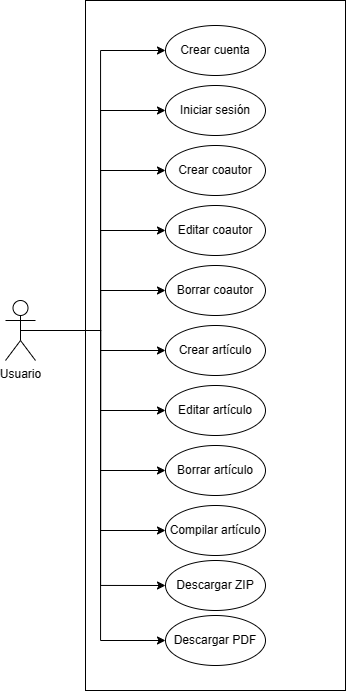
\includegraphics[scale=0.5]{IMAGENES/caso-uso.png}
    \caption{Diagrama de Casos de Uso del Sistema de Gestión de Artículos}
    \label{fig:casos-uso}
\end{figure}

Para un mejor entendimiento de los casos de uso, se decidió hacer el modelado de los requisitos obtenidos para conocer todas las actividades, flujos de información y manejo de errores de cada una de las acciones que hará el usuario.

En el cuadro \ref{tab:caso-uso-crear-cuenta} se muestra el caso de uso para la creación de una cuenta de usuario en el sistema. En este caso, el usuario debe ingresar su nombre, datos de autor, correo electrónico y contraseña para crear una cuenta. Si los datos son válidos, el sistema le permitirá crear la cuenta y acceder a su perfil. En caso de que los datos sean incorrectos o ya exista una cuenta con el mismo correo electrónico, el sistema mostrará un mensaje de error y le dará la opción de intentarlo nuevamente.

\begin{table}[H]
    \centering
        \begin{tabular}{|p{0.5cm}|p{3.5cm}|p{10cm}|}
        \hline
        \textbf{ID} & \textbf{Caso de Uso} & \textbf{Crear Cuenta} \\
        \hline
        1 & \textbf{Descripción} & El usuario crea una cuenta en el sistema. \\
        \hline
        2 & \textbf{Actores} & Usuario. \\
        \hline
        3 & \textbf{Precondiciones} & El usuario no debe tener una cuenta en el sistema. \\
        \hline
        4 & \textbf{Flujo Principal} & 
        \begin{enumerate}
            \item El usuario ingresa su nombre, datos de autor, correo electrónico y contraseña.
            \item El sistema verifica los datos ingresados.
            \item El sistema crea la cuenta del usuario.
        \end{enumerate} \\
        \hline
        5 & \textbf{Flujo Alternativo} & 
        \begin{enumerate}
            \item El sistema muestra un mensaje de error si los datos son incorrectos o ya existe una cuenta con el mismo correo electrónico.
            \item El usuario puede intentarlo nuevamente.
        \end{enumerate} \\
        \hline
        6 & \textbf{Postcondiciones} & El usuario crea una cuenta en el sistema. \\
        \hline
    \end{tabular}
    \caption{Caso de Uso: Crear Cuenta}
    \label{tab:caso-uso-crear-cuenta}
\end{table}

En el cuadro \ref{tab:caso-uso-iniciar-sesion} se muestra el caso de uso para el inicio de sesión de un usuario en el sistema. En este caso, el usuario debe ingresar su correo electrónico y contraseña para acceder al sistema. Si los datos son correctos, el sistema le permitirá acceder a su perfil. En caso de que los datos sean incorrectos, el sistema mostrará un mensaje de error y le dará la opción de intentarlo nuevamente.

\begin{table}[H]
    \centering
        \begin{tabular}{|p{0.5cm}|p{3.5cm}|p{10cm}|}
        \hline
        \textbf{ID} & \textbf{Caso de Uso} & \textbf{Iniciar Sesión} \\
        \hline
        1 & \textbf{Descripción} & El usuario inicia sesión en el sistema. \\
        \hline
        2 & \textbf{Actores} & Usuario. \\
        \hline
        3 & \textbf{Precondiciones} & El usuario debe tener una cuenta en el sistema. \\
        \hline
        4 & \textbf{Flujo Principal} & 
        \begin{enumerate}
            \item El usuario ingresa su correo electrónico y contraseña.
            \item El sistema verifica los datos ingresados.
            \item El sistema muestra el perfil del usuario.
        \end{enumerate} \\
        \hline
        5 & \textbf{Flujo Alternativo} & 
        \begin{enumerate}
            \item El sistema muestra un mensaje de error si los datos son incorrectos.
            \item El usuario puede intentarlo nuevamente.
        \end{enumerate} \\
        \hline
        6 & \textbf{Postcondiciones} & El usuario accede a su perfil en el sistema. \\
        \hline
    \end{tabular}
    \caption{Caso de Uso: Iniciar Sesión}
    \label{tab:caso-uso-iniciar-sesion}
\end{table}

En el cuadro \ref{tab:caso-uso-crear-articulo} se muestra el caso de uso para la creación de un artículo en el sistema. En este caso, el usuario debe ingresar los datos del artículo, como el título, el contenido y las referencias. El sistema le permitirá guardar el artículo y compilarlo en una plantilla LaTeX. Si el artículo se guarda correctamente, el sistema mostrará un mensaje de confirmación y le dará la opción de descargar el PDF generado.

\begin{table}[H]
    \centering
        \begin{tabular}{|p{0.5cm}|p{3.5cm}|p{10cm}|}
        \hline
        \textbf{ID} & \textbf{Caso de Uso} & \textbf{Crear Artículo} \\
        \hline
        1 & \textbf{Descripción} & El usuario crea un artículo en el sistema. \\
        \hline
        2 & \textbf{Actores} & Usuario. \\
        \hline
        3 & \textbf{Precondiciones} & El usuario debe haber iniciado sesión en el sistema. \\
        \hline
        4 & \textbf{Flujo Principal} & 
        \begin{enumerate}
            \item El usuario ingresa el título, contenido y referencias del artículo.
            \item El sistema guarda el artículo.
            \item El sistema compila el artículo en una plantilla LaTeX.
            \item El sistema muestra un mensaje de confirmación.
        \end{enumerate} \\
        \hline
        5 & \textbf{Flujo Alternativo} & 
        \begin{enumerate}
            \item El sistema muestra un mensaje de error si los datos son incorrectos.
            \item El usuario puede intentarlo nuevamente.
        \end{enumerate} \\
        \hline
        6 & \textbf{Postcondiciones} & El usuario crea un artículo en el sistema. \\
        \hline
    \end{tabular}
    \caption{Caso de Uso: Crear Artículo}
    \label{tab:caso-uso-crear-articulo}

\end{table}

En el cuadro \ref{tab:caso-uso-editar-articulo} se muestra el caso de uso para la edición de un artículo en el sistema. En este caso, el usuario puede editar los datos del artículo, como el título, el contenido, los coautores y las referencias. El sistema le permitirá guardar los cambios y compilar el artículo en una plantilla LaTeX. Si los cambios se guardan correctamente, el sistema mostrará un mensaje de confirmación y le dará la opción de descargar el PDF generado.

\begin{table}[H]
    \centering
        \begin{tabular}{|p{0.5cm}|p{3.5cm}|p{10cm}|}
        \hline
        \textbf{ID} & \textbf{Caso de Uso} & \textbf{Editar Artículo} \\
        \hline
        1 & \textbf{Descripción} & El usuario edita un artículo en el sistema. \\
        \hline
        2 & \textbf{Actores} & Usuario. \\
        \hline
        3 & \textbf{Precondiciones} & El usuario debe haber iniciado sesión en el sistema y tener un artículo creado. \\
        \hline
        4 & \textbf{Flujo Principal} & 
        \begin{enumerate}
            \item El usuario selecciona el artículo a editar.
            \item El usuario edita los datos del artículo.
            \item El sistema guarda los cambios.
            \item El sistema compila el artículo en una plantilla LaTeX.
            \item El sistema muestra un mensaje de confirmación.
        \end{enumerate} \\
        \hline
        5 & \textbf{Flujo Alternativo} & 
        \begin{enumerate}
            \item El sistema muestra un mensaje de error si los datos son incorrectos.
            \item El usuario puede intentarlo nuevamente.
        \end{enumerate} \\
        \hline
        6 & \textbf{Postcondiciones} & El usuario edita un artículo en el sistema. \\
        \hline
    \end{tabular}
    \caption{Caso de Uso: Editar Artículo}
    \label{tab:caso-uso-editar-articulo}
\end{table}



En el cuadro \ref{tab:caso-uso-borrar-articulo} se muestra el caso de uso para la eliminación de un artículo en el sistema. En este caso, el usuario puede seleccionar un artículo y borrarlo del sistema. El sistema le mostrará un mensaje de confirmación y le dará la opción de borrar el artículo definitivamente.

\begin{table}[H]
    \centering
        \begin{tabular}{|p{0.5cm}|p{3.5cm}|p{10cm}|}
        \hline
        \textbf{ID} & \textbf{Caso de Uso} & \textbf{Borrar Artículo} \\
        \hline
        1 & \textbf{Descripción} & El usuario borra un artículo en el sistema. \\
        \hline
        2 & \textbf{Actores} & Usuario. \\
        \hline
        3 & \textbf{Precondiciones} & El usuario debe haber iniciado sesión en el sistema y tener un artículo creado. \\
        \hline
        4 & \textbf{Flujo Principal} & 
        \begin{enumerate}
            \item El usuario selecciona el artículo a borrar.
            \item El sistema muestra un mensaje de confirmación.
            \item El usuario confirma la eliminación del artículo.
        \end{enumerate} \\
        \hline
        5 & \textbf{Flujo Alternativo} & 
        \begin{enumerate}
            \item El usuario cancela la eliminación del artículo.
            \item El sistema muestra un mensaje de confirmación.
        \end{enumerate} \\
        \hline
        6 & \textbf{Postcondiciones} & El usuario borra un artículo en el sistema. \\
        \hline
    \end{tabular}
    \caption{Caso de Uso: Borrar Artículo}
    \label{tab:caso-uso-borrar-articulo}
\end{table}

En el cuadro \ref{tab:caso-uso-crear-coautor} se muestra el caso de uso para la creación de un coautor en el sistema. En este caso, el usuario puede agregar un coator a la lista de coautores con los que ha trabajado en un artículo. El sistema le permitirá guardar los cambios y mostrará un mensaje de confirmación si la operación es exitosa.

\begin{table}[H]
    \centering
        \begin{tabular}{|p{0.5cm}|p{3.5cm}|p{10cm}|}
        \hline
        \textbf{ID} & \textbf{Caso de Uso} & \textbf{Crear Coautor} \\
        \hline
        1 & \textbf{Descripción} & El usuario crea un coautor en el sistema. \\
        \hline
        2 & \textbf{Actores} & Usuario. \\
        \hline
        3 & \textbf{Precondiciones} & El usuario debe haber iniciado sesión en el sistema y tener un artículo creado. \\
        \hline
        4 & \textbf{Flujo Principal} & 
        \begin{enumerate}
            \item El usuario selecciona el artículo al que desea agregar un coautor.
            \item El usuario agrega el coautor a la lista de coautores.
            \item El sistema guarda los cambios.
            \item El sistema muestra un mensaje de confirmación.
        \end{enumerate} \\
        \hline
        5 & \textbf{Flujo Alternativo} & 
        \begin{enumerate}
            \item El sistema muestra un mensaje de error si los datos son incorrectos.
            \item El usuario puede intentarlo nuevamente.
        \end{enumerate} \\
        \hline
        6 & \textbf{Postcondiciones} & El usuario crea un coautor en el sistema. \\
        \hline
    \end{tabular}
    \caption{Caso de Uso: Crear Coautor}
    \label{tab:caso-uso-crear-coautor}

\end{table}

En el cuadro \ref{tab:caso-uso-editar-coautor} se muestra el caso de uso para la edición de un coautor en el sistema. En este caso, el usuario puede seleccionar un coautor y editar sus datos. El sistema le permitirá guardar los cambios y mostrará un mensaje de confirmación si la operación es exitosa.

\begin{table}[H]
    \centering
        \begin{tabular}{|p{0.5cm}|p{3.5cm}|p{10cm}|}
        \hline
        \textbf{ID} & \textbf{Caso de Uso} & \textbf{Editar Coautor} \\
        \hline
        1 & \textbf{Descripción} & El usuario edita un coautor en el sistema. \\
        \hline
        2 & \textbf{Actores} & Usuario. \\
        \hline
        3 & \textbf{Precondiciones} & El usuario debe haber iniciado sesión en el sistema y tener un coautor creado. \\
        \hline
        4 & \textbf{Flujo Principal} & 
        \begin{enumerate}
            \item El usuario selecciona el coautor a editar.
            \item El usuario edita los datos del coautor.
            \item El sistema guarda los cambios.
            \item El sistema muestra un mensaje de confirmación.
        \end{enumerate} \\
        \hline
        5 & \textbf{Flujo Alternativo} & 
        \begin{enumerate}
            \item El sistema muestra un mensaje de error si los datos son incorrectos.
            \item El usuario puede intentarlo nuevamente.
        \end{enumerate} \\
        \hline
        6 & \textbf{Postcondiciones} & El usuario edita un coautor en el sistema. \\
        \hline
    \end{tabular}
    \caption{Caso de Uso: Editar Coautor}
    \label{tab:caso-uso-editar-coautor}

\end{table}

En el cuadro \ref{tab:caso-uso-borrar-coautor} se muestra el caso de uso para la eliminación de un coautor en el sistema. En este caso, el usuario puede seleccionar un coautor y borrarlo del sistema. El sistema le mostrará un mensaje de confirmación y le dará la opción de borrar el coautor definitivamente.

\begin{table}[H]
    \centering
        \begin{tabular}{|p{0.5cm}|p{3.5cm}|p{10cm}|}
        \hline
        \textbf{ID} & \textbf{Caso de Uso} & \textbf{Borrar Coautor} \\
        \hline
        1 & \textbf{Descripción} & El usuario borra un coautor en el sistema. \\
        \hline
        2 & \textbf{Actores} & Usuario. \\
        \hline
        3 & \textbf{Precondiciones} & El usuario debe haber iniciado sesión en el sistema y tener un coautor creado. \\
        \hline
        4 & \textbf{Flujo Principal} & 
        \begin{enumerate}
            \item El usuario selecciona el coautor a borrar.
            \item El sistema muestra un mensaje de confirmación.
            \item El usuario confirma la eliminación del coautor.
        \end{enumerate} \\
        \hline
        5 & \textbf{Flujo Alternativo} & 
        \begin{enumerate}
            \item El usuario cancela la eliminación del coautor.
            \item El sistema muestra un mensaje de confirmación.
        \end{enumerate} \\
        \hline
        6 & \textbf{Postcondiciones} & El usuario borra un coautor en el sistema. \\
        \hline
    \end{tabular}
    \caption{Caso de Uso: Borrar Coautor}
    \label{tab:caso-uso-borrar-coautor}
\end{table}

En el cuadro \ref{tab:caso-uso-subir-plantilla} se muestra el caso de uso para la subida de una plantilla LaTeX en formato .zip al sistema. En este caso, el usuario debe seleccionar un archivo .zip que contenga la plantilla LaTeX y subirlo al sistema. El sistema le permitirá guardar la plantilla y mostrará un mensaje de confirmación si la subida es exitosa.

\begin{table}[H]
    \centering
        \begin{tabular}{|p{0.5cm}|p{3.5cm}|p{10cm}|}
        \hline
        \textbf{ID} & \textbf{Caso de Uso} & \textbf{Subir Plantilla LaTeX} \\
        \hline
        1 & \textbf{Descripción} & El usuario sube una plantilla LaTeX al sistema. \\
        \hline
        2 & \textbf{Actores} & Usuario. \\
        \hline
        3 & \textbf{Precondiciones} & El usuario debe haber iniciado sesión en el sistema. \\
        \hline
        4 & \textbf{Flujo Principal} & 
        \begin{enumerate}
            \item El usuario selecciona un archivo .zip que contenga la plantilla LaTeX.
            \item El sistema guarda la plantilla en la base de datos.
            \item El sistema muestra un mensaje de confirmación.
        \end{enumerate} \\
        \hline
        5 & \textbf{Flujo Alternativo} & 
        \begin{enumerate}
            \item El sistema muestra un mensaje de error si el archivo no es válido.
            \item El usuario puede intentarlo nuevamente.
        \end{enumerate} \\
        \hline
        6 & \textbf{Postcondiciones} & El usuario sube una plantilla LaTeX al sistema. \\
        \hline
    \end{tabular}
    \caption{Caso de Uso: Subir Plantilla LaTeX}
\label{tab:caso-uso-subir-plantilla}
\end{table}

En el cuadro \ref{tab:caso-uso-compilar-articulo} se muestra el caso de uso para la compilación de un artículo en una plantilla LaTeX. En este caso, el usuario debe seleccionar un artículo y una plantilla LaTeX para compilar el contenido del artículo en la plantilla. El sistema le permitirá descargar el PDF generado y el archivo ZIP del artículo compilado. 

\begin{table}[H]
    \centering
    \begin{tabular}{|p{0.5cm}|p{3.5cm}|p{10cm}|}
        \hline
        \textbf{ID} & \textbf{Caso de Uso} & \textbf{Compilar Artículo} \\
        \hline
        1 & \textbf{Descripción} & El usuario compila un artículo en una plantilla LaTeX. \\
        \hline
        2 & \textbf{Actores} & Usuario. \\
        \hline
        3 & \textbf{Precondiciones} & El usuario debe haber iniciado sesión en el sistema y tener un artículo creado. \\
        \hline
        4 & \textbf{Flujo Principal} & 
        \begin{enumerate}
            \item El usuario selecciona el artículo a compilar.
            \item El usuario selecciona la plantilla LaTeX en la que compilar el artículo.
            \item El sistema compila el contenido del artículo en la plantilla.
            \item El sistema muestra un mensaje de confirmación.
        \end{enumerate} \\
        \hline
        5 & \textbf{Flujo Alternativo} & 
        \begin{enumerate}
            \item El sistema muestra un mensaje de error si los datos son incorrectos.
            \item El usuario puede intentarlo nuevamente.
        \end{enumerate} \\
        \hline
        6 & \textbf{Postcondiciones} & El usuario compila un artículo en una plantilla LaTeX. \\
        \hline
    \end{tabular}
    \caption{Caso de Uso: Compilar Artículo}
\label{tab:caso-uso-compilar-articulo}

\end{table}

En el cuadro \ref{tab:caso-uso-descargar-pdf} se muestra el caso de uso para la descarga de un PDF generado a partir de un artículo compilado. En este caso, el usuario debe seleccionar un artículo y descargar el PDF generado por el sistema. El sistema le permitirá descargar el PDF y mostrará un mensaje de confirmación si la descarga es exitosa.

\begin{table}[H]
    \centering
    \begin{tabular}{|p{0.5cm}|p{3.5cm}|p{10cm}|}
        \hline
        \textbf{ID} & \textbf{Caso de Uso} & \textbf{Descargar PDF} \\
        \hline
        1 & \textbf{Descripción} & El usuario descarga un PDF generado a partir de un artículo compilado. \\
        \hline
        2 & \textbf{Actores} & Usuario. \\
        \hline
        3 & \textbf{Precondiciones} & El usuario debe haber iniciado sesión en el sistema y tener un artículo compilado. \\
        \hline
        4 & \textbf{Flujo Principal} & 
        \begin{enumerate}
            \item El usuario selecciona el artículo a descargar.
            \item El sistema genera el PDF del artículo.
            \item El sistema permite la descarga del PDF.
        \end{enumerate} \\
        \hline
        5 & \textbf{Flujo Alternativo} & 
        \begin{enumerate}
            \item El sistema muestra un mensaje de error si la descarga falla.
            \item El usuario puede intentarlo nuevamente.
        \end{enumerate} \\
        \hline
        6 & \textbf{Postcondiciones} & El usuario descarga un PDF generado del artículo. \\
        \hline
    \end{tabular}
    \caption{Caso de Uso: Descargar PDF}
    \label{tab:caso-uso-descargar-pdf}

\end{table}

En el cuadro \ref{tab:caso-uso-descargar-zip} se muestra el caso de uso para la descarga de un archivo ZIP generado a partir de un artículo compilado. En este caso, el usuario podrá descargar el archivo ZIP que contiene el PDF generado y los archivos auxiliares del artículo compilado. El sistema le permitirá descargar el archivo ZIP si este se genera correctamente.

\begin{table}[H]
    \centering
    \begin{tabular}{|p{0.5cm}|p{3.5cm}|p{10cm}|}
        \hline
        \textbf{ID} & \textbf{Caso de Uso} & \textbf{Descargar ZIP} \\
        \hline
        1 & \textbf{Descripción} & El usuario descarga un archivo ZIP generado a partir de un artículo compilado. \\
        \hline
        2 & \textbf{Actores} & Usuario. \\
        \hline
        3 & \textbf{Precondiciones} & El usuario debe haber iniciado sesión en el sistema y tener un artículo compilado. \\
        \hline
        4 & \textbf{Flujo Principal} & 
        \begin{enumerate}
            \item El usuario selecciona el artículo a descargar.
            \item El sistema genera el archivo ZIP del artículo.
            \item El sistema permite la descarga del archivo ZIP.
        \end{enumerate} \\
        \hline
        5 & \textbf{Flujo Alternativo} & 
        \begin{enumerate}
            \item El sistema muestra un mensaje de error si la descarga falla.
            \item El usuario puede intentarlo nuevamente.
        \end{enumerate} \\
        \hline
        6 & \textbf{Postcondiciones} & El usuario descarga un archivo ZIP generado del artículo. \\
        \hline
    \end{tabular}
    \caption{Caso de Uso: Descargar ZIP}
\label{tab:caso-uso-descargar-zip}

\end{table}

\subsection{Diseño de la Base de Datos}
El diseño de la base de datos fue un aspecto fundamental en el desarrollo del sistema de gestión de artículos. Se utilizó MySQL como gestor de base de datos y se implementó un modelo relacional para almacenar la información de los usuarios, plantillas y artículos del sistema. Cabe resaltar que la base de datos se creó utilizando migraciones de Laravel, lo que facilita la creación y modificación de la estructura de la base de datos de manera programática a través de código PHP. No fue necesario escribir consultas SQL directamente, ya que Laravel proporciona una interfaz orientada a objetos para interactuar con la base de datos.

La base de datos del sistema consta de las siguientes tablas:

\begin{itemize}
    \item \textbf{users}: Almacena la información de los usuarios del sistema, como el nombre, apellidos, correo electrónico, contraseña, teléfono, país, dirección, institución, dirección de la institución, biografía, ORCID, afiliación, foto de perfil y fecha de creación.
    \item \textbf{articles}: Almacena la información de los artículos creados por los usuarios, como el título, resumen, contenido, palabras clave, referencias, usuario creador y fechas de creación y actualización.
    \item \textbf{coauthors}: Almacena la información de los coautores de los artículos, como el nombre, apellidos, correo electrónico, teléfono, país, dirección, institución, dirección de la institución, afiliación, ORCID, URL de la afiliación, usuario creador y fechas de creación y actualización.
    \item \textbf{coauthor\_article}: Almacena la relación entre los coautores y los artículos, con las claves foráneas de los coautores y los artículos.
    \item \textbf{templates}: Almacena la información de las plantillas LaTeX subidas por los usuarios, como el nombre, descripción, archivo, usuario creador y fechas de creación y actualización.
\end{itemize}

Se pensó en un diseño de base de datos relacional para almacenar la información de los usuarios, plantillas y artículos del sistema, esto con el fin de tener una estructura de datos que permita relacionar la información de los usuarios con los artículos y las plantillas, y así poder realizar consultas y operaciones de manera eficiente, utilizando las relaciones entre las tablas. Además, se implementaron restricciones de clave foránea para mantener la integridad referencial de la base de datos y asegurar que los datos estén correctamente relacionados entre sí.

\subsubsection{Diagrama Entidad-Relación}
En el desarrollo del sistema, también se diseó el diagrama entidad-relación de la base de datos, con las entidades y relaciones entre ellas. La figura \ref{fig:diagrama-er} muestra el diagrama entidad-relación de la base de datos del sistema de gestión de artículos, con las entidades y relaciones entre ellas. Se puede observar que las entidades \textit{users}, \textit{articles}, \textit{coauthors} y \textit{templates} están relacionadas entre sí a través de las relaciones \textit{coauthor\_article} y \textit{articles\_user}. La relación \textit{coauthor\_article} permite relacionar los coautores con los artículos, mientras que la relación \textit{articles\_user} permite relacionar los artículos con los usuarios que los crearon.

\begin{figure}[H]
    \centering
    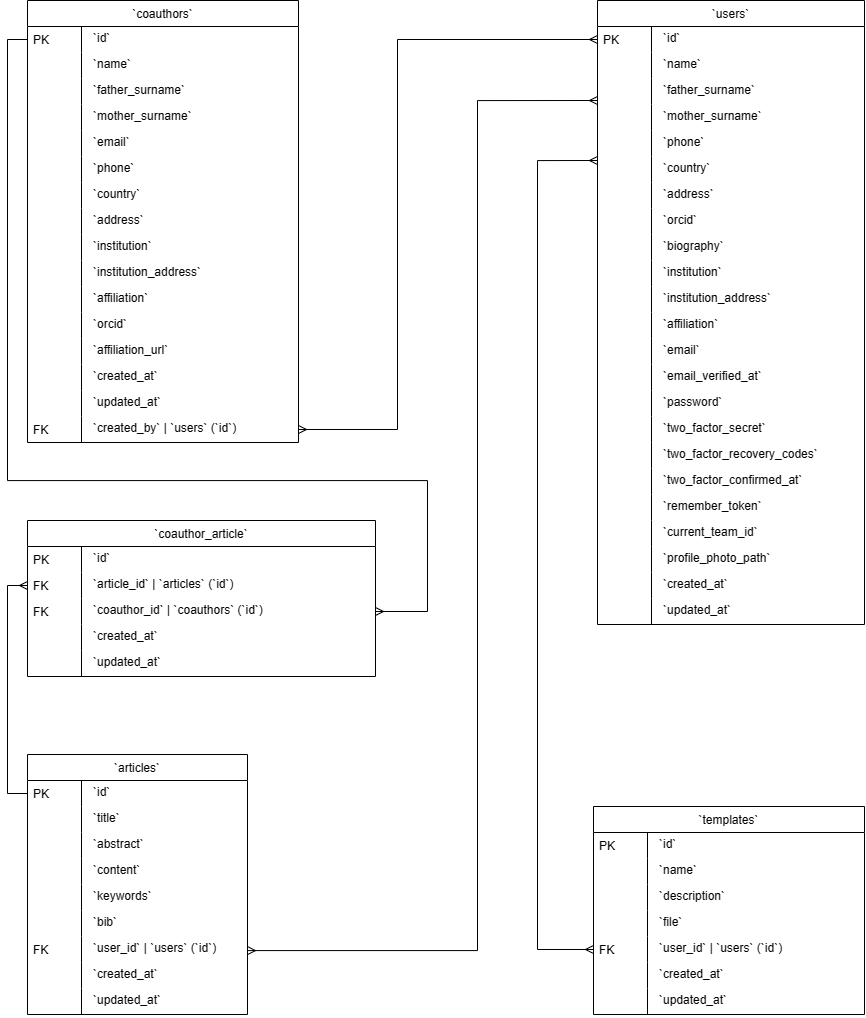
\includegraphics[width=1\textwidth]{IMAGENES/entidad-relacion.png}
    \caption{Diagrama Entidad-Relación de la Base de Datos}
\label{fig:diagrama-er}
\end{figure}

\subsection{Diccionario de Datos}
Para conocer a detalle la composición de las tablas que integran la base de datos, se desarrolló un diccionario de datos conformado por las tablas \ref{tab:users}, \ref{tab:articles}, \ref{tab:coauthors}, \ref{tab:coauthor_article}, \ref{tab:templates} donde se describe de manera específica todos los campos y tipo de dato contenidos en cada una de las tablas, a fin de entender su función.

\begin{table}[H]
    \centering
    \begin{tabular}{|p{5cm}|p{3cm}|p{1cm}|p{2cm}|p{2cm}|}
        \hline
        \textbf{Campo} & \textbf{Tipo de Dato} & \textbf{Nulo} & \textbf{Llave Primaria} & \textbf{Llave Foránea} \\
        \hline
        id & bigint UNSIGNED & No & Sí & No \\
        name & varchar(255) & No & No & No \\
        father\_surname & varchar(255) & No & No & No \\
        mother\_surname & varchar(255) & No & No & No \\
        phone & varchar(255) & No & No & No \\
        country & varchar(255) & No & No & No \\
        address & varchar(255) & Sí & No & No \\
        orcid & varchar(255) & Sí & No & No \\
        biography & text & Sí & No & No \\
        institution & varchar(255) & No & No & No \\
        institution\_address & varchar(255) & No & No & No \\
        affiliation & varchar(255) & Sí & No & No \\
        email & varchar(255) & No & No & No \\
        password & varchar(255) & No & No & No \\
        profile\_photo\_path & varchar(2048) & Sí & No & No \\
        created\_at & timestamp & Sí & No & No \\
        updated\_at & timestamp & Sí & No & No \\
        \hline
    \end{tabular}
    \caption{Tabla: users}
    \label{tab:users}
\end{table}

\begin{table}[H]
    \centering
    \begin{tabular}{|p{5cm}|p{3cm}|p{1cm}|p{2cm}|p{2cm}|}
        \hline
        \textbf{Campo} & \textbf{Tipo de Dato} & \textbf{Nulo} & \textbf{Llave Primaria} & \textbf{Llave Foránea} \\
        \hline
        id & bigint UNSIGNED & No & Sí & No \\
        title & varchar(255) & No & No & No \\
        abstract & text & Sí & No & No \\
        content & text & No & No & No \\
        keywords & text & Sí & No & No \\
        bib & text & Sí & No & No \\
        user\_id & bigint UNSIGNED & No & No & Sí \\
        created\_at & timestamp & Sí & No & No \\
        updated\_at & timestamp & Sí & No & No \\
        \hline
    \end{tabular}
    \caption{Tabla: articles}
    \label{tab:articles}

\end{table}

\begin{table}[H]
    \centering
    \begin{tabular}{|p{5cm}|p{3cm}|p{1cm}|p{2cm}|p{2cm}|}
        \hline
        \textbf{Campo} & \textbf{Tipo de Dato} & \textbf{Nulo} & \textbf{Llave Primaria} & \textbf{Llave Foránea} \\
        \hline
        id & bigint UNSIGNED & No & Sí & No \\
        name & varchar(255) & No & No & No \\
        father\_surname & varchar(255) & No & No & No \\
        mother\_surname & varchar(255) & No & No & No \\
        email & varchar(255) & No & No & No \\
        phone & varchar(255) & No & No & No \\
        country & varchar(255) & No & No & No \\
        address & varchar(255) & No & No & No \\
        institution & varchar(255) & No & No & No \\
        institution\_address & varchar(255) & No & No & No \\
        affiliation & varchar(255) & Sí & No & No \\
        orcid & varchar(255) & No & No & No \\
        affiliation\_url & varchar(255) & Sí & No & No \\
        created\_at & timestamp & Sí & No & No \\
        updated\_at & timestamp & Sí & No & No \\
        created\_by & bigint UNSIGNED & No & No & Sí \\
        \hline
    \end{tabular}
    \caption{Tabla: coauthors}
    \label{tab:coauthors}

\end{table}

\begin{table}[H]
    \centering
    \begin{tabular}{|p{5cm}|p{3cm}|p{1cm}|p{2cm}|p{2cm}|}
        \hline
        \textbf{Campo} & \textbf{Tipo de Dato} & \textbf{Nulo} & \textbf{Llave Primaria} & \textbf{Llave Foránea} \\
        \hline
        id & bigint UNSIGNED & No & Sí & No \\
        article\_id & bigint UNSIGNED & No & No & Sí \\
        coauthor\_id & bigint UNSIGNED & No & No & Sí \\
        created\_at & timestamp & Sí & No & No \\
        updated\_at & timestamp & Sí & No & No \\
        \hline
    \end{tabular}
    \caption{Tabla: coauthor\_article}
    \label{tab:coauthor_article}

\end{table}

\begin{table}[H]
    \centering
    \begin{tabular}{|p{5cm}|p{3cm}|p{1cm}|p{2cm}|p{2cm}|}
        \hline
        \textbf{Campo} & \textbf{Tipo de Dato} & \textbf{Nulo} & \textbf{Llave Primaria} & \textbf{Llave Foránea} \\
        \hline
        id & bigint UNSIGNED & No & Sí & No \\
        name & varchar(255) & No & No & No \\
        description & text & Sí & No & No \\
        file & varchar(255) & No & No & No \\
        user\_id & bigint UNSIGNED & No & No & Sí \\
        created\_at & timestamp & Sí & No & No \\
        updated\_at & timestamp & Sí & No & No \\
        \hline
    \end{tabular}
    \caption{Tabla: templates}
    \label{tab:templates}

\end{table}

\subsection{Diseño de la Interfaz de Usuario}
El diseño de la interfaz de usuario fue un aspecto importante en el desarrollo de este sistema ya que se necesitaba una interfaz amigable y responsiva que permitiera a los usuarios interactuar con el sistema de manera sencilla y eficiente. Los diseños de la interfaz de usuario se realizaron desde un inicio usando la herramienta Figma, que permite crear prototipos de alta fidelidad y realizar pruebas de usabilidad antes de empezar con el desarrollo del sistema.

Se diseñaron las interfaces de usuario para las diferentes funcionalidades del sistema, como la creación de artículos, la gestión de coautores, la subida de plantillas LaTeX, entre otras. Se crearon prototipos de alta fidelidad para algunas de las pantallas del sistema, con el objetivo de tener una guía visual para el desarrollo de la interfaz de usuario y también tener retroalimentación de los usuarios sobre el diseño de la interfaz y el flujo de interacción del sistema.

\subsubsection{Prototipos de Alta Fidelidad}
En la figura \ref{fig:prototipo-dashboard} se muestra el prototipo de alta fidelidad de la pantalla de inicio del sistema, donde los usuarios pueden ver una lista de los artículos creados y a un costado un menú de navegación con las diferentes opciones del sistema. En esta pantalla se muestra una tabla con los artículos creados por el usuario, con la opción de ver, editar y borrar cada artículo.

\begin{figure}[H]
    \centering
    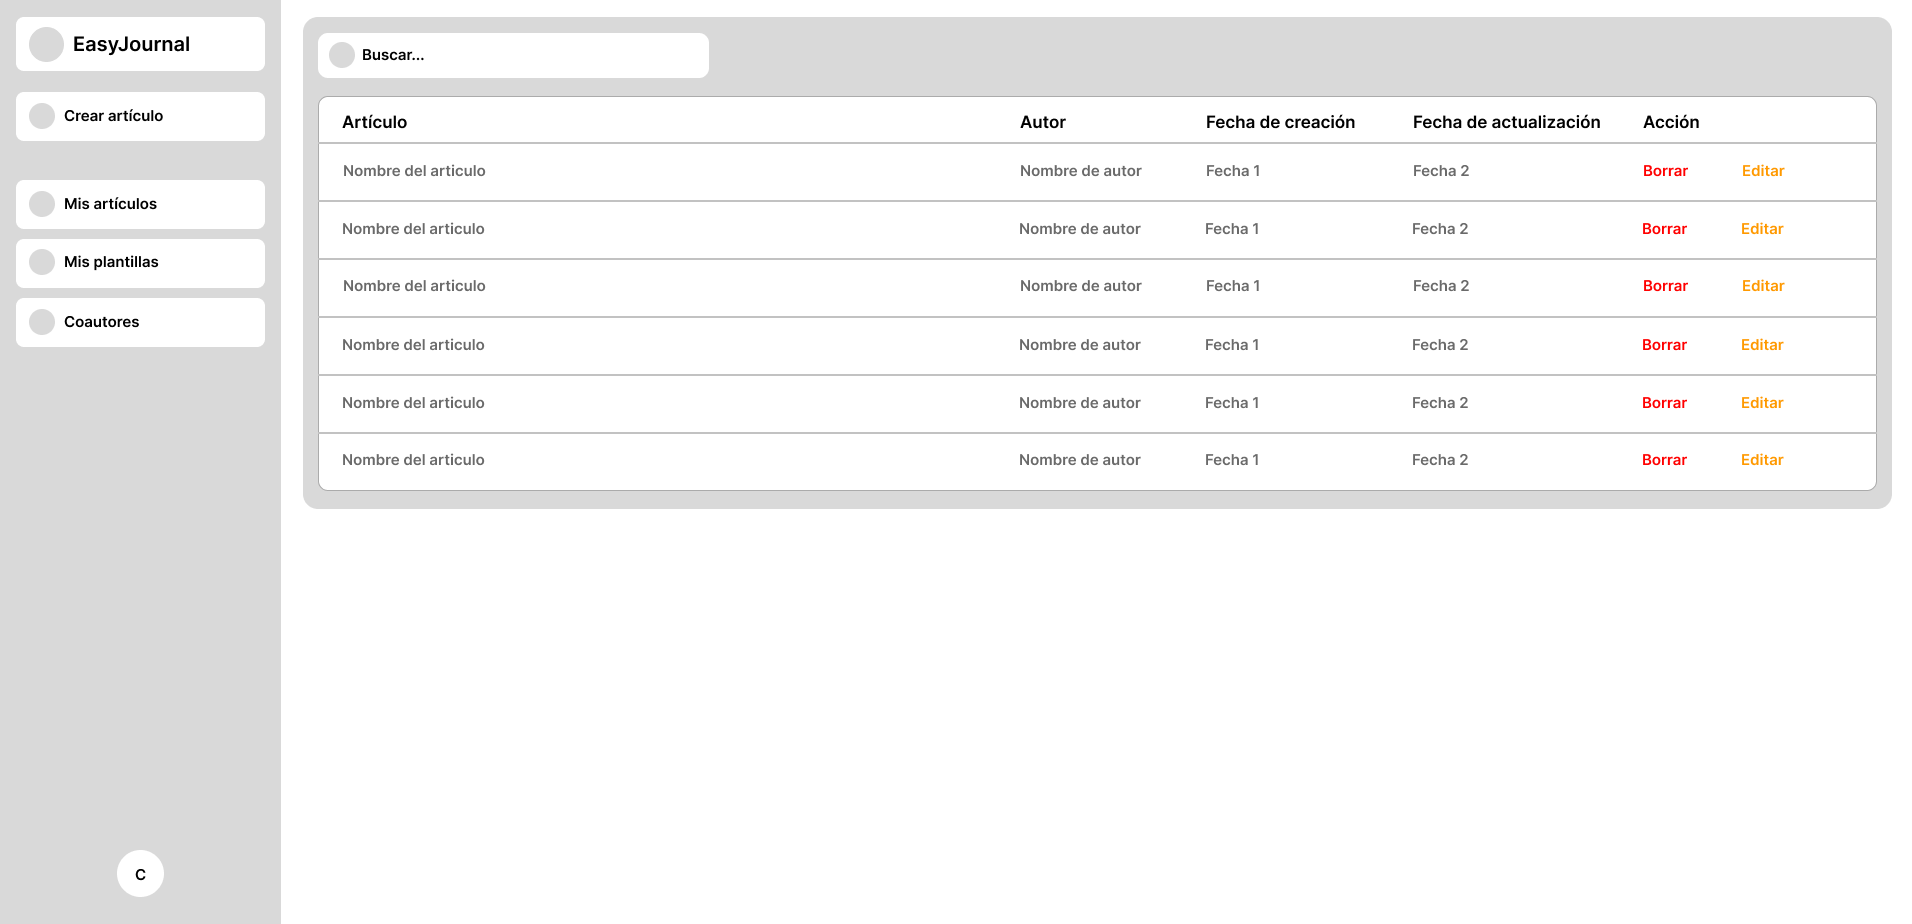
\includegraphics[width=1\textwidth]{IMAGENES/prototipo-dashboard.png}
    \caption{Prototipo de Alta Fidelidad: Pantalla de Inicio del Sistema}
\label{fig:prototipo-dashboard}

\end{figure}

En la figura \ref{fig:prototipo-crear-articulo} se muestra el prototipo de alta fidelidad de la pantalla de creación de un artículo en el sistema, donde los usuarios pueden ingresar el título del artículo y crearlo. En esta pantalla se muestra un formulario con el campo de título y un botón para guardar el artículo en el sistema.

\begin{figure}[H]
    \centering
    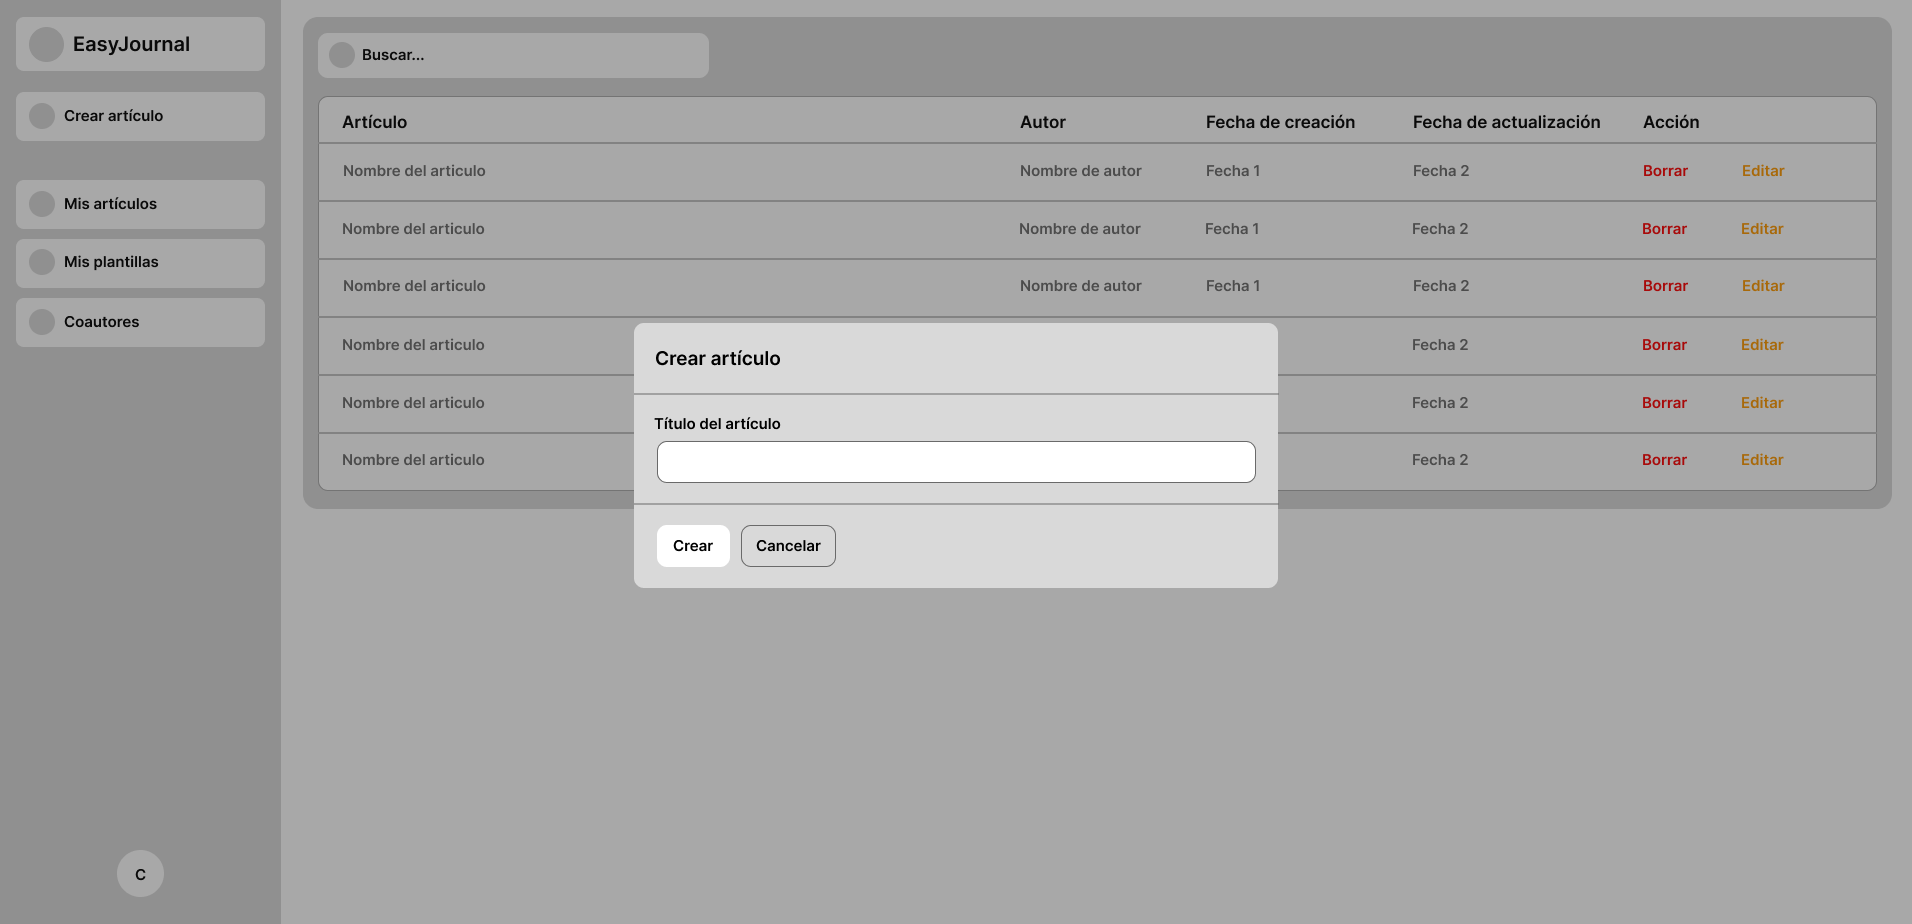
\includegraphics[width=1\textwidth]{IMAGENES/prototipo-crear-articulo.png}
    \caption{Prototipo de Alta Fidelidad: Pantalla de Creación de Artículo}
\label{fig:prototipo-crear-articulo}

\end{figure}

% En la figura \ref{fig:prototipo-crear-coautor} se muestra el prototipo de alta fidelidad de la pantalla de creación de un coautor en el sistema, donde los usuarios pueden ingresar los datos del coautor y guardarlo. En esta pantalla se muestran los campos de nombre, apellidos, correo electrónico, teléfono, país, dirección, institución, dirección de la institución, afiliación, ORCID y URL de la afiliación del coautor, y a un costado se ve una lista de los coautores creados.

% \begin{figure}[H]
%     \centering
%     \includegraphics[width=1\textwidth]{IMAGENES/prototipo-crear-coautor.png}
%     \caption{Prototipo de Alta Fidelidad: Pantalla de Creación de Coautor}
% \label{fig:prototipo-crear-coautor}

% \end{figure}


En la figura \ref{fig:prototipo-subir-plantilla} se muestra el prototipo de alta fidelidad de la pantalla de subida de una plantilla LaTeX en el sistema, donde los usuarios pueden seleccionar un archivo .zip que contenga la plantilla y subirla al sistema. En esta pantalla se muestra un formulario con el campo de archivo, nombre, descripción y un botón para subir la plantilla al sistema.

\begin{figure}[H]
    \centering
    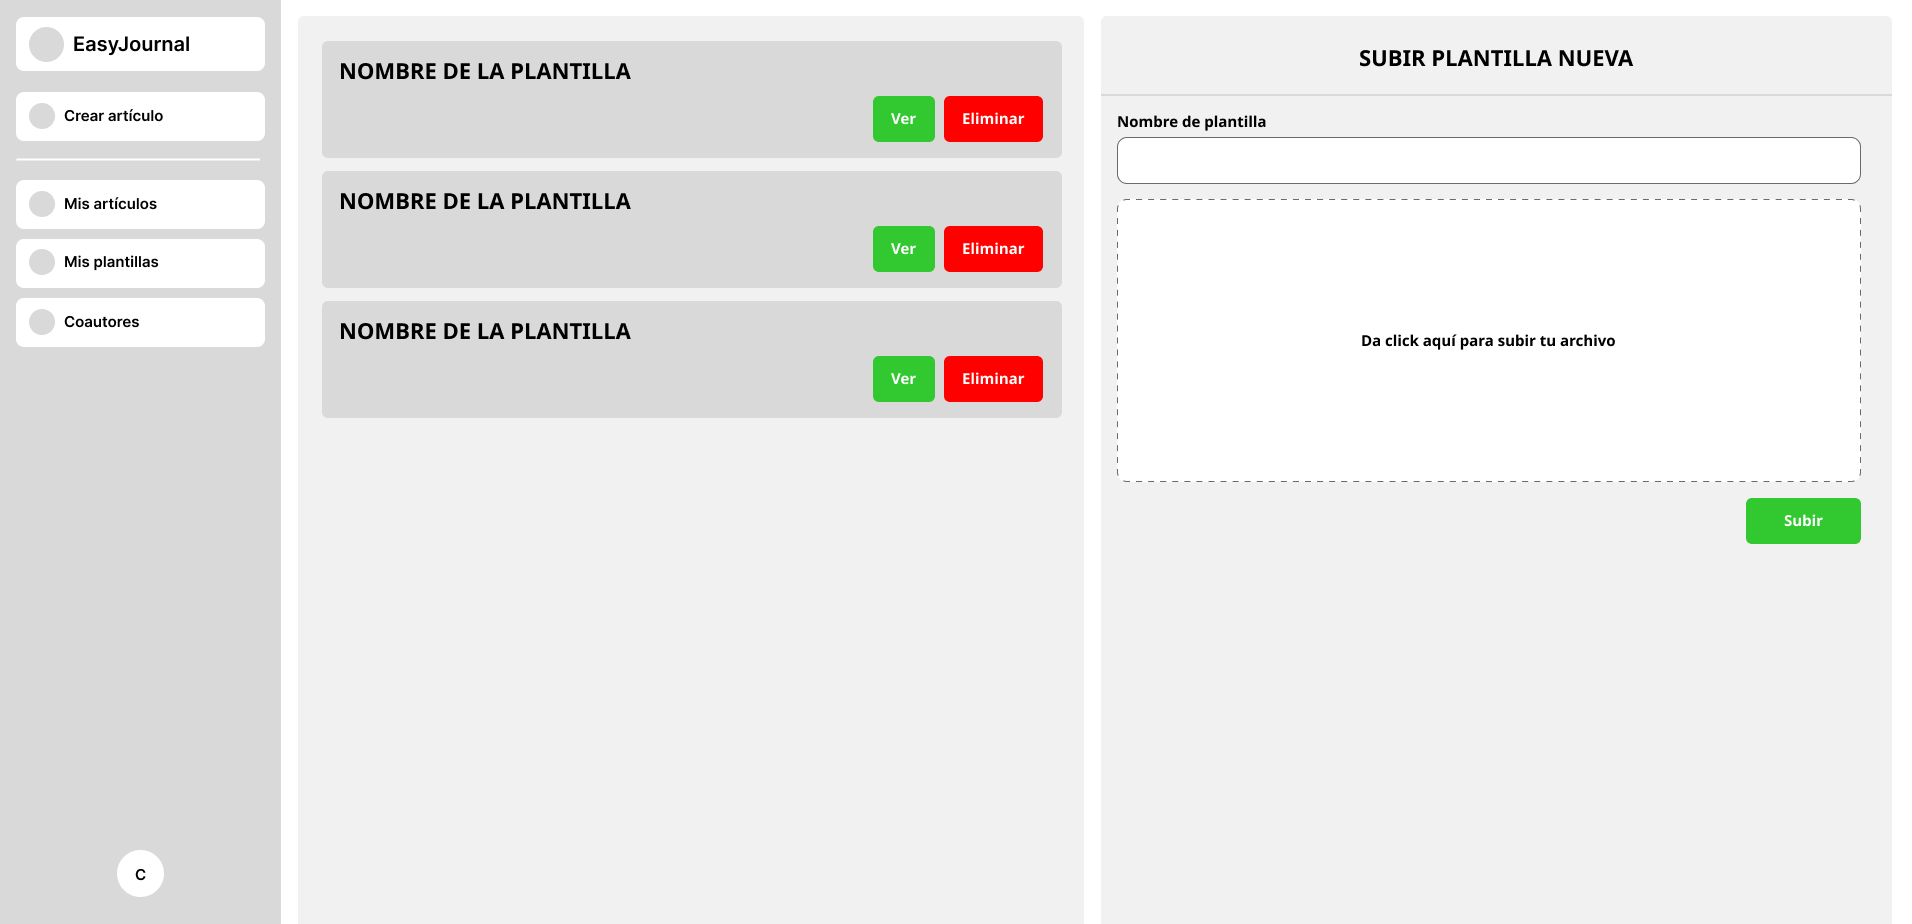
\includegraphics[width=1\textwidth]{IMAGENES/prototipo-subir-plantilla.png}
    \caption{Prototipo de Alta Fidelidad: Pantalla de Subida de Plantilla LaTeX}
\label{fig:prototipo-subir-plantilla}

\end{figure}

En la figura \ref{fig:prototipo-compilar-articulo} se muestra el prototipo de alta fidelidad de la pantalla de compilación de un artículo en una plantilla LaTeX, donde los usuarios pueden seleccionar un artículo y una plantilla para compilar el contenido del artículo en la plantilla. En esta pantalla se muestran los campos de artículo y plantilla, con la opción de compilar el artículo en la plantilla y descargar el PDF generado.

\begin{figure}[H]
    \centering
    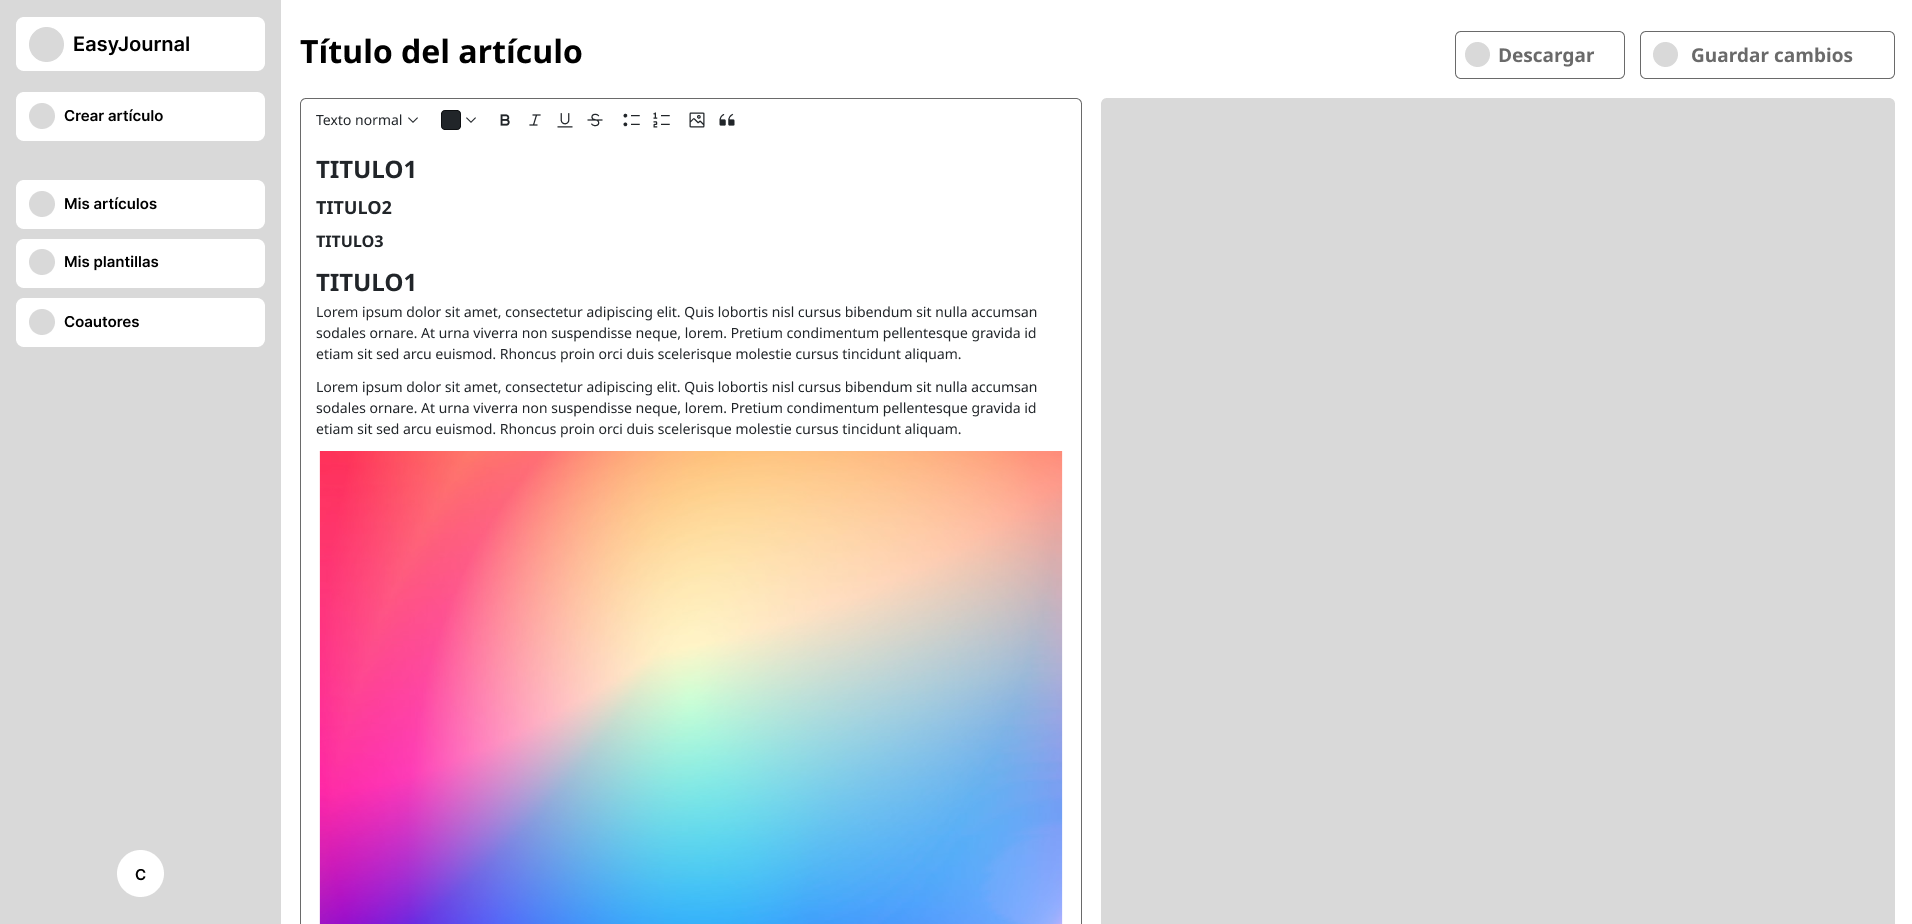
\includegraphics[width=1\textwidth]{IMAGENES/prototipo-compilar-articulo.png}
    \caption{Prototipo de Alta Fidelidad: Pantalla de Compilación de Artículo}
\label{fig:prototipo-compilar-articulo}

\end{figure}

\subsection{Desarrollo del Backend}
El desarrollo del backend del sistema se realizó utilizando el framework de php Laravel, primero se hizo la base instalando Laravel 10, luego se instaló Jetstream para manejar las sesiones, registros, recuperación de contraseñas, entre otras funcionalidades. Después de eso, se instalaron herramientas como Flowbite con Tailwind CSS, EditorJS, Symfony Process, y Gemini, se crearon migraciones, se agregaron rutas y controladores, se implementaron las funcionalidades CRUD (Crear, Leer, Actualizar, Eliminar) y se realizaron pruebas para garantizar el correcto funcionamiento del sistema. A continuación, se describe detalladamente el proceso de desarrollo del backend, incluyendo la instalación de las herramientas necesarias y la implementación de diversas funcionalidades críticas para el sistema.

\subsubsection{Instalación del Entorno de Desarrollo}
El primer paso para el desarrollo del backend fue configurar el entorno de desarrollo adecuado. Se eligió el sistema operativo Linux Mint 20.2 debido a su estabilidad y compatibilidad con las herramientas necesarias.

El proyecto comenzó con la instalación de PHP 8.2 y Composer, ya que son esenciales para el desarrollo de aplicaciones con Laravel. Una vez instaladas estas herramientas, se procedió a la instalación de Laravel 10, la última versión del framework. Posteriormente, se configuró el archivo de entorno `.env' con la información de la base de datos, datos de conexión al correo electrónico, nombre de la aplicación, llave de cifrado, entre otros parámetros importantes para el funcionamiento correcto de la aplicación.

Además, se instaló pdflatex-full junto con sus fuentes para evitar problemas al compilar plantillas que utilizan estas extensiones de LaTeX. Esta instalación fue crucial para asegurar que todos los documentos LaTeX se pudieran compilar correctamente, sin errores relacionados con fuentes o paquetes faltantes.


\subsubsection{Configuración de Jetstream}
Una vez instalado y configurado Laravel, el siguiente paso fue añadir Jetstream para gestionar la autenticación y otras funcionalidades relacionadas con los usuarios. Este paso fue de suma importancia realizarlo al inicio del proyecto antes de agregar otras funcionalidades a la aplicación, ya que Jetstream proporciona una base de archivos y rutas que facilitan la creación de un sistema de autenticación. Configurar Jetstream desde el principio evita problemas futuros al agregar funcionalidades adicionales relacionadas con los usuarios y migraciones de la base de datos.

Una vez instalado Jetstream, se configuraron las funcionalidades de usuario necesarias para el sistema desde el archivo de rutas `web.php', esto para determinar las rutas de redirección para acciones de usuario como registro e inicio de sesión, aqui se incluye un paso importante y es crear un grupo de rutas protegidas por autenticación, esto para asegurar que solo los usuarios autenticados puedan acceder a ciertas rutas. Además, se personalizaron las vistas de autenticación, incluyendo formularios de inicio de sesión y registro. Los mensajes de error y éxito mostrados al usuario tras realizar acciones también fueron ajustados.

Adicionalmente, se modificaron las migraciones de los usuarios para incluir campos adicionales relacionados con los datos de autor, como nombre, apellidos, teléfono, país, dirección, institución, dirección de la institución, biografía, ORCID, afiliación y foto de perfil. Estos campos adicionales son necesarios desde el inicio para evitar problemas al agregar funcionalidades relacionadas con los datos de autor en la aplicación. Configurar estos campos desde el principio asegura que la base de datos esté preparada para manejar toda la información requerida por el sistema sin necesidad de realizar modificaciones estructurales significativas en una etapa posterior del desarrollo.

El proceso de integración de Jetstream fue importante en el desarrollo del backend desde este momento para establecer una base sólida de gestión de usuarios, permitiendo funcionalidades avanzadas. Esta integración facilita el desarrollo de la app en gran medida ya que evita la necesidad de crear un sistema de autenticación desde cero, y permite enfocarse en la implementación de otras características del sistema.

\subsubsection{Integración de Tailwind CSS y Flowbite}
Para el diseño de la interfaz de usuario se utilizó Tailwind CSS junto con Flowbite. Esta combinación facilitó la creación de componentes reutilizables. Inicialmente, se instalaron estas dependencias mediante npm y se configuraron los archivos necesarios para incluir Tailwind CSS y Flowbite en el proyecto.

Se crearon componentes reutilizables como botones, formularios, tarjetas e inputs, utilizando las clases de Tailwind CSS, lo que resultó en un patrón de diseño personalizable y responsivo. Adicionalmente, los componentes de Flowbite como modales, tabs y dropdowns facilitaron la incorporación de elementos interactivos y dinámicos en la interfaz de usuario. Esta integración aceleró el proceso de desarrollo al proporcionar componentes listos para usar en cualquier parte de la aplicación, mejorando la coherencia, la usabilidad de la interfaz de usuario y la eficiencia con la cual se crearon las vistas.

\subsubsection{Implementación de EditorJS y Symfony Process}
Para la creación y edición de artículos científicos en formato LaTeX, se integró EditorJS ya que ofrece una interfaz intuitiva y flexible que permite a los usuarios agregar y organizar diferentes tipos de contenido, como texto, imágenes y código LaTeX embebido, de manera sencilla y eficiente.

Además, se utilizó el paquete Symfony Process para ejecutar comandos del sistema desde el código PHP, lo que facilitó la compilación de documentos LaTeX directamente desde la aplicación. El uso de Symfony Process permitío ejecutar comandos que compilan documentos LaTeX, esto da como resultado la generación de archivos PDF a partir de la plantilla que genera el sistema basado en lo que el usuario ha escrito en el editor de texto. Esto permitió a los usuarios generar documentos sin necesidad de abandonar la plataforma. 

\subsubsection{Integración de Gemini para la Gestión de Autores}
Para la edición precisa de autores en la plantilla LaTeX se usó Gemini, esta herramienta permitió mandar la seccion de autores de cualquier plantilla LaTeX junto con los datos del autor y coautores para que la API de Gemini sustituya los datos del autor en la plantilla LaTeX. La API regresa la sección con los datos ya sustituidos y listos para ser compilados.

\subsubsection{Control de Versiones con Git}
Durante el desarrollo se utilizó Github para el control de versiones del código fuente. Se crearon ramas para cada funcionalidad o tarea, lo que permitió trabajar en paralelo en diferentes partes del sistema sin interferir con el trabajo pendiente. Se realizaron commits regulares para mantener un historial de cambios. Esta práctica de control de versiones facilitó la modificación y corrección de errores en el código, y permitió trabajar de manera más eficiente en diferentes aspectos del sistema.

\subsection{Algoritmos}
A continuación se describen los algoritmos implementados en el sistema, los cuales son fundamentales para el correcto funcionamiento de la aplicación y la subida y generación de archivos LaTeX.

\subsubsection{Algoritmo de Subida de Plantilla LaTeX}
El algoritmo \ref{alg:subida-plantilla} de subida de plantilla LaTeX permite a los usuarios subir archivos .zip que contienen plantillas LaTeX a la aplicación. El algoritmo extrae los archivos del .zip, busca los archivos .tex, .cls, .bib, .bst y .sty, y los renombra para evitar conflictos de nombres. Luego, compila el archivo .tex principal y genera un archivo PDF. Finalmente, guarda la plantilla en la base de datos y muestra un mensaje de éxito o error al usuario. El algoritmo se muestra a continuación:

\begin{algorithm}
    \caption{Guardar Plantilla}
    \begin{algorithmic}[1]
    \Procedure{guardar\_plantilla}{solicitud}
        \State Validar campos requeridos en la solicitud
        \If{la validación falla}
            \State Redirigir a la página de plantillas con un mensaje de error
        \Else
            \State Guardar el archivo ZIP en la carpeta de archivos
            \State Extraer los archivos del ZIP
            \If{la extracción es exitosa}
                \State Buscar archivos .tex en la carpeta extraída
                \If{no se encuentran archivos .tex}
                    \State Redirigir a la página de plantillas con un mensaje de error
                \Else
                    \State Identificar el archivo .tex más grande
                    \State Renombrar todos los archivos en la carpeta y subcarpetas
                    \State Modificar referencias de archivos en el archivo .tex más grande
                    \State Modificar referencias de archivos en archivos .cls, .bib, .bst, .sty
                    \State Cambiar el nombre del archivo .tex más grande a \textit{main.tex}
                    \State Compilar el archivo .tex más grande
                    \If{se genera el archivo PDF}
                        \State Crear y almacenar un objeto Template en la base de datos
                        \State Crear un nuevo archivo ZIP con los archivos modificados
                        \State Redirigir a la página de plantillas con un mensaje de éxito
                    \Else
                        \State Mostrar un mensaje de error
                        \State Eliminar el archivo ZIP y la carpeta extraída
                        \State Redirigir a la página de plantillas
                    \EndIf
                \EndIf
            \EndIf
        \EndIf
    \EndProcedure
    \end{algorithmic}
    \caption{Algoritmo de Subida de Plantilla LaTeX}
    \label{alg:subida-plantilla}
\end{algorithm}

\subsubsection{Algoritmo de Previsualización de Plantilla LaTeX}
El algoritmo \ref{alg:previsualizacion-plantilla} de previsualización de plantilla LaTeX permite a los usuarios ver una vista previa del archivo PDF generado a partir de la plantilla LaTeX. El algoritmo compila el archivo .tex principal y genera un archivo PDF, luego mueve el archivo PDF al directorio público y devuelve la URL del archivo PDF para mostrarlo en la vista. El algoritmo se muestra a continuación:

\begin{algorithm}
    \caption{Previsualizar Plantilla}
    \begin{algorithmic}[1]
    \Procedure{previsualizar\_plantilla}{plantilla}
        \State Definir la ruta donde se extraen los archivos basada en la plantilla
        \State Definir la ruta del archivo principal .tex
        \State Crear un script bash para compilar el archivo .tex y generar el PDF
        \State Guardar el script en un archivo .sh
        \State Ejecutar el script utilizando el comando Process de Symfony
        \State Definir la ruta del archivo PDF generado
        \State Obtener el nombre del archivo PDF
        \If{la carpeta "pdfs" no existe}
            \State Crearla
        \Else
            \State Borrar todos los archivos dentro de la carpeta "pdfs"
        \EndIf
        \State Mover el archivo PDF al directorio público en la carpeta "pdfs"
        \State Obtener la URL del archivo PDF
        \State Devolver la vista de previsualización con la URL del PDF
    \EndProcedure
    \end{algorithmic}
    \caption{Algoritmo de Previsualización de Plantilla LaTeX}
    \label{alg:previsualizacion-plantilla}
\end{algorithm}

\subsubsection{Algoritmo de Compilación de Artículo Generado}

El algoritmo \ref{alg:compilacion-articulo} de compilación de artículo generado permite a los usuarios compilar un artículo en una plantilla LaTeX seleccionada. El algoritmo sustituye los datos del autor y coautores en la plantilla LaTeX, compila el archivo .tex y genera un archivo PDF. Finalmente, guarda el archivo PDF en el directorio público y devuelve la URL del archivo PDF para mostrarlo en la vista. El algoritmo se muestra a continuación:

\begin{algorithm}
    \caption{Compilar Artículo Generado}
    \begin{algorithmic}[1]
    \Procedure{compilar\_articulo}{articulo}
        \State Validar los datos del formulario
        \State Actualizar los campos del artículo
        \State Definir funciones para quitar comentarios, abstract, keywords, contenido del archivo .tex
        \State Definir función para enviar el archivo .tex a Gemini
        \State Definir funciones para reemplazar contenido, abstract y keywords en el archivo .tex
        \State Definir función para agregar paquetes necesarios al archivo .tex
        \State Definir funciones para generar listas, imágenes y tablas en LaTeX
        \State Obtener el contenido del artículo
        \State Generar el contenido LaTeX del artículo
        \If{no se selecciona una plantilla}
            \State Crear el archivo .tex con el contenido del artículo
            \State Compilar el archivo .tex
            \If{se genera el archivo PDF}
                \State Redirigir a la vista de edición del artículo con la URL del PDF
            \Else
                \State Mostrar un mensaje de error
                \State Redirigir a la vista de edición del artículo
            \EndIf
        \Else
            \State Obtener la plantilla seleccionada
            \State Extraer los archivos de la plantilla
            \State Eliminar archivos innecesarios de la plantilla
            \State Renombrar el archivo .tex principal
            \State Generar el contenido LaTeX del artículo
            \State Crear el archivo .tex con el contenido del artículo
            \State Definir funciones para quitar comentarios, abstract, keywords, contenido del archivo .tex
            \State Enviar el archivo .tex a Gemini
            \State Agregar paquetes necesarios al archivo .tex
            \State Reemplazar contenido, abstract y keywords en el archivo .tex
            \State Compilar el archivo .tex
            \If{se genera el archivo PDF}
                \State Redirigir a la vista de edición del artículo con la URL del PDF
            \Else
                \State Mostrar un mensaje de error
                \State Redirigir a la vista de edición del artículo
            \EndIf
        \EndIf
    \EndProcedure
    \end{algorithmic}
    \label{alg:compilacion-articulo}
\end{algorithm}

\subsubsection{Algoritmo para descargar un artículo en formato PDF}
El siguiente algoritmo \ref{alg:descargar-pdf} describe el proceso de descarga de un artículo en formato PDF. Una vez que el artículo ha sido compilado con éxito, se puede descargar en formato PDF.

\begin{algorithm}
    \caption{Descargar Artículo en PDF}
    \begin{algorithmic}[1]
    \Procedure{descargar\_pdf}{articulo}
        \State Descargar el archivo PDF del artículo
        \State Retornar la respuesta de descarga
    \EndProcedure
    \end{algorithmic}
    \label{alg:descargar-pdf}
\end{algorithm}

\subsubsection{Algoritmo para descargar un artículo en formato ZIP}
El siguiente algoritmo \ref{alg:descargar-zip} describe el proceso de descarga de un artículo en formato ZIP. Una vez que el artículo ha sido compilado con éxito, se puede descargar en formato ZIP.

\begin{algorithm}
    \caption{Descargar Artículo en ZIP}
    \begin{algorithmic}[1]
    \Procedure{descargar\_zip}{articulo}
        \State Crear la carpeta \textit{templates\_zip} si no existe
        \State Borrar el contenido de la carpeta \textit{templates\_zip}
        \State Crear el archivo ZIP del artículo
        \State Descargar el archivo ZIP del artículo
        \State Retornar la respuesta de descarga
    \EndProcedure
    \end{algorithmic}
    \label{alg:descargar-zip}
\end{algorithm}



\clearpage
\section{Implementación del Sistema y Pruebas}
En esta sección, se describe el proceso de implementación del sistema realizado de manera local a la nube de DigitalOcean. Se detallarán los pasos llevados a cabo para configurar y desplegar la infraestructura necesaria, así como las pruebas realizadas para garantizar el correcto funcionamiento del sistema. Además, se analizarán los resultados obtenidos y se discutirán los problemas encontrados y las soluciones propuestas.

\subsection{Despliegue del Sistema}
El despliegue del sistema se realizó en un servidor virtual privado (VPS) de DigitalOcean, utilizando herramientas del marketplace de DigitalOcean como phpMyAdmin para la gestión de la base de datos. A continuación, se adjunta un cuadro \ref{tab:configuracion-servidor} con las especificaciones del servidor VPS utilizado para el despliegue del sistema.

\begin{table}[H]
    \centering
    \begin{tabular}{|p{5cm}|p{5cm}|}
        \hline
        \textbf{Especificación} & \textbf{Valor} \\
        \hline
        Sistema Operativo & Ubuntu 20.04 LTS \\
        Procesador & 1 vCPU \\
        Memoria RAM & 1 GB \\
        Almacenamiento & 25 GB \\
        Precio & \$6/mes \\
        \hline
    \end{tabular}
    \caption{Configuración del Servidor VPS}
    \label{tab:configuracion-servidor}
\end{table}

Se seleccionaron estas especificaciones para garantizar un rendimiento óptimo del sistema y una experiencia fluida. El servidor VPS se configuró con un sistema operativo Ubuntu 20.04 LTS por su compatibilidad con las herramientas necesarias utilizadas durante el desarrollo del sistema.

\subsection{Configuración del Servidor}
El servidor se configuró con un sistema operativo Ubuntu 20.04 LTS, Apache, PHP 8.2, Composer, Node.js, MySQL, pdflatex-full y Composer. Se clonó el repositorio del sistema en la carpeta `/var/www' del VPS. 

Se configuró Apache para permitir la reescritura de URLs y se creó un archivo de configuración para el virtual host del sistema. Se otorgaron permisos de escritura a las carpetas `storage' y `bootstrap/cache' del sistema, y se configuraron los permisos para la carga de imágenes. Se instaló npm y se actualizaron las versiones de node y npm. Se instalaron las dependencias del sistema y se configuró el archivo `.env' con la información de la base de datos. Se creó la base de datos en phpMyAdmin y se importó el backup de la base de datos. Se borró la cache de rutas del sistema y se verificó que las rutas estuvieran correctamente configuradas. Finalmente, se configuró el sistema para producción cambiando el valor de `DEBUG' a `false' en el archivo `.env' y se ejecutó npm en modo de producción. 

\subsection{Elementos a Evaluar}
Una vez desplegado el sistema en el VPS, se evaluaron los siguientes elementos para garantizar el correcto funcionamiento del sistema: 

\begin{itemize}
    \item Acceso al sistema
    \item Creación de Artículos
    \item Gestión de Coautores
    \item Subida de Plantillas LaTeX
    \item Compilación de Artículos
    \item Previsualización de Plantillas
    \item Descarga de Artículos en PDF
    \item Descarga de Artículos en ZIP
    \item Edición de Perfil
    \item Cierre de Sesión
    \item Eliminación de Cuenta
    \item Recuperación de contraseña
\end{itemize}

Estos elementos fueron evaluados para garantizar que todas las funcionalidades del sistema estuvieran operativas y que los usuarios pudieran interactuar con el sistema de manera eficiente y sin problemas. Sin embargo, se realizaron pruebas adicionales para verificar el comportamiento del sistema en diferentes escenarios para identificar posibles problemas o errores.

El sistema se probó en diferentes navegadores y dispositivos para garantizar la compatibilidad y la responsividad de la interfaz de usuario. Se realizaron pruebas de rendimiento para evaluar el tiempo de carga de las páginas y la velocidad de respuesta del sistema. Además, se realizaron pruebas de seguridad para identificar posibles vulnerabilidades y se implementaron medidas de seguridad adicionales para proteger el sistema de posibles ataques.

\subsection{Pruebas Realizadas}
A lo largo del desarrollo del sistema se realizaron pruebas unitarias y de integración para garantizar el correcto funcionamiento de las funcionalidades implementadas. Se realizaron pruebas manuales y automáticas para verificar el comportamiento del sistema en diferentes escenarios y se corrigieron los errores encontrados. A continuación, se describen las pruebas realizadas y los resultados obtenidos.

Al inicio del proyecto se realizaron pruebas de rendimiento para evaluar el tiempo de carga de las páginas y la velocidad de respuesta del sistema. Se realizó una función sencilla de compilación de plantillas LaTeX y se midió el tiempo de respuesta del sistema y se comparó con el tiempo de respuesta en una computadora local. Los resultados obtenidos se muestran en El cuadro \ref{tab:pruebas-rendimiento}.

\begin{table}[H]
    \centering
    \begin{tabular}{|p{5cm}|p{3cm}|p{3cm}|p{3cm}|}
        \hline
        \textbf{Plantilla} & \textbf{Computadora Local (s)} & \textbf{Servidor (1GB RAM) (s)} & \textbf{Diferencia (Local - Servidor) (s)} \\
        \hline
        IEEE Access & 10.403 & 2.022 & 8.381 \\
        PeerJ & 5.043 & 4.140 & 0.903 \\
        MDPI & 11.345 & 4.951 & 6.394 \\
        Scientific Reports & 6.374 & 0.858 & 5.516 \\
        Frontiers & 7.137 & 1.674 & 5.463 \\
        Wiley & NA & NA & NA \\
        Springer & 24.509 & 21.441 & 3.068 \\
        IoP & NA & NA & NA \\
        Taylor and Francis & 3.988 & 1.270 & 2.718 \\
        Emerald & NA & NA & NA \\
        IEEE Transactions & NA & NA & NA \\
        \hline
    \end{tabular}
    \caption{Pruebas de Rendimiento: Tiempo de Compilación}
    \label{tab:pruebas-rendimiento}
\end{table}

También se realizó una prueba de carga de trabajo para evaluar el uso de la CPU durante la compilación de plantillas LaTeX. Los resultados obtenidos se muestran en El cuadro \ref{tab:pruebas-rendimiento}.

\begin{table}[H]
    \centering
    \begin{tabular}{|p{5cm}|p{3cm}|p{3cm}|p{3cm}|}
        \hline
        \textbf{Plantilla} & \textbf{Computadora Local (CPU \%)} & \textbf{Servidor (1GB RAM) (CPU \%)} & \textbf{Diferencia (\% Local - \% Servidor)} \\
        \hline
        IEEE Access & 8.0 & 6.5 & 1.5 \\
        PeerJ & 8.0 & 6.5 & 1.5 \\
        MDPI & 8.0 & 6.5 & 1.5 \\
        Scientific Reports & 8.0 & 6.5 & 1.5 \\
        Frontiers & 8.0 & 6.5 & 1.5 \\
        Wiley & NA & NA & NA \\
        Springer & 8.0 & 6.5 & 1.5 \\
        IoP & NA & NA & NA \\
        Taylor and Francis & 8.0 & 6.5 & 1.5 \\
        Emerald & NA & NA & NA \\
        IEEE Transactions & NA & NA & NA \\
        \hline
    \end{tabular}
    \caption{Pruebas de Rendimiento: Carga de Trabajo}
    \label{tab:pruebas-rendimiento}
\end{table}

Además, se realizaron pruebas de seguridad para identificar posibles vulnerabilidades en el sistema. Se implementaron medidas de seguridad adicionales, como la protección contra ataques de inyección SQL, la validación de formularios y la protección contra ataques de fuerza bruta. Se realizaron pruebas de penetración para evaluar la seguridad del sistema y no se encontraron vulnerabilidades críticas. A continuación, se presenta una lista de las vulnerabilidades potenciales identificadas y las medidas de seguridad implementadas para mitigarlas:

\begin{itemize}
    \item Inyección SQL: Se implementó la protección contra ataques de inyección SQL mediante la validación de formularios y la sanitización de datos de entrada.
    \item Cross-Site Scripting (XSS): Se implementó la protección contra ataques de XSS mediante la validación de formularios y la sanitización de datos de entrada.
    \item Cross-Site Request Forgery (CSRF): Se implementó la protección contra ataques de CSRF mediante tokens de seguridad en los formularios.
    \item Fuerza Bruta: Se implementó la protección contra ataques de fuerza bruta mediante la limitación de intentos de inicio de sesión y la implementación de un sistema de bloqueo de cuentas.
    \item Exposición de Datos Sensibles: Se implementó la protección de datos sensibles mediante la encriptación de contraseñas y la restricción de acceso a información confidencial.
    \item Falta de Validación de Datos: Se implementó la validación de formularios para garantizar que los datos de entrada sean válidos y seguros.
    \item Falta de Control de Acceso: Se implementó un sistema de control de acceso basado en roles para garantizar que los usuarios solo tengan acceso a las funcionalidades autorizadas.
\end{itemize}

Asimismo, se realizaron pruebas de humo para verificar el correcto funcionamiento de las funcionalidades críticas del sistema como la creación de artículos y su compilación en plantillas LaTeX. A continuación, se presentan los resultados en forma de cuadro \ref{tab:pruebas-humo} con las funcionalidades probadas y los resultados obtenidos.

\begin{table}[H]
    \centering
    \begin{tabular}{|p{10cm}|p{4cm}|}
        \hline
        \textbf{Funcionalidad} & \textbf{Resultado} \\
        \hline
        Creación de Artículos & Exitoso \\
        Compilación de Artículos & Exitoso \\
        Gestión de Coautores & Exitoso \\
        Subida de Plantillas LaTeX & Exitoso \\
        Previsualización de Plantillas & Exitoso \\
        Descarga de Artículos en PDF & Exitoso \\
        Descarga de Artículos en ZIP & Exitoso \\
        Edición de Perfil & Exitoso \\
        Cierre de Sesión & Exitoso \\
        Eliminación de Cuenta & Exitoso \\
        Recuperación de Contraseña & Exitoso \\
        \hline
    \end{tabular}
    \caption{Pruebas de Humo: Resultados}
    \label{tab:pruebas-humo}
\end{table}

Para llegar a estos resultados, se realizaron pruebas manuales, cargando diferentes plantillas LaTeX y creando artículos de prueba. Se verificó que los datos se guardaran correctamente en la base de datos y que los archivos cargados se compilaran correctamente. Se realizaron pruebas de edición de artículos y coautores, y se verificó que los cambios se guardaran correctamente y se reflejaran en la vista. A continuación, se presenta un cuadro \ref{tab:pruebas-manuales} con las pruebas manuales realizadas y los resultados obtenidos.

\begin{table}[H]
    \centering
    \begin{tabular}{|p{5cm}|p{3cm}|p{4cm}|p{2cm}|}
        \hline
        \textbf{Plantilla} & \textbf{Resultado} & \textbf{Tiempo de Compilación} & \textbf{Carga de Trabajo del CPU} \\
        \hline
        IEEE Access & Exitoso & 12.5 segundos & 8.0\% \\
        PeerJ & Exitoso & 9.0 segundos & 6.5\% \\
        MDPI & Exitoso & 15.3 segundos & 8.0\% \\
        Scientific Reports & Exitoso & 7.2 segundos & 6.5\% \\
        Frontiers & Exitoso & 8.8 segundos & 6.5\% \\
        Wiley & Exitoso & 20.6 segundos & 9.3\% \\
        Emerald & Fallido & 30.4 segundos & 15.0\% \\
        Springer & Exitoso & 45.2 segundos & 8.0\% \\
        IoP & Exitoso & 33.5 segundos & 8.0\% \\
        IEEE Transactions & Exitoso & 25.3 segundos & 8.0\% \\
        DIFU100CIA & Exitoso & 11.7 segundos & 8.0\% \\
        \hline
    \end{tabular}
    \caption{Pruebas Manuales: Resultados}
    \label{tab:pruebas-manuales}
\end{table}

De las pruebas realizadas, se obtuvo que la mayoría de las plantillas se compilaron con éxito y se generaron los archivos PDF correspondientes. Sin embargo, se encontraron problemas con la plantilla Emerald, la cual no se compiló correctamente debido a un error en la estructura del archivo .tex. Se identificó que la plantilla tenía un formato incorrecto. El principal problema que enfrenta el sistema es la variabilidad en la estructura de las plantillas LaTeX, lo que dificulta la compilación de algunas plantillas. Para solucionar este problema, se implementó un sistema de validación de plantillas que verifica la estructura y los archivos de la plantilla antes de compilarla. 

\subsection{Problemas Encontrados y Soluciones}
Durante el desarrollo del sistema, se encontraron varios problemas que afectaron el funcionamiento del sistema. A continuación, en El cuadro \ref{tab:problemas-soluciones} se presentan los problemas encontrados y las soluciones propuestas para resolverlos.

\begin{table}[H]
    \centering
    \begin{tabular}{|p{5cm}|p{10cm}|}
        \hline
        \textbf{Problema} & \textbf{Solución} \\
        \hline
        Falta de Validación de Formularios & Se implementó la validación de formularios en todas las páginas del sistema para garantizar que los datos de entrada sean válidos y seguros. \\
        Falta de Control de Acceso & Se volvió a crear la aplicación con Laravel Jetstream para manejar la autenticación. \\
        Falta de Seguridad en la Gestión de Archivos & Se implementó un sistema de gestión de archivos que verifica la existencia de archivos y protege los archivos de acceso no autorizado. \\
        \hline
    \end{tabular}
    \caption{Problemas Encontrados y Soluciones Propuestas}
    \label{tab:problemas-soluciones}
\end{table}

\subsection{Resultados}
En esta sección se mostrarán los resultados obtenidos durante el desarrollo del sistema. A continuación, se presentan los resultados en forma de cuadro \ref{tab:resultados} con las funcionalidades implementadas y los resultados obtenidos. 

\begin{table}[H]
    \centering
    \begin{tabular}{|p{10cm}|p{4cm}|}
        \hline
        \textbf{Funcionalidad} & \textbf{Resultado} \\
        \hline
        Creación de Artículos & Exitoso \\
        Compilación de Artículos & Exitoso \\
        Gestión de Coautores & Exitoso \\
        Subida de Plantillas LaTeX & Exitoso \\
        Previsualización de Plantillas & Exitoso \\
        Descarga de Artículos en PDF & Exitoso \\
        Descarga de Artículos en ZIP & Exitoso \\
        Edición de Perfil & Exitoso \\
        Cierre de Sesión & Exitoso \\
        Eliminación de Cuenta & Exitoso \\
        Recuperación de Contraseña & Exitoso \\
        \hline
    \end{tabular}
    \caption{Resultados Obtenidos}
    \label{tab:resultados}
\end{table}

Los resultados obtenidos muestran que todas las funcionalidades implementadas funcionan correctamente y que los usuarios pueden interactuar con el sistema de manera eficiente y sin problemas. 

También se adjuntan capturas de pantalla de la interfaz de usuario del sistema ya desplegado en la nube de DigitalOcean. En la figura \ref{fig:captura-1} se muestra la página de inicio del sistema, donde los usuarios pueden iniciar sesión o registrarse. 

\begin{figure}[H]
    \centering
    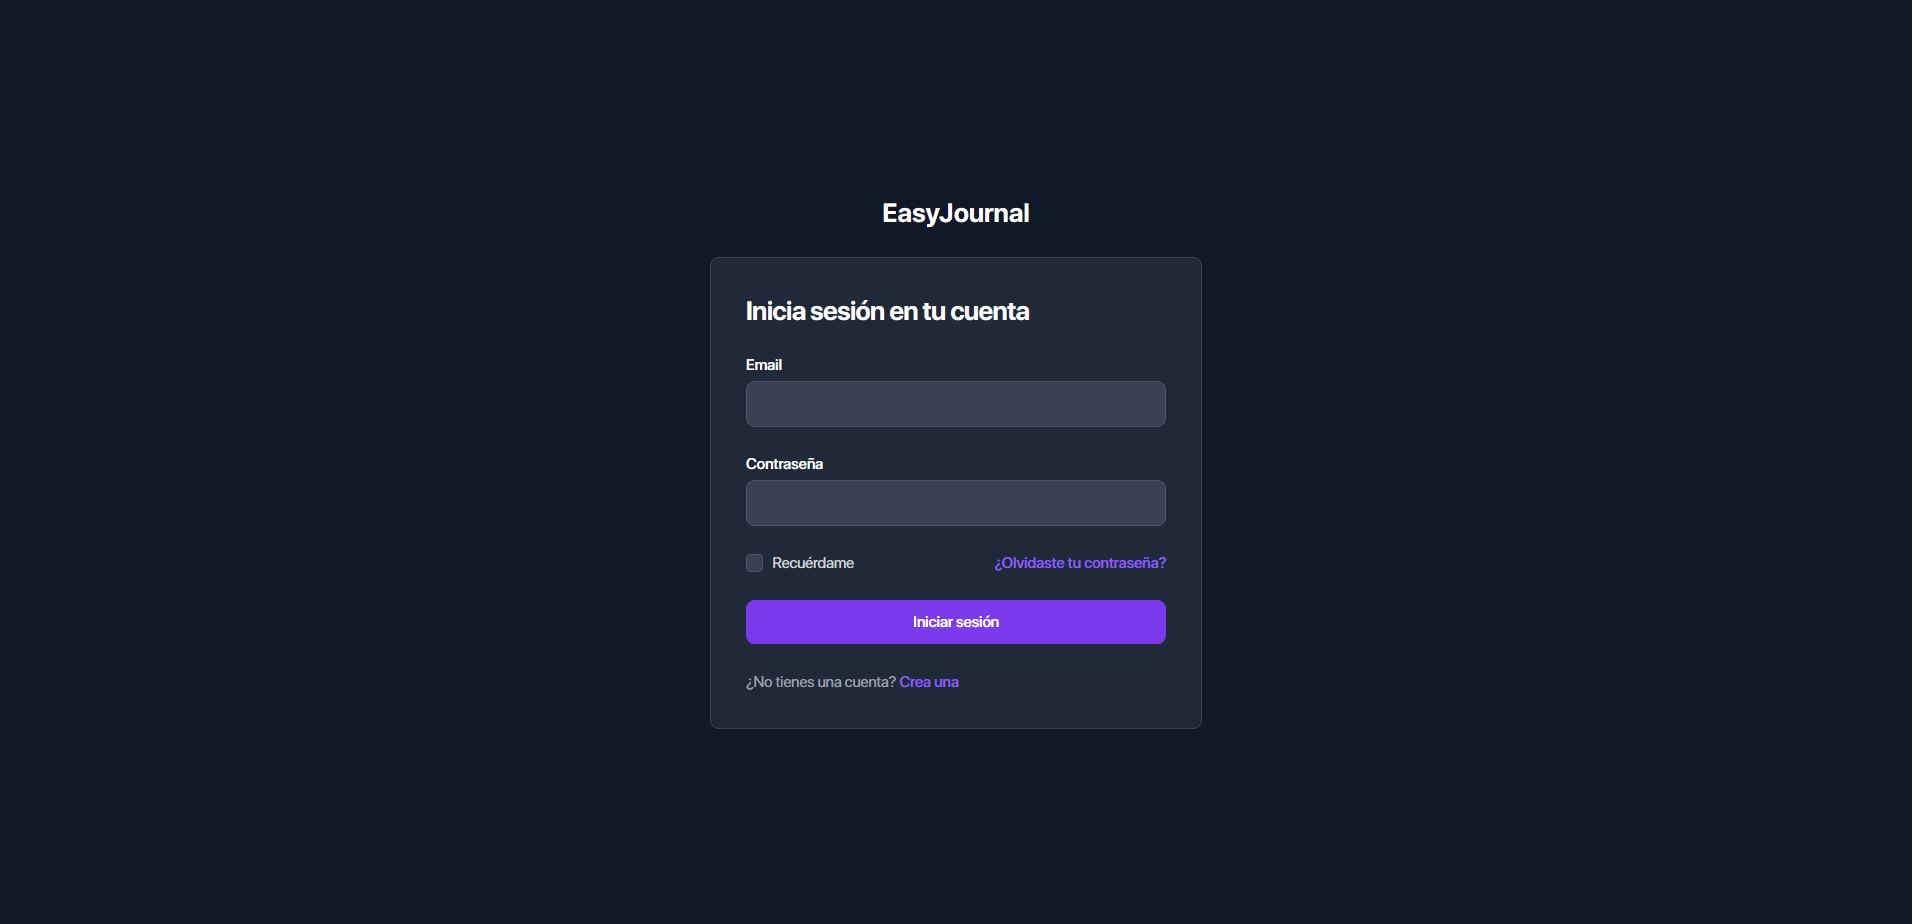
\includegraphics[width=1\textwidth]{IMAGENES/captura-1.png}
    \caption{Página de Inicio}
    \label{fig:captura-1}
\end{figure}

En la figura \ref{fig:captura-2} se muestra la página de creación de artículos, donde los usuarios pueden crear nuevos artículos, editar artículos existentes y ver una lista de todos los artículos creados.

\begin{figure}[H]
    \centering
    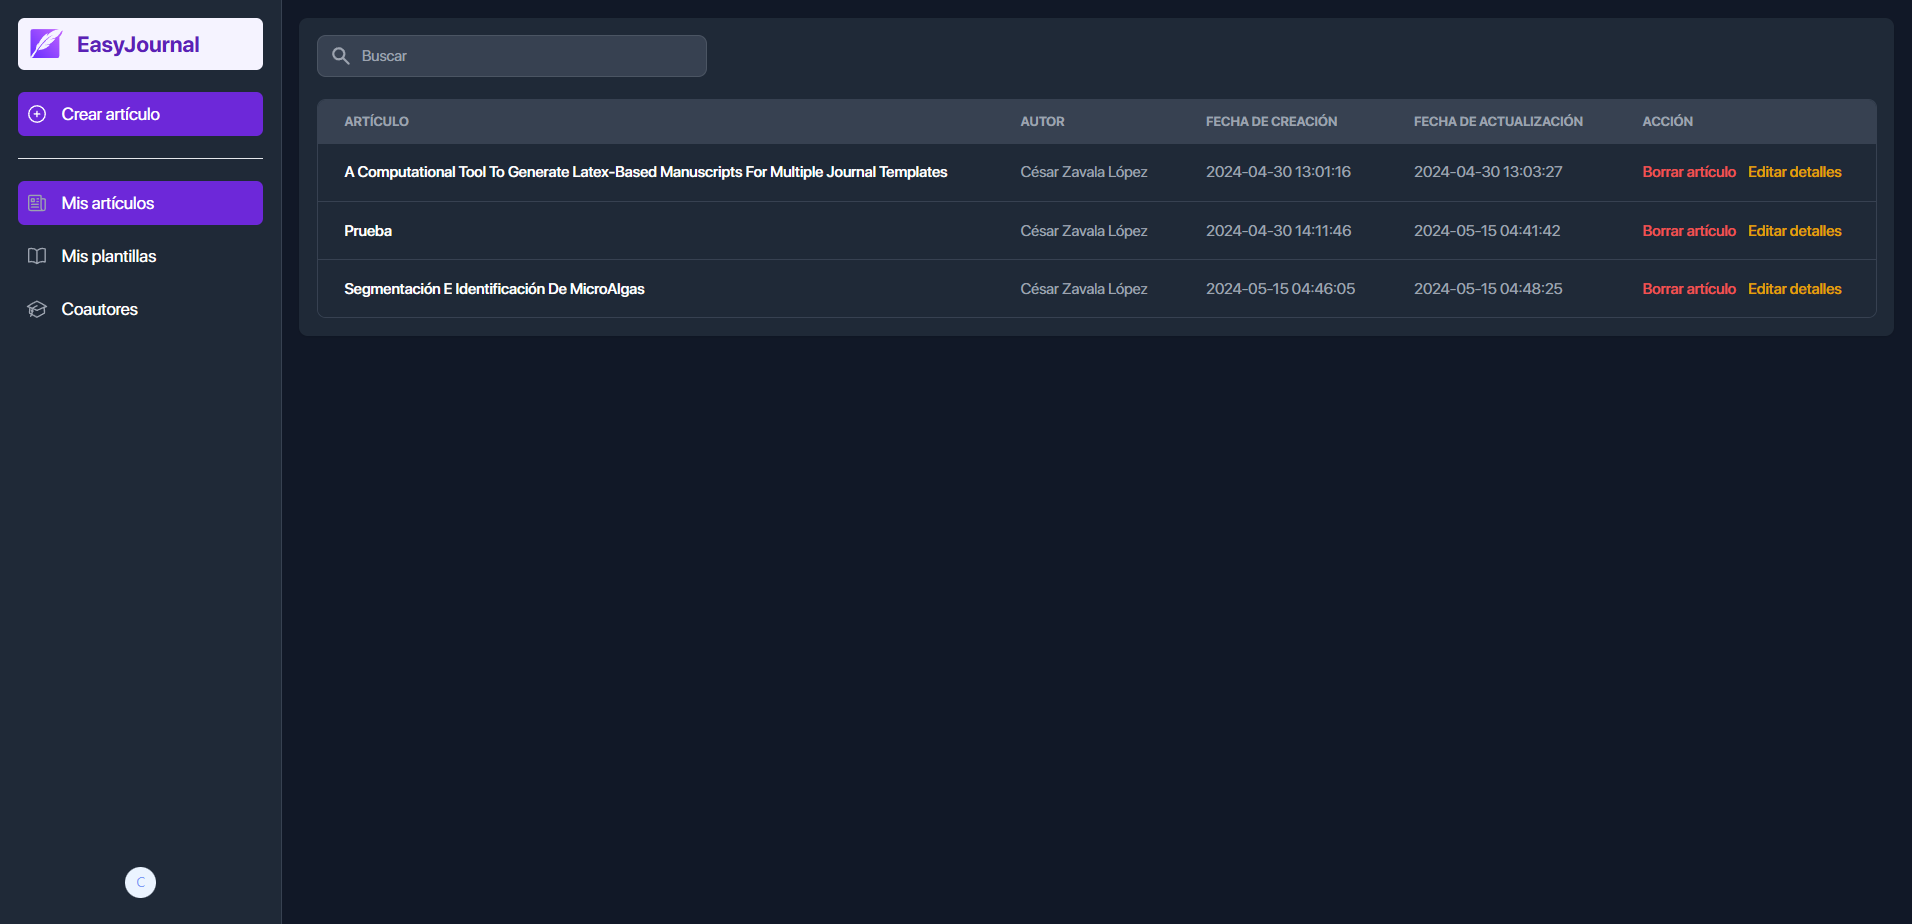
\includegraphics[width=1\textwidth]{IMAGENES/captura-2.png}
    \caption{Página de Creación de Artículos}
    \label{fig:captura-2}
\end{figure}

En la figura \ref{fig:captura-3} se muestra la página de gestión de coautores, donde los usuarios pueden agregar, editar y eliminar coautores a su lista de coautores.

\begin{figure}[H]
    \centering
    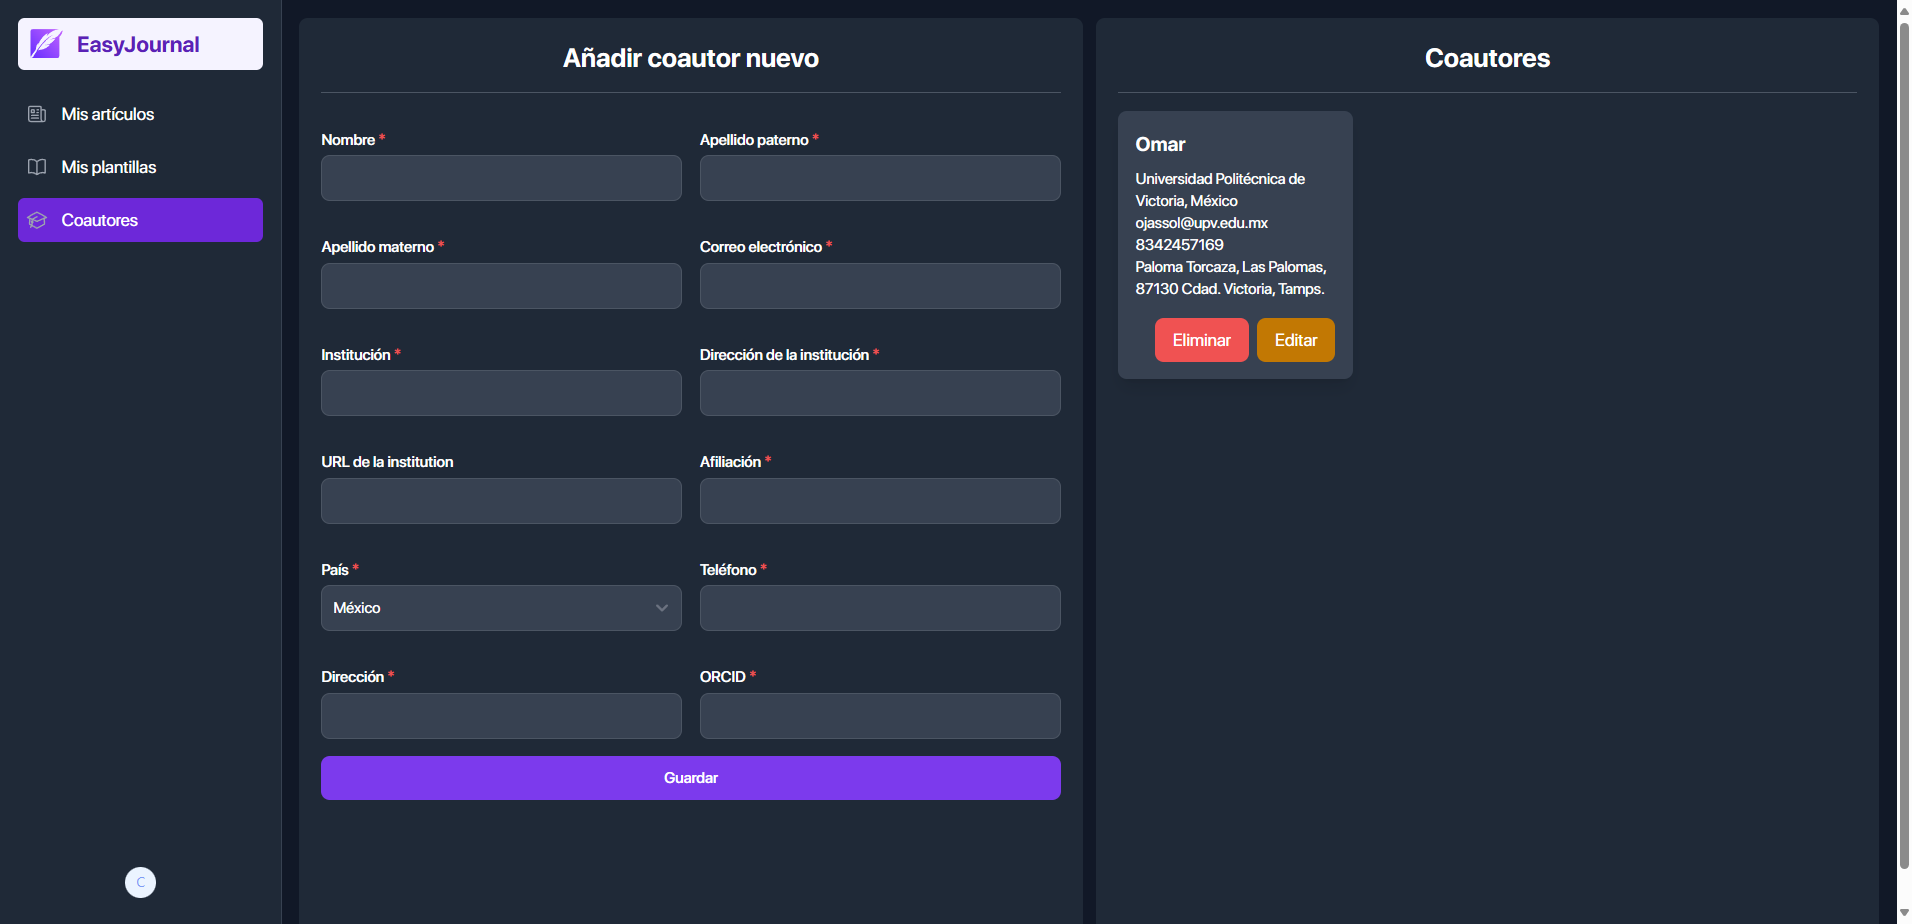
\includegraphics[width=1\textwidth]{IMAGENES/captura-3.png}
    \caption{Página de Gestión de Coautores}
    \label{fig:captura-3}
\end{figure}

En la figura \ref{fig:captura-4} se muestra la página de subida de plantillas LaTeX, donde los usuarios pueden subir plantillas LaTeX en formato .zip y previsualizarlas antes de compilarlas.

\begin{figure}[H]
    \centering
    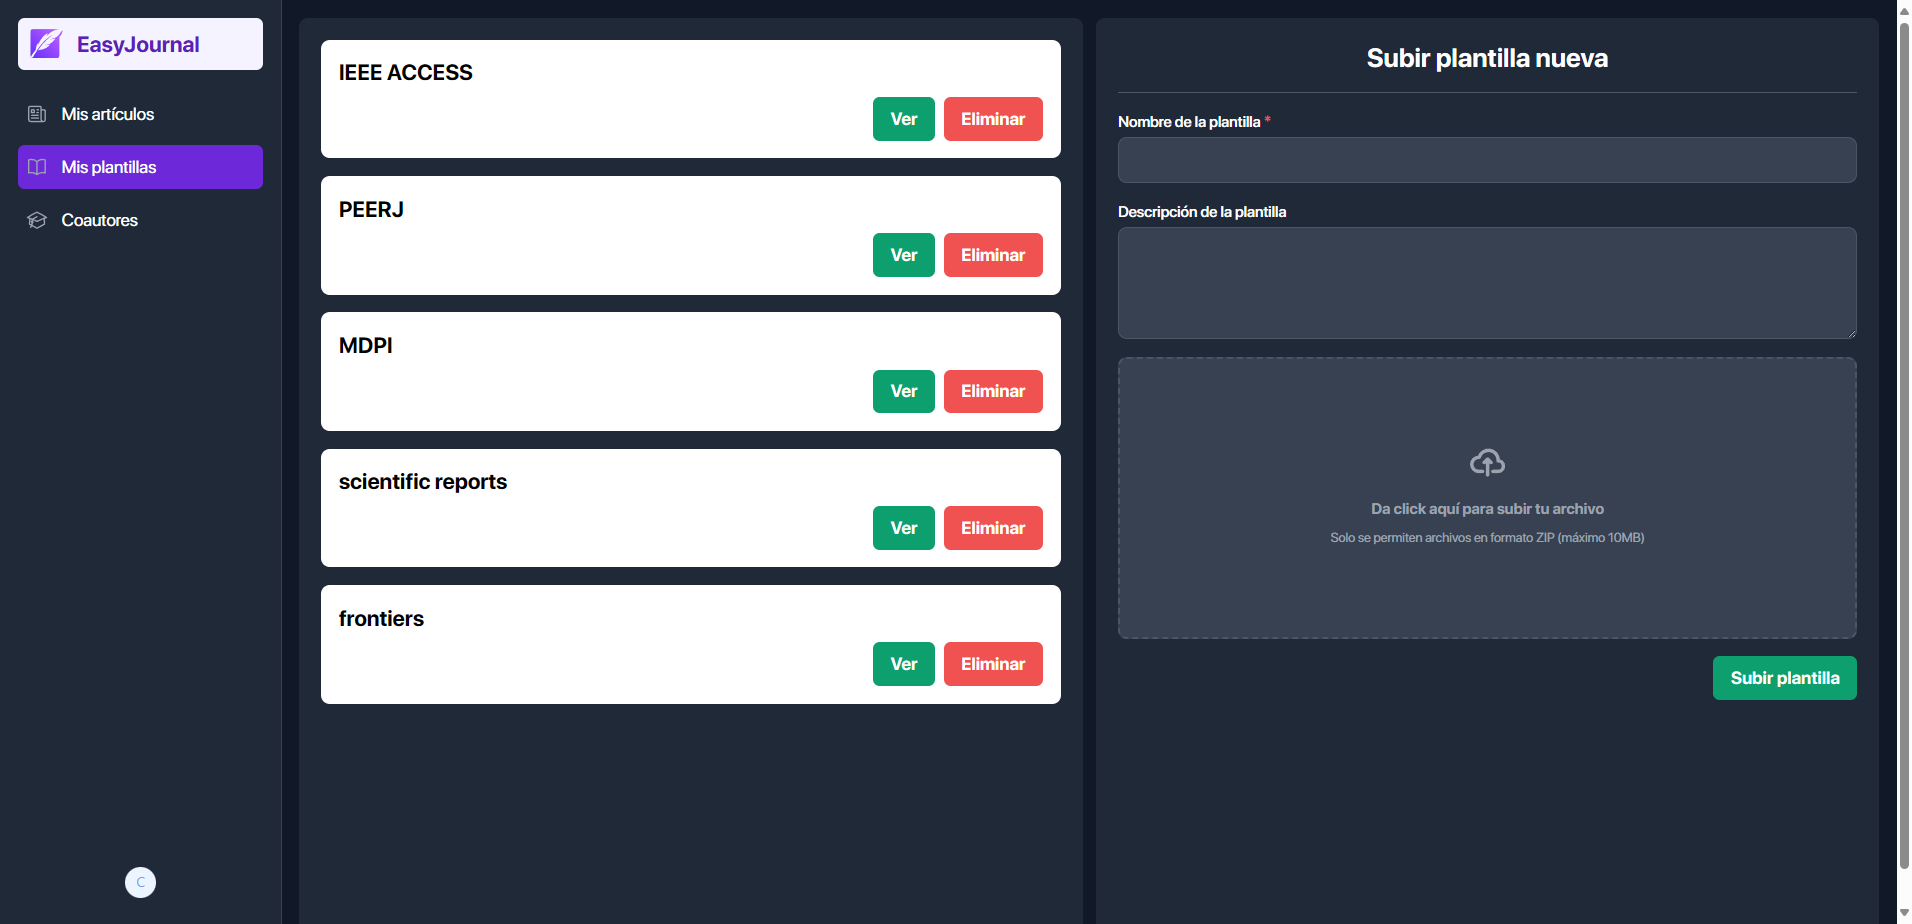
\includegraphics[width=1\textwidth]{IMAGENES/captura-4.png}
    \caption{Página de Subida de Plantillas LaTeX}
    \label{fig:captura-4}
\end{figure}

En la figura \ref{fig:captura-5} se muestra la página de previsualización de plantillas, donde los usuarios pueden ver una vista previa del archivo PDF generado a partir de la plantilla LaTeX.

\begin{figure}[H]
    \centering
    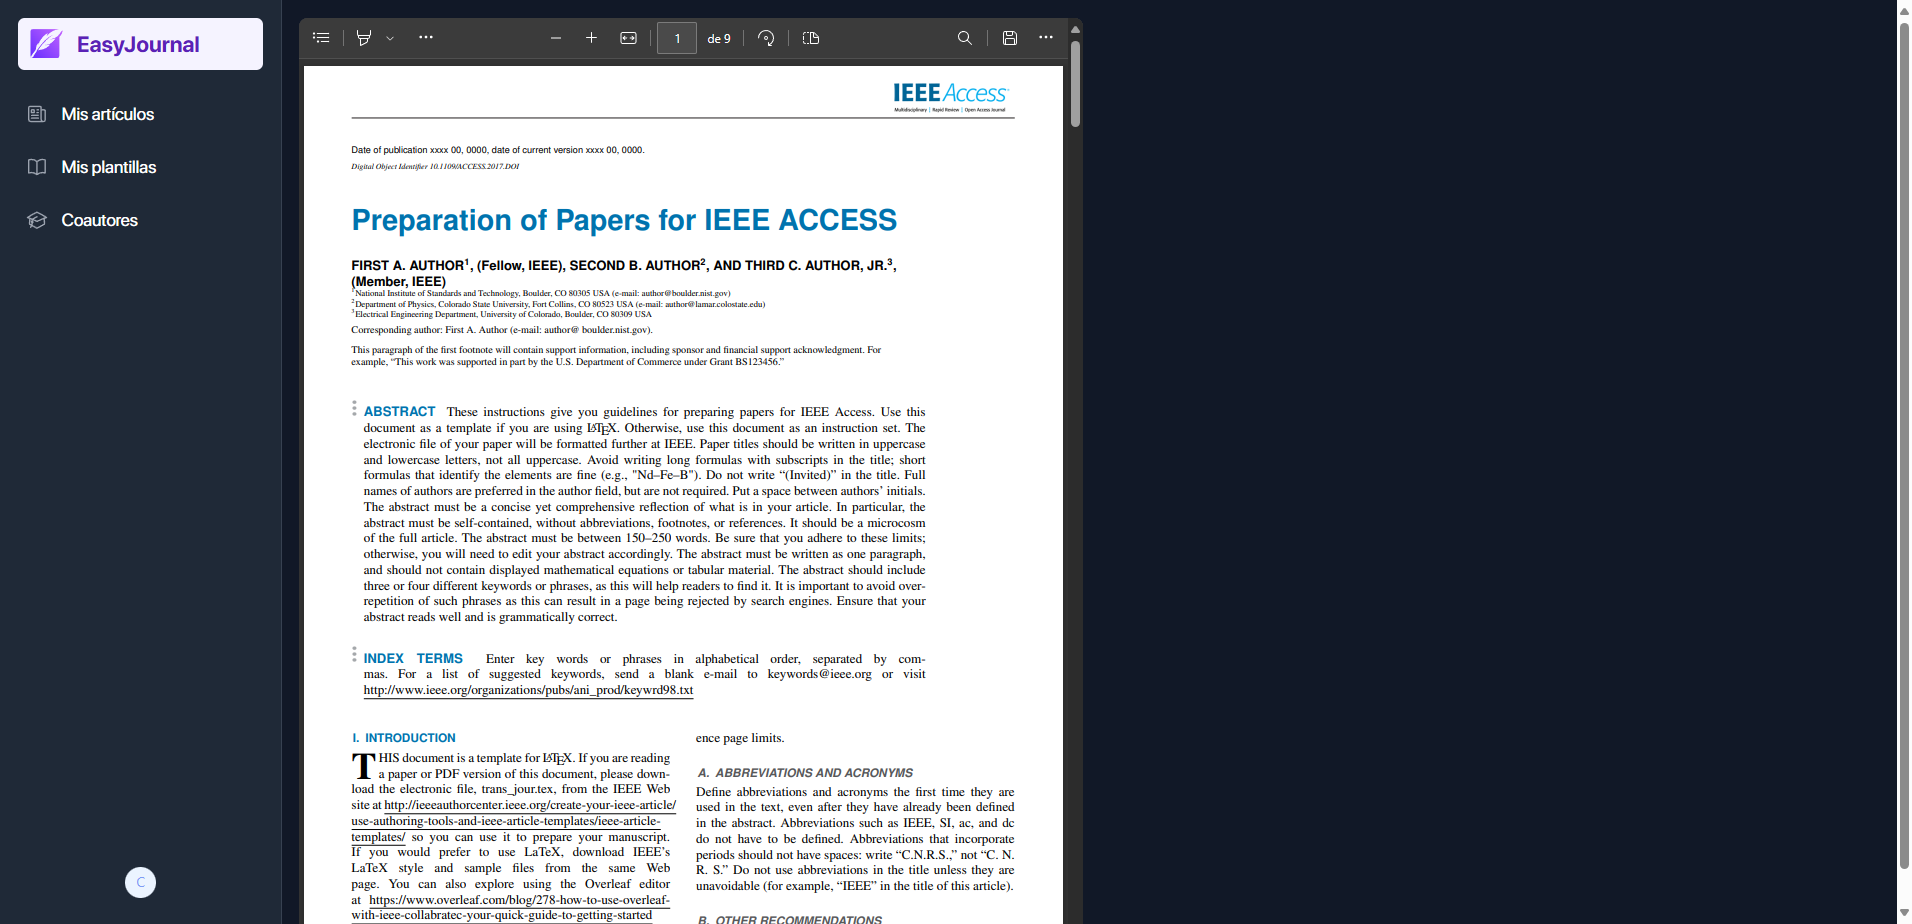
\includegraphics[width=1\textwidth]{IMAGENES/captura-5.png}
    \caption{Página de Previsualización de Plantillas}
    \label{fig:captura-5}
\end{figure}

En la figura \ref{fig:captura-6} se muestra la página de edición de perfil, donde los usuarios pueden editar su información personal, cambiar su contraseña y subir una foto de perfil.

\begin{figure}[H]
    \centering
    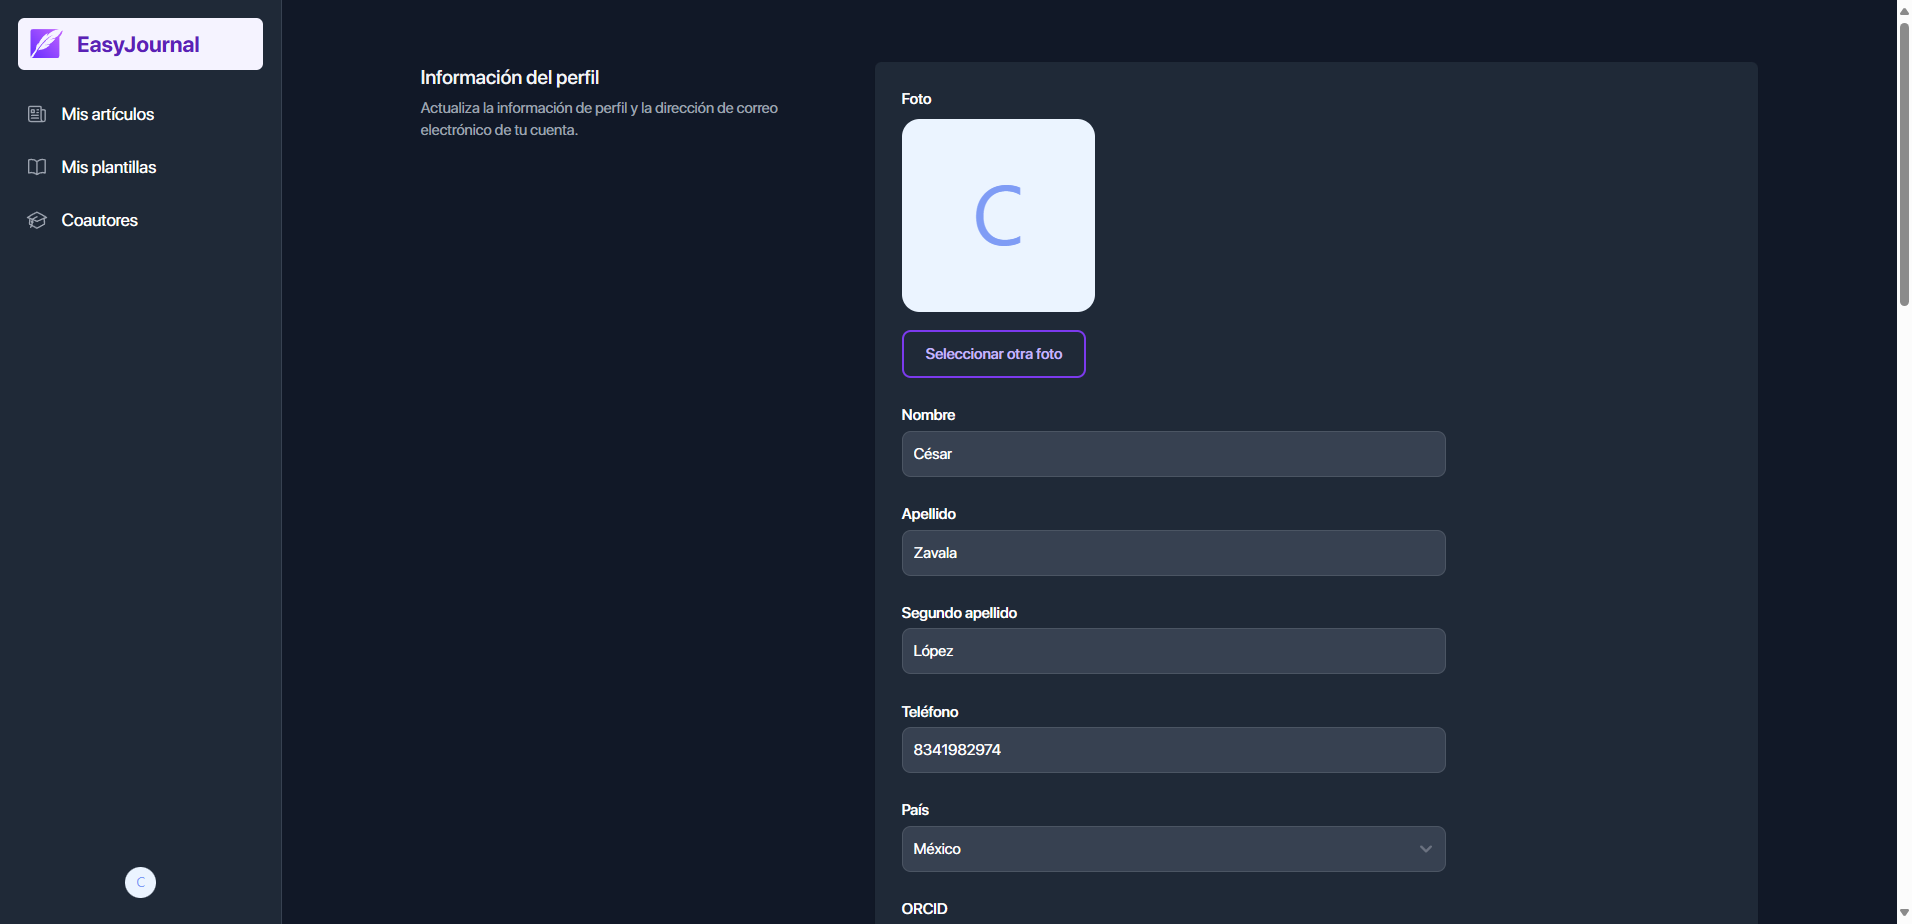
\includegraphics[width=1\textwidth]{IMAGENES/captura-6.png}
    \caption{Página de Edición de Perfil}
    \label{fig:captura-6}
\end{figure}

En la figura \ref{fig:captura-7} se muestra la página de recuperación de contraseña, donde los usuarios pueden restablecer su contraseña si la han olvidado.

\begin{figure}[H]
    \centering
    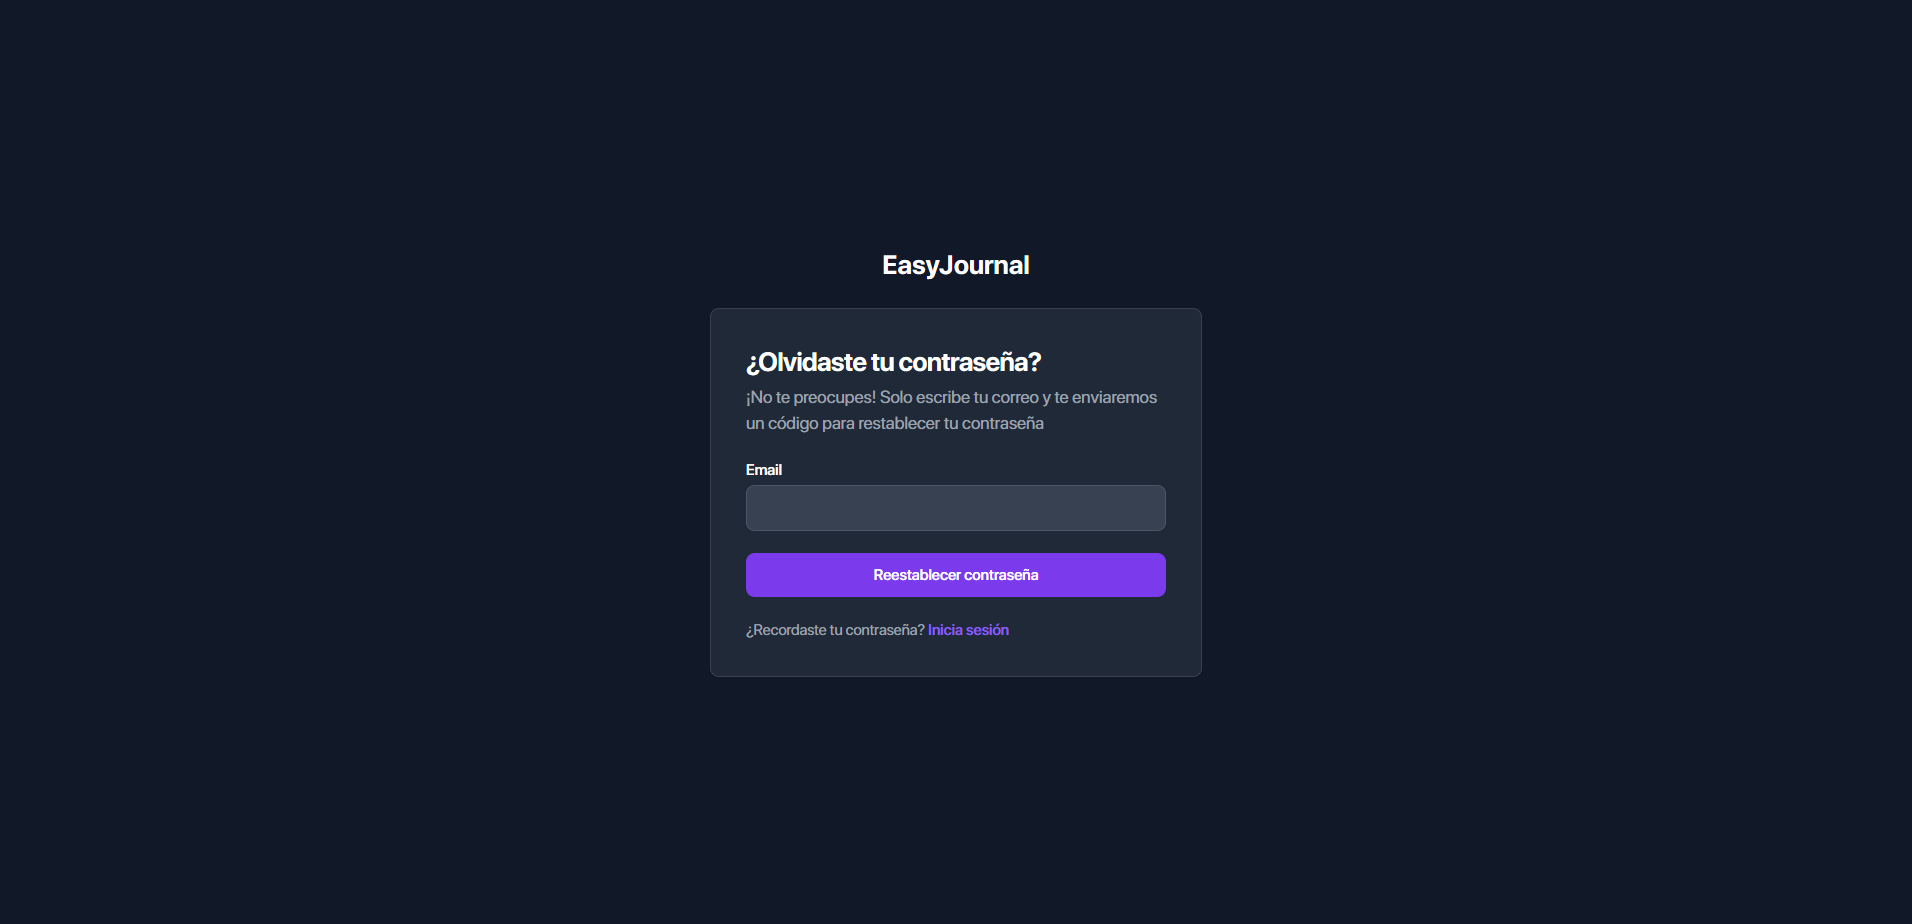
\includegraphics[width=1\textwidth]{IMAGENES/captura-7.png}
    \caption{Página de Recuperación de Contraseña}
    \label{fig:captura-7}
\end{figure}

En la figura \ref{fig:captura-8} se muestra la página de edición de artículo, donde los usuarios pueden editar un artículo existente, agregar contenido, imágenes y tablas, y compilar el artículo en una plantilla LaTeX.

\begin{figure}[H]
    \centering
    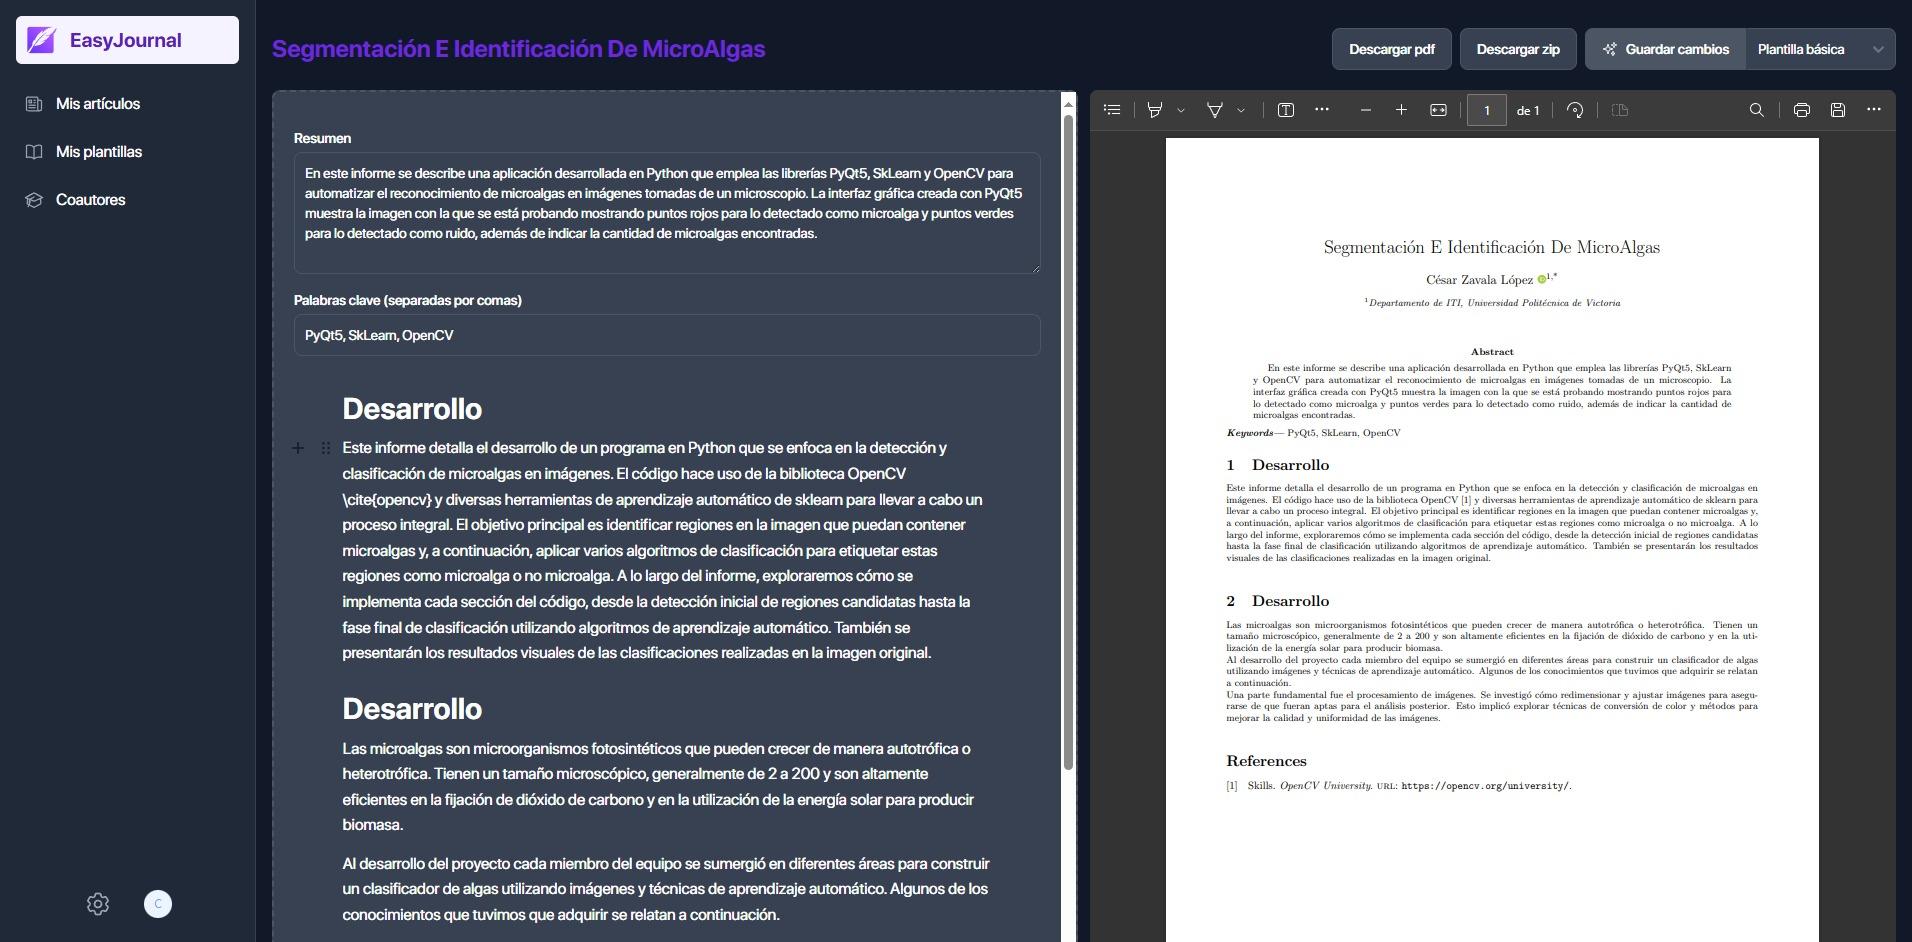
\includegraphics[width=1\textwidth]{IMAGENES/captura-8.png}
    \caption{Página de Edición de Artículo}
    \label{fig:captura-8}
\end{figure}

En la figura \ref{fig:captura-9} se muestra el resultado de la página de edición de artículo compilando la plantilla MDPI.

\begin{figure}[H]
    \centering
    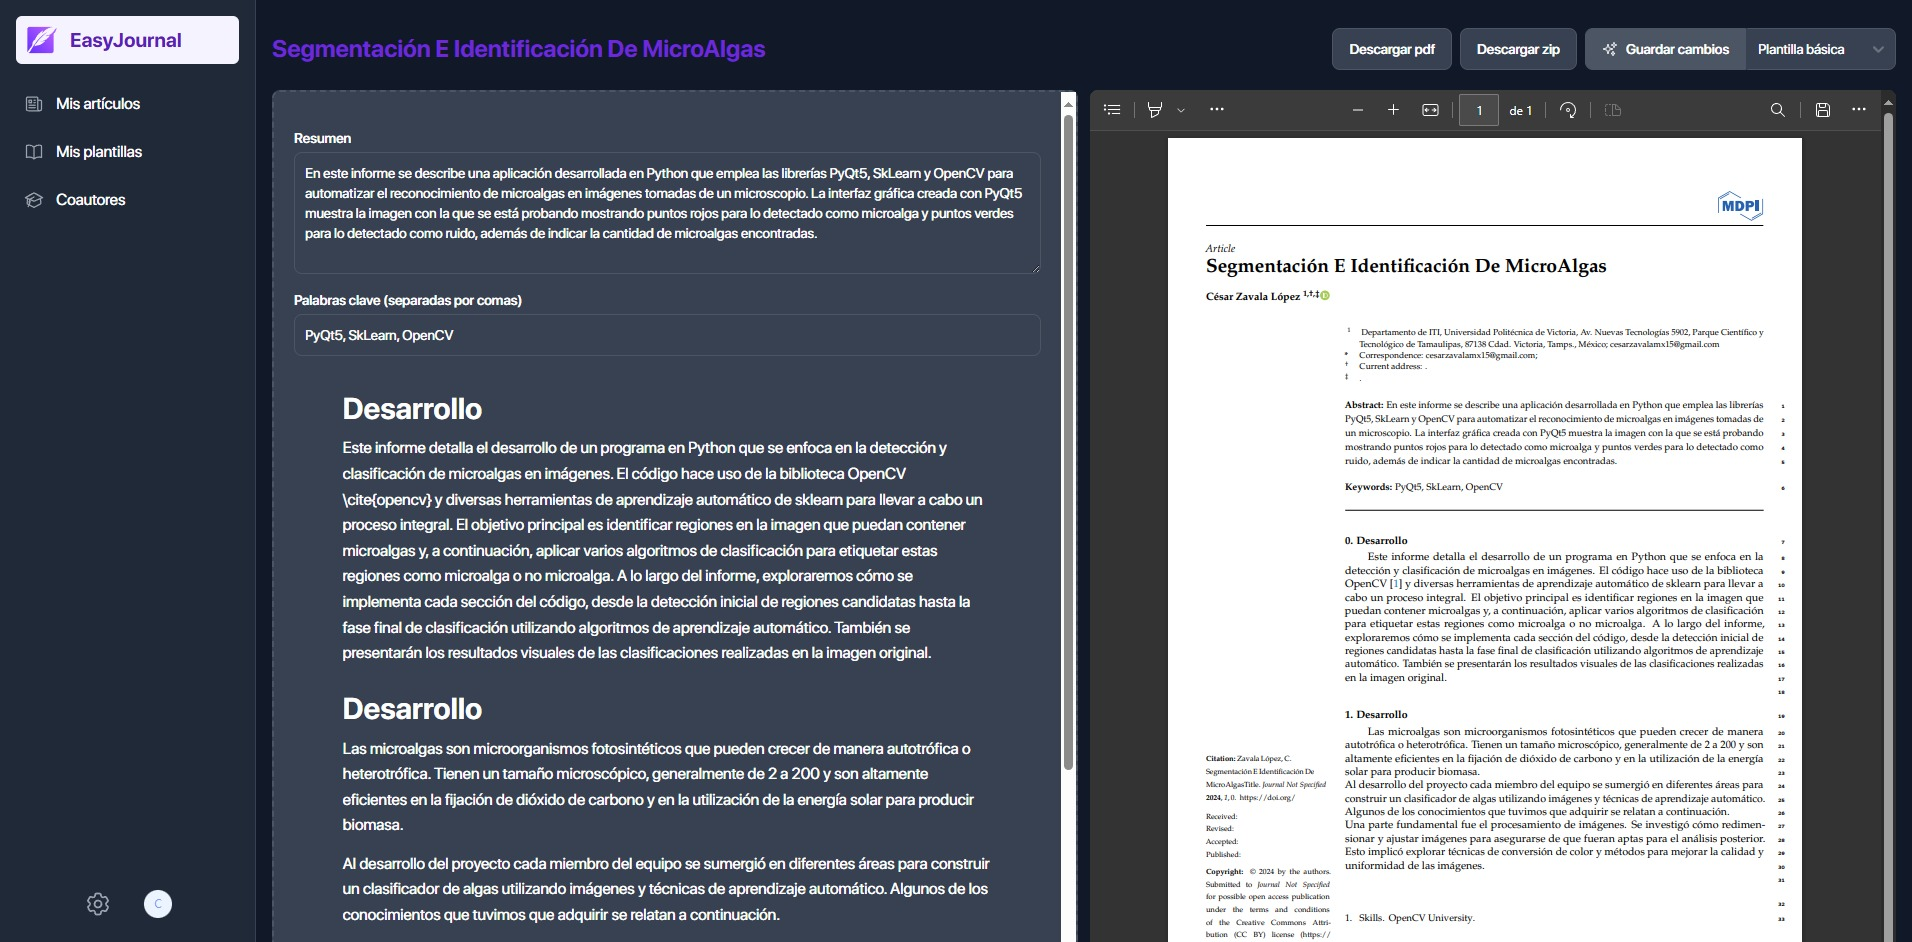
\includegraphics[width=1\textwidth]{IMAGENES/captura-9.png}
    \caption{Página de Edición de Artículo con plantilla MDPI}
    \label{fig:captura-9}
\end{figure}

En la figura \ref{fig:captura-10} se muestra el resultado de la página de edición de artículo compilando la plantilla frontiers.

\begin{figure}[H]
    \centering
    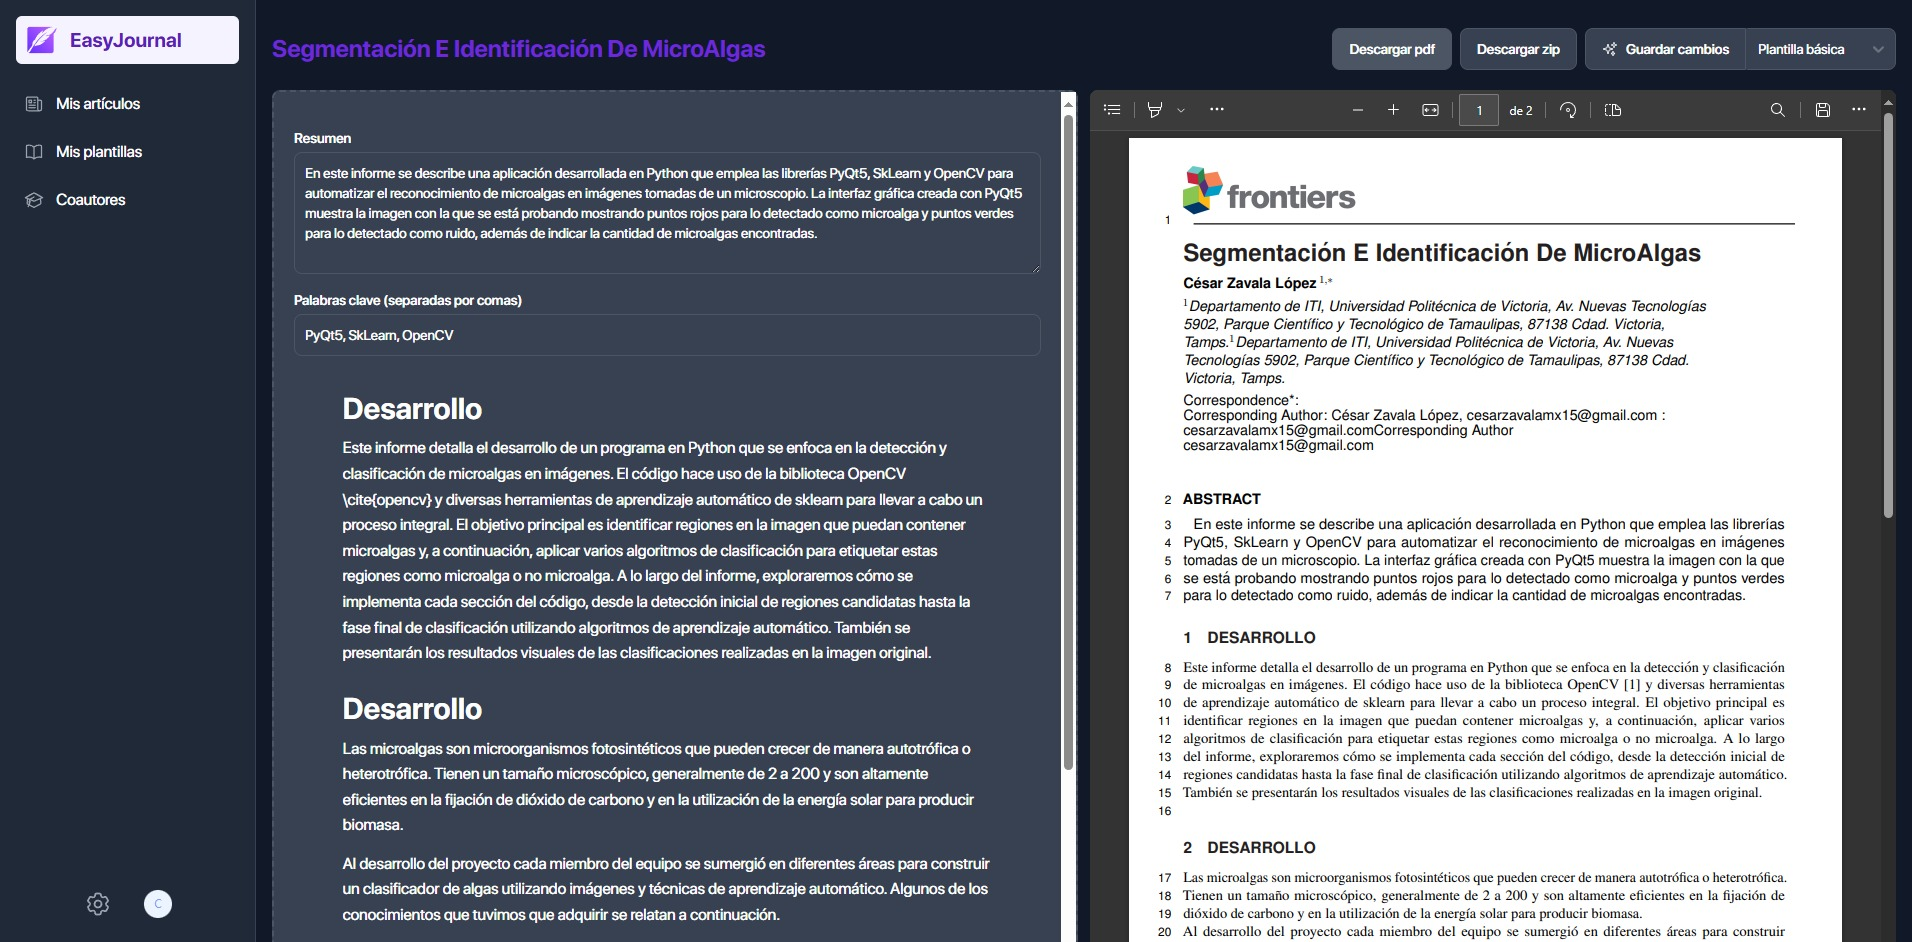
\includegraphics[width=1\textwidth]{IMAGENES/captura-10.png}
    \caption{Página de Edición de Artículo con plantilla frontiers}
    \label{fig:captura-10}
\end{figure}

En la figura \ref{fig:captura-11} se muestra el resultado de la página de edición de artículo compilando la plantilla Scientific Reports.

\begin{figure}[H]
    \centering
    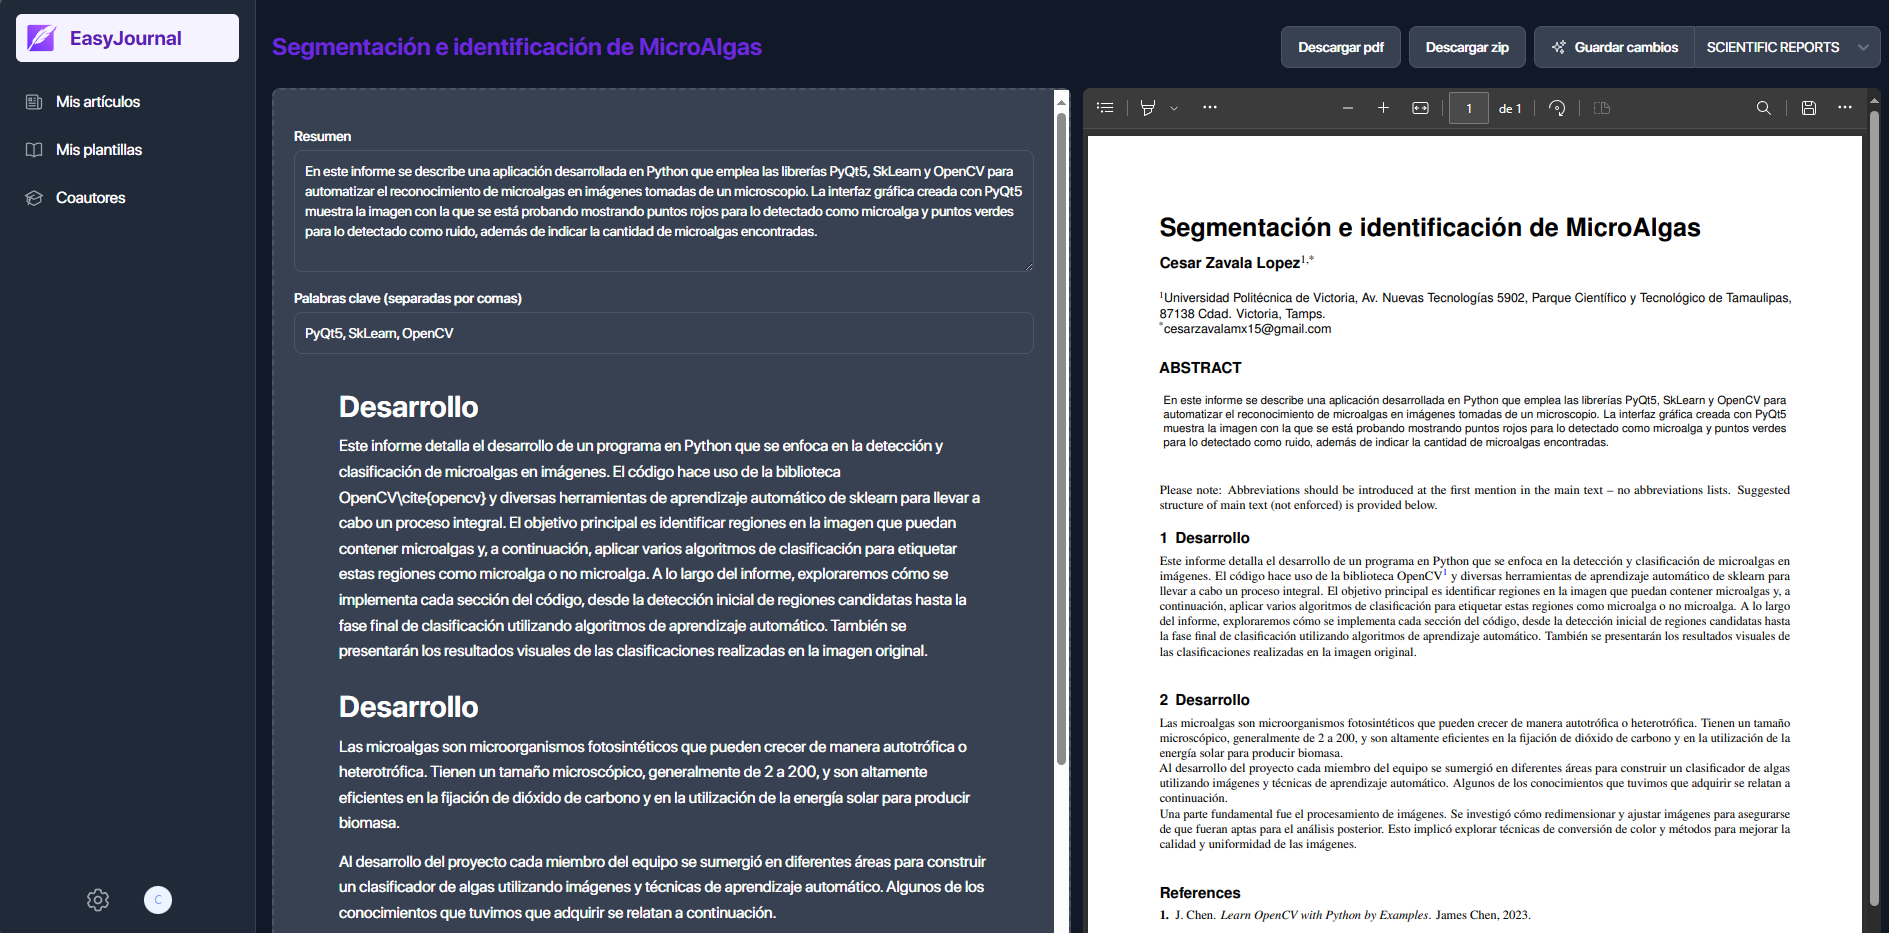
\includegraphics[width=1\textwidth]{IMAGENES/captura-11.png}
    \caption{Página de Edición de Artículo con plantilla Scientific Reports}
    \label{fig:captura-11}
\end{figure}

En la figura \ref{fig:captura-12} se muestra el resultado de la página de edición de artículo compilando la plantilla PeerJ.

\begin{figure}[H]
    \centering
    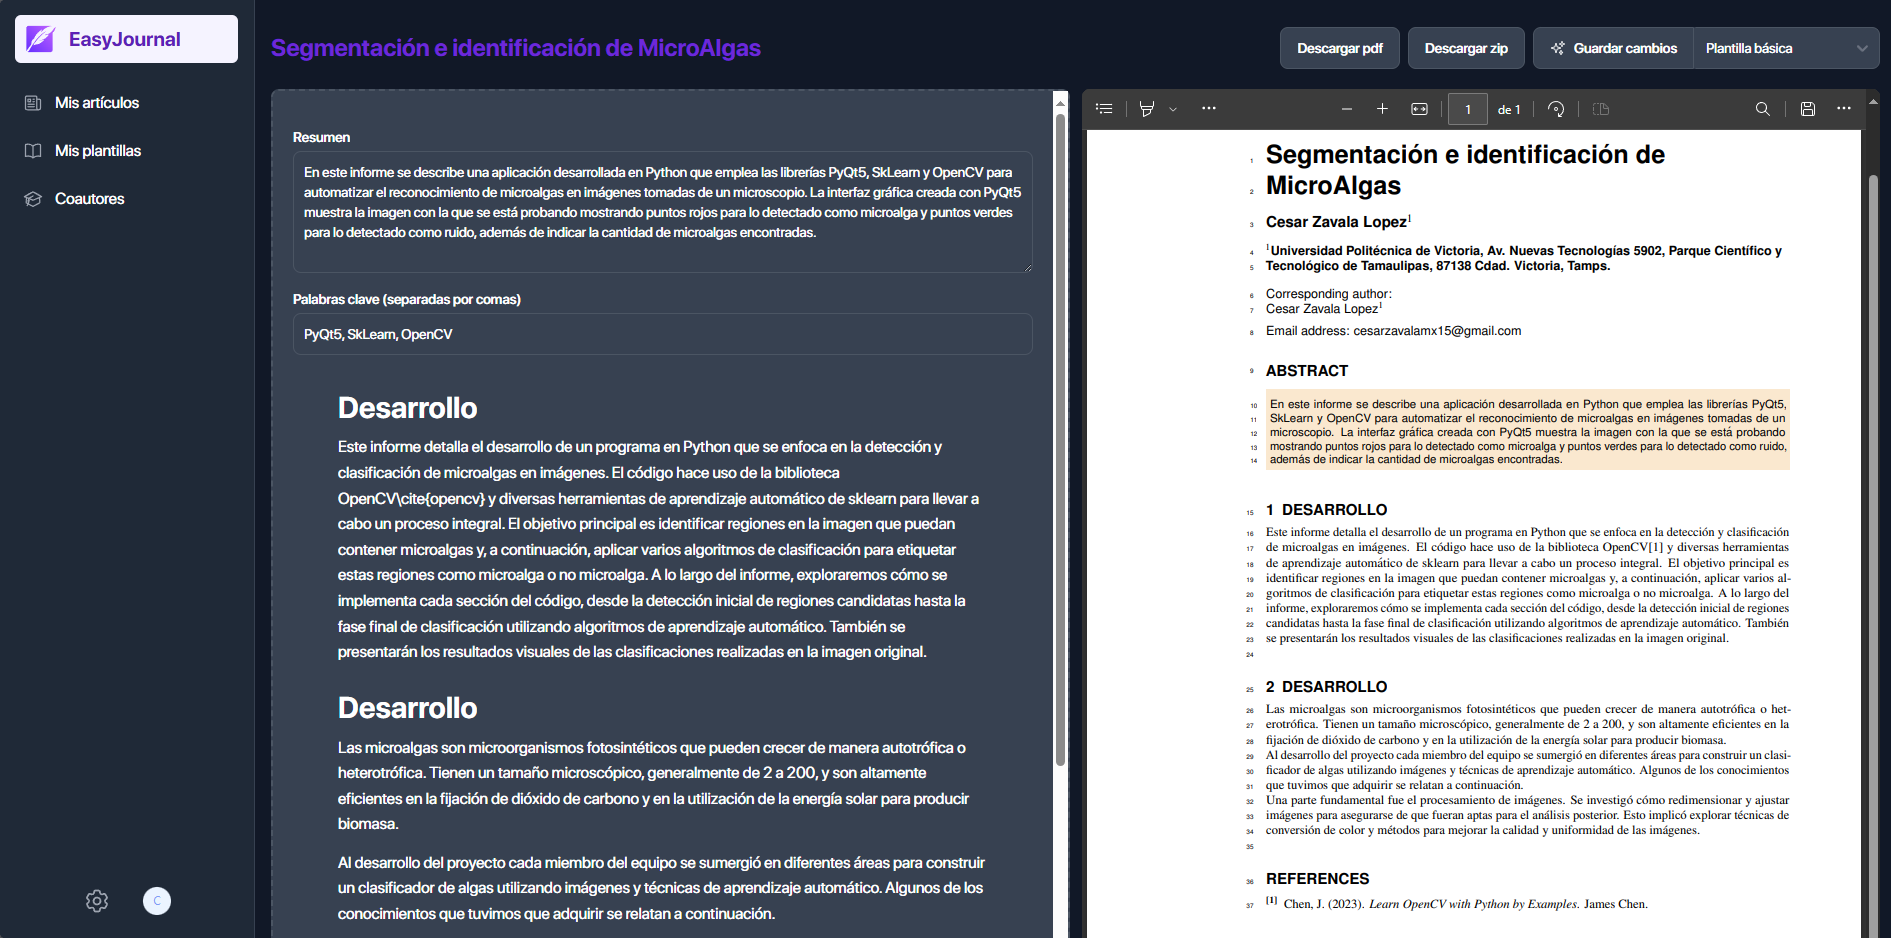
\includegraphics[width=1\textwidth]{IMAGENES/captura-12.png}
    \caption{Página de Edición de Artículo con plantilla PeerJ}
    \label{fig:captura-12}

\end{figure}

En la figura \ref{fig:captura-13} se muestra el resultado de la página de edición de artículo compilando la plantilla IEEE Access.

\begin{figure}[H]
    \centering
    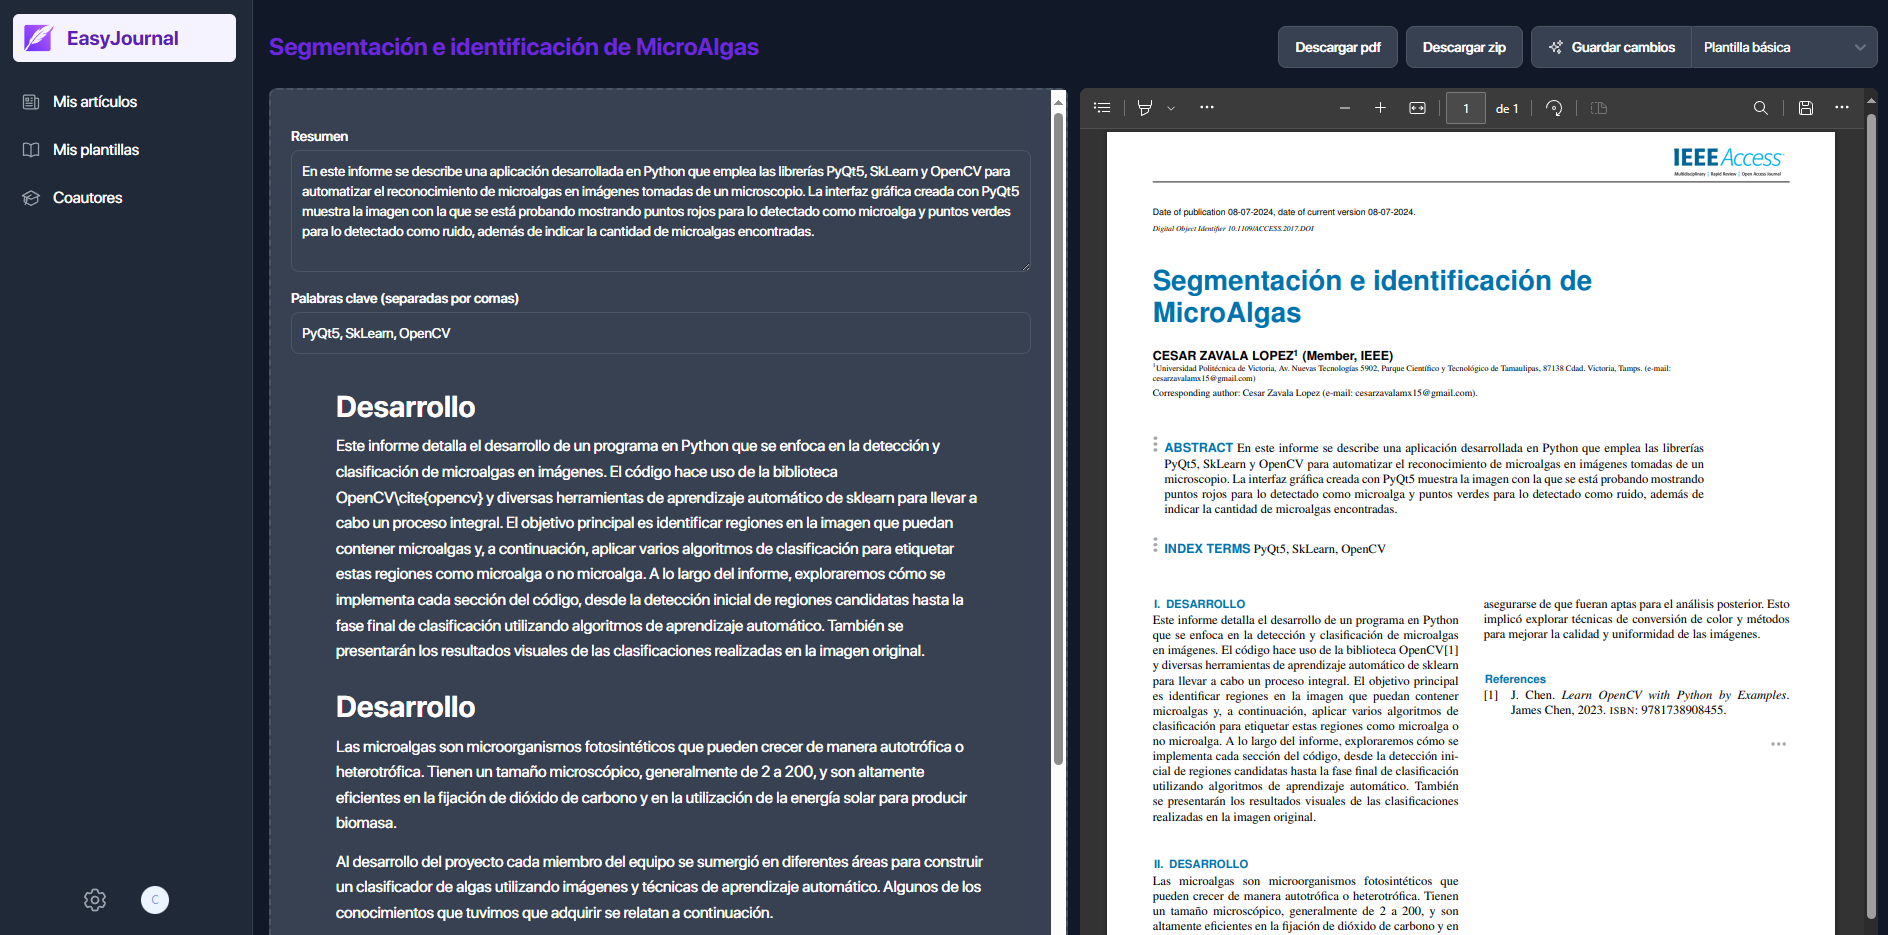
\includegraphics[width=1\textwidth]{IMAGENES/captura-13.png}
    \caption{Página de Edición de Artículo con plantilla IEEE Access}
    \label{fig:captura-13}
\end{figure}

\subsection{Análisis y Discusión de Resultados}
Los logros obtenidos durante el desarrollo del sistema son significativos y demuestran que el sistema cumple con los objetivos establecidos. Se implementaron todas las funcionalidades propuestas y se realizaron pruebas para garantizar el funcionamiento del sistema. Los resultados obtenidos muestran que todas las funcionalidades implementadas funcionan correctamente y que los usuarios pueden interactuar con el sistema de manera eficiente y sin problemas.

A continuación se presentan los logros principales del proyecto:

\begin{itemize}
    \item Se logró integrar Jetstream en el backend del sistema, lo que permitió establecer una base sólida de gestión de usuarios y facilitó el desarrollo de la aplicación.
    \item Se implementó un sistema de gestión de plantillas LaTeX que permite a los usuarios subir plantillas en formato .zip, previsualizarlas y compilarlas en archivos PDF.
    \item Se implementó un sistema de gestión de artículos que permite a los usuarios crear, editar y compilar artículos en plantillas LaTeX.
    \item Se implementó un sistema de gestión de coautores que permite a los usuarios agregar, editar y eliminar coautores de un artículo.
    \item Se implementó un sistema de gestión de archivos que protege los archivos de acceso no autorizado y garantiza la seguridad de los datos.
    \item Se implementó un sistema de validación de plantillas que verifica la estructura y los archivos de la plantilla antes de compilarla.
    \item Se implementó un sistema de seguridad que protege el sistema contra ataques de inyección SQL, XSS, CSRF, fuerza bruta y exposición de datos sensibles.
\end{itemize}   

El impacto del sistema se espera que sea significativo, ya que proporciona una solución innovadora y eficiente para la creación y edición de artículos científicos en formato LaTeX. La implementación de esta herramienta permite a los usuarios generar documentos de alta calidad de manera rápida y sencilla, lo que facilita la colaboración y la comunicación en el ámbito académico y científico. 



\clearpage
\section{Conclusiones y Trabajos Futuros}
Para finalizar con este documento es necesario abordar con las conclusiones obtenidas a lo largo de este proceso de desarrollo, también es importante tener en cuenta el trabajo a futuro y proponer mejoras en todo lo que no pudo realizarse, teniendo en cuenta siempre un progreso notable en el proyecto. 

\subsection{Conclusiones del Proyecto}
Este proyecto tuvo como objetivo principal desarrollar un sistema de formateo de artículos científicos en formato LaTeX, que permita al usuario subir plantillas LaTeX, crear y editar artículos, y compilarlos en archivos PDF. Esto con el objetivo de facilitar la creación y edición de artículos en la comunidad científica y académica, debido a que existen diferentes plantillas LaTeX para diferentes revistas y conferencias, lo que dificulta el proceso de formateo de los artículos, siendo poco eficiente tener que cambiar manualmente el formato de los artículos para cumplir con los requisitos de las plantillas.

Durante el desarrollo del proyecto, se llevaron a cabo diversas actividades de investigación, diseño, desarrollo, implementación y pruebas para garantizar el funcionamiento del sistema. Se establecieron procesos y procedimientos detallados para cada etapa del proyecto para minimizar los problemas y garantizar la calidad del sistema. 

Uno de los principales desafíos durante el desarrollo fue la integración de diversas tecnologías y que funcionaran de manera conjunta. La combinación tecnologías permitió crear una plataforma robusta y versátil para la creación y edición de documentos. Sin embargo, se encontraron dificultades en la configuración inicial del entorno de desarrollo y en la integración de algunas herramientas, lo que requirió un esfuerzo adicional para resolver.

A pesar de los desafíos, el proyecto logró cumplir con los objetivos establecidos y proporcionar una solución funcional para la edición de artículos en formato LaTeX.

\subsection{Trabajos Futuros}
Aunque el proyecto ha alcanzado sus objetivos principales, aún existen áreas que pueden mejorarse y funcionalidades adicionales que pueden agregarse en el futuro. Algunas de las posibles mejoras y trabajos futuros incluyen:

\begin{itemize}
\item Implementación de autenticación con Google para permitir el inicio de sesión y el registro mediante cuentas de Google, lo que mejoraría la experiencia del usuario y aumentaría la seguridad del sistema.
\item Incorporación de funciones avanzadas de LaTeX, como soporte para ecuaciones matemáticas complejas, referencias cruzadas y bibliografía automática, para proporcionar a los usuarios herramientas más avanzadas para la creación de artículos científicos.
\item Desarrollo de una función de navegación por bloques en el editor de artículos, que permita a los usuarios moverse fácilmente entre diferentes secciones y elementos del documento, facilitando la organización y edición del contenido.
\item Optimización del tiempo de compilación de los documentos LaTeX, mediante la implementación de técnicas de paralelización o la optimización de los procesos de compilación, para reducir el tiempo necesario para generar los archivos PDF.
\end{itemize}

Estas mejoras y trabajos futuros pueden contribuir a mejorar la funcionalidad, usabilidad y rendimiento del sistema, permitiendo así satisfacer mejor las necesidades de los usuarios y proporcionar una experiencia más fluida. El proyecto tiene un gran potencial para seguir creciendo y evolucionando en el futuro, se espera que el desarrollo realizado hasta el momento sea un punto de partida para futuras mejoras y actualizaciones.





\clearpage
% \pagenumbering{roman}
% \setcounter{page}{6}
\addcontentsline{toc}{section}{Índice de figuras}
\renewcommand\listfigurename{Índice de figuras}

\listoffigures

\clearpage
\addcontentsline{toc}{section}{Índice de cuadros}
\renewcommand\listtablename{Índice de cuadros}
\listoftables

\clearpage
\addcontentsline{toc}{section}{Índice de algoritmos}
\renewcommand\listalgorithmname{Índice de algoritmos}
\listofalgorithms{}

%-----------------------------------------------------------------------------------------------------------------
% REFERENCIAS


\clearpage
%Let's cite! The Einstein's journal paper \cite{dirac} and the Dirac's 
%book \cite{einstein} are physics related items. 

%\Urlmuskip=0mu plus 1mu\relax
\addcontentsline{toc}{section}{Referencias} 
\printbibliography{}
 
\end{document}
